% Some classes load the `subfigure` package which clashes with
% our internal use of `subfig` for subfloats. We are most likely
% not going to need the canned subfigure functionality anyways,
% so we'll trick LaTeX into thinking it already loaded `subfigure`
\makeatletter
\newcommand{\dontusepackage}[2][]{%
  \@namedef{ver@#2.sty}{9999/12/31}%
  \@namedef{opt@#2.sty}{#1}}
\makeatother
\dontusepackage{subfigure}


%% ===== Begin LaTeX file ===========================
%%
\documentclass[12pt,a4paper,]{report}

\usepackage{lmodern}
\usepackage{setspace}
\setstretch{1.5}
\usepackage{amssymb,amsmath}
\usepackage{ifxetex,ifluatex}
\usepackage[usenames,dvipsnames]{color}
\usepackage{fixltx2e} % provides \textsubscript
\ifnum 0\ifxetex 1\fi\ifluatex 1\fi=0 % if pdftex
  \usepackage[T1]{fontenc}
  \usepackage[utf8]{inputenc}
\else % if luatex or xelatex
  \ifxetex
    \usepackage{mathspec}
    \usepackage{xltxtra,xunicode}
  \else
    \usepackage{fontspec}
  \fi
  \defaultfontfeatures{Mapping=tex-text,Scale=MatchLowercase}
  \newcommand{\euro}{€}
    \setmainfont{Arial}
\fi
% use upquote if available, for straight quotes in verbatim environments
\IfFileExists{upquote.sty}{\usepackage{upquote}}{}
% use microtype if available
\IfFileExists{microtype.sty}{%
\usepackage{microtype}
\UseMicrotypeSet[protrusion]{basicmath} % disable protrusion for tt fonts
}{}
\usepackage[vmargin=2.5cm,hmargin=2.5cm]{geometry}
\usepackage{listings}
% Define slightly more reasonable Listings defaults
\lstset{
    basicstyle=\ttfamily\small,
    breaklines=true,
    prebreak=\raisebox{0ex}[0ex][0ex]{\ensuremath{\hookleftarrow}},
    frame=lines,
    showtabs=false,
    showspaces=false,
    showstringspaces=false,
    keywordstyle=\color[gray]{0.4}\bfseries,
    commentstyle=\color[gray]{0.65}\itshape,
    numbers=left,
    captionpos=b,
}
\usepackage{longtable,booktabs}
\usepackage{graphicx}
\makeatletter
\def\maxwidth{\ifdim\Gin@nat@width>\linewidth\linewidth\else\Gin@nat@width\fi}
\def\maxheight{\ifdim\Gin@nat@height>\textheight\textheight\else\Gin@nat@height\fi}
\makeatother
% Scale images if necessary, so that they will not overflow the page
% margins by default, and it is still possible to overwrite the defaults
% using explicit options in \includegraphics[width, height, ...]{}
\setkeys{Gin}{width=\maxwidth,height=\maxheight,keepaspectratio}
\usepackage{caption}
\usepackage{float}
% Override extremely conservative LaTeX float placement rules
% (might need to be removed for "manuscript" styles)
\renewcommand{\topfraction}{0.85}	% max fraction of floats at top
\renewcommand{\bottomfraction}{0.75}	% max fraction of floats at bottom
\setcounter{topnumber}{2}
\setcounter{bottomnumber}{2}
\setcounter{totalnumber}{4}
\setcounter{dbltopnumber}{2}    % for 2-column pages
\renewcommand{\dbltopfraction}{0.85}	% fit big float above 2-col. text
\renewcommand{\textfraction}{0.10}	% allow minimal text w. figs
\renewcommand{\floatpagefraction}{0.85}	% require fuller float pages
\renewcommand{\dblfloatpagefraction}{0.85}	% require fuller float pages
% Encourage floats to be placed in the vacinity of where it is defined
% (in some manuscript styles where figures are collected at the end, the 'h'
% option might need to be removed by a separate '\floatplacement' call in the
% 'header-includes' metadata field)
\floatplacement{figure}{htbp}
\floatplacement{scholmdAlgorithm}{htbp}
\floatplacement{table}{htbp}
\usepackage{subfig}
\captionsetup[subfloat]{margin=1em}
\ifxetex
  \usepackage[setpagesize=false, % page size defined by xetex
              unicode=false, % unicode breaks when used with xetex
              xetex]{hyperref}
\else
  \usepackage[unicode=true]{hyperref}
\fi
\hypersetup{breaklinks=true,
            bookmarks=true,
            pdfauthor={},
            pdftitle={},
            colorlinks=true,
            citecolor=black,
            urlcolor=blue,
            linkcolor=black,
            pdfborder={0 0 0}}
\urlstyle{same}  % don't use monospace font for urls
\setlength{\parindent}{0pt}
\setlength{\parskip}{6pt plus 2pt minus 1pt}
\setlength{\emergencystretch}{3em}  % prevent overfull lines
\setcounter{secnumdepth}{5}


\date{}

% \usepackage[onehalfspacing]{setspace}

\usepackage{titlesec}
% Set number format of titles
\titleformat{\chapter}[hang]{\bfseries\huge}{\thechapter.}{2pc}{}
\titlelabel{\thetitle.\:}
% Decrease spacing above and below chapter titles
\titlespacing*{\chapter}{0pt}{-10pt}{30pt}

% Number figures for whole document and not chapter-wise
\usepackage{chngcntr}
\counterwithout{figure}{chapter}
\counterwithout{table}{chapter}
\counterwithout{equation}{chapter}

% Change identifier in figure caption
%\renewcommand{\figurename}{Fig.}

% Center figure captions and make Figure bold
\usepackage[labelfont=bf,justification=centering]{caption}

% Put captions above tables
\usepackage{float}
\floatstyle{plaintop}
\restylefloat{table}

%\usepackage{wrapfig}

% Increase spacing above and below figures/tables
\setlength{\intextsep}{12mm}

% Change names for lists
\renewcommand{\listfigurename}{Figures}
\renewcommand{\listtablename}{Tables}

% Center figures
% \makeatletter
% \g@addto@macro\@floatboxreset\centering
% \makeatother


% \usepackage{titling}
% \pretitle{\LARGE\bfseries}
% \posttitle{\par\vskip 0.5em \ Bachelor Thesis in Physics \ by}
% \preauthor{\begin{center}
% \large \lineskip 0.5em%
% \begin{tabular}[t]{c}}
% \postauthor{\end{tabular}\par\end{center}}
% \predate{\begin{center}\large}
% \postdate{\par\end{center}}


\begin{document}

\begin{titlepage}

\centering\large
\vspace*{1.5cm}

{\LARGE\bf Characterizing the dynamics of a \textit{Drosophila} motoneuron model via bifurcation analysis}

\vspace{1.5cm}

\textbf{Bachelor Thesis in Physics}

by

\textbf{Johannes Rieke}

12 January 2016

\vspace{1.5cm}

Friedrich-Alexander-Universität Erlangen-Nürnberg

\vspace{1.5cm}

\includegraphics[width=0.3\textwidth]{images/fau-siegel.pdf}\par
\vspace{1.5cm}

Supervisor: Prof. Klaus Mecke

\end{titlepage}

\chapter*{Abstract}\label{abstract}
\addcontentsline{toc}{chapter}{Abstract}

A recently published computational model of the motoneuron MN1-Ib (aCC)
in the third instar larva of \emph{Drosophila} (Günay 2015) was
investigated. Firstly, the model was converted to the
simulator-independent NeuroML2 format. Then, its dynamics were analyzed:
Depending on the current stimulus, the system showed four qualitatively
different types of behaviour. Simulations revealed basic firing
properties (firing rate, delay to first spike, spike amplitude) and the
class of excitability. The steady-state I-V-curve was calculated to get
a first impression of the equilibria of the system. Subsequently,
numerical continuation was employed to characterize the phase space and
bifurcations in detail. The onset of spiking was mediated by a
saddle-node bifurcation, while the end of spiking (at strong stimuli)
was mediated by a Hopf bifurcation. These bifurcations helped to explain
the behaviour and spiking properties observed in simulations.
Furthermore, two-parameter continuation was employed to investigate how
the model behaviour changes if its ion currents are altered. This
characterized the role of potassium and sodium currents for certain
features of the behaviour. Eventually, the results from simulations and
bifurcation analysis were used to explain some effects observed in
experiments with MN1-Ib.

\tableofcontents

\chapter{Introduction}\label{introduction}

\section{Recent Development in Computational
Neuroscience}\label{recent-development-in-computational-neuroscience}

Computational neuroscience has seen an enormous development over the
last decades. Today, several efforts try to model significant parts of
the nervous system. The most popular example is certainly the EU-funded
Human Brain Project, which aims to model the human brain. As an
intermediate step, the researchers recently published a simulation of
30,000 morphologically realistic neurons of the rat cortex (Markram
2015). But also smaller programs aim to advance neuroscience by
modelling complete nervous systems. For example, the OpenWorm project
utilizes an open source approach to build a complete model of the
roundworm \emph{C. elegans} (Szigeti 2014).

This progress in neuroscience was enabled by two technological
developments: Firstly, the drastical increase of computer performance.
Networks of neurons are highly complex, nonlinear systems. At any time,
thousands of nerve cells influence each other concurrently. The only way
to make theoretical predictions about such systems is numerical
simulation. Today, even home computers offer the resources to carry out
the complex computations involved in this process. Secondly, obtaining
neuronal data became a lot easier during the past few years, especially
through new experimental techniques. Today, it is possible to observe
the activity of the whole brain (fMRI) as well as individual neurons
(Calcium imaging, electrophysiology), to reconstruct the morphology of
neurons and synapses in detail (electron microscopy), and even to
stimulate neurons in vivo (optogenetics). The data obtained from these
experiments is essential in building computational models of nerve
cells.

\section{Dynamical Systems Analysis in
Neuroscience}\label{dynamical-systems-analysis-in-neuroscience}

The recent developments enable us to simulate networks with thousands of
neurons simultaneously. Nevertheless, it is still hard to understand
what an individual neuron does: How does it ``behave'' - in a general
sense, not just in a specific configuration of the simulation? Which
role does it have in the complex interplay of a network? In which way is
its behaviour different from other neurons with similar or different
electrophysiological profiles? Dynamical systems analysis offers valid
tools to answer these questions. Specifically, it can yield insight
about the \emph{qualitative} behaviour of neurons. Whereas a simulation
only calculates a specific state of the neuron, dynamical systems
analysis can provide a complete picture of its behaviour: It shows in
which situations the neuron is silent, spiking, oscillating, bursting,
or doing something else, and how it transitions between these states.
This qualitative approach helps greatly in building an intuition of
model behaviour. Therefore, it enables the researcher to predict the
outcome of experiments and simulations. Computational properties of a
neuron can be inferred without having to deal with all underlying
biophysical details. As Izhikevich (2007, p.~8) states: The ``power of
the dynamical systems approach to neuroscience {[}\ldots{}{]} is that we
can tell something {[}\ldots{}{]} about a system without knowing all the
details that govern the system evolution''.

\section{Objective of the Thesis}\label{objective-of-the-thesis}

In this thesis, the methods of dynamical systems analysis are applied to
a specific neuron, namely the MN1-Ib motoneuron in the \emph{Drosophila}
larva. This neuron controls a muscle in the body wall and plays a
central role for peristaltic motion of the larva. Computational models
for this neuron were published recently (Günay 2015). The aim of this
thesis is to give a clear picture of the neuron's behaviour. Methods
from the theory of dynamical systems are employed to characterize the
mechanisms underlying this behaviour (bifurcation analysis).
Subsequently, it is explained how the behaviour of the MN1-Ib neuron
changes if its ion currents are altered. This yields insight about the
functional role of sodium and potassium currents for model behaviour.
Several issues of current research are explained and related to the
results from bifurcation analysis.

The thesis employs diverse methods, such as simulation, analysis of the
neuron's I-V-curve, and bifurcation analysis via numerical continuation.
One focus is to show how these tools relate, and what their specific
advantages are. This is especially important in neuroscience because
researchers from different backgrounds usually employ different methods.
For example, I-V-curves are a preferred instrument in neurobiology,
while bifurcation analysis is usually employed in theory-oriented
environments. A shared understanding of these tools can foster the
exchange of knowledge in neuroscience.

\section{Structure}\label{structure}

Chapter 2 provides an overview of the theoretical background in three
parts: Firstly, basic computational models of neurons are introduced.
Secondly, the theory of dynamical systems is explained and related to
neuroscience. The third part outlines the neurobiology of
\emph{Drosophila} and the properties of the MN1-Ib motoneuron.

Chapter 3 describes the methods and software tools used in the thesis.
It gives an overview of the computational model of the MN1-Ib neuron and
introduces the software for simulation, data analysis, plotting, and
bifurcation analysis.

In Chapter 4, the results of the thesis are presented. The first part
shows how the model behaved in simulations. This behaviour is
subsequently explained by analysing the bifurcations of the model. The
final part outlines how the model behaviour changed if the strengths of
its ion currents were altered.

Chapter 5 discusses these results and relates them to existing research.
The behaviour of the model is compared to experiments, the computational
properties of the MN1-Ib neuron are discussed, and the role of its ion
currents is investigated. Limitations of the model and ideas for future
research are outlined.

\chapter{Theory}\label{theory}

\section{Neurons and Computational
Models}\label{neurons-and-computational-models}

A neuron or nerve cell is the main computational unit of the nervous
system. Its computational properties arise from the ability to control
its ion concentration: The neuron membrane is made up of a lipid bilayer
(as in most other cells), which is interspersed by channel proteins
(fig.~\ref{circuits}A). These channels control the flow of ions across
the membrane (mainly sodium, potassium, and calcium). This way, the
neuron can maintain a different ionic concentration and electric
potential inside the cell than outside. This potential inside the cell
is called membrane potential.

Signal processing and communication with other neurons happen via
changes in the membrane potential. Each neuron receives diverse inputs
from many others. These changes of the membrane potential are processed
and integrated through the neuron's complex morphology. Depending on the
strength and timing of the inputs, the neuron can emit a new electric
signal or not. This signal is called action potential or spike and is
eventually transferred to subsequent neurons. It should be noted that
some rare types of nerve cells do not show action potentials (Koch 2004,
p.~142).

\subsection{Neuron Structure and Functioning}\label{neuron-structure}

Nerve cells usually show a complex morphology, which widely determines
their properties. Mainly, the neuron can be divided into three sections:
The dendritic tree (consisting of the dendrites), the soma (cell body),
and the axon (fig.~\ref{neuron-sections}).

\begin{figure}
\centering
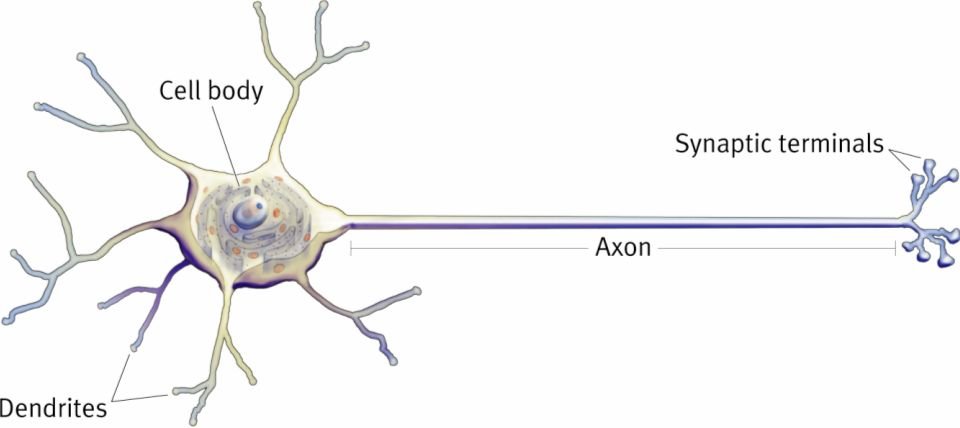
\includegraphics[]{images/neuron.jpg}
\caption[Structure of a neuron]{Structure of a neuron
(\url{http://bio3520.nicerweb.com/Locked/chap/ch03/neuron.html}).}\label{neuron-sections}
\end{figure}

In the dendrites, the neuron receives input from other nerve cells,
usually via synaptic connections (a form of chemical signal
transmission, see below). In response to an action potential of the
presynaptic cell, the synapse causes a flow of ions across the membrane
of the postsynaptic neuron. Consequently, its membrane potential changes
locally. Depending on the type of the synapse, it can either increase
(depolarization, activating input) or decrease (hyperpolarization,
inhibiting input).

This local perturbation of the membrane potential spreads through ionic
diffusion. On its way towards the soma, the electric signal mixes with
inputs that arrive at other locations in the dendrites and at slightly
different times. Summation of these signals (both spatially and
temporally) is the main function of the dendritic tree. Dendrites are
usually passive (i. e. they do not alter the incoming electric signals
or fire action potentials), but can show active behaviour in some cases
(Koch 2004, p.~428).

The electric signals from the dendrites eventually merge at the soma and
arrive at the spike initiation zone (usually located between soma and
axon). Here, the decision to fire an action potential is made. In short,
firing of a spike requires the membrane potential to be raised above a
threshold value (we will see from the dynamical systems analysis
in~\ref{dynamical-systems} that this simple concept is not really
correct, especially for some types of neurons).

Biophysically, a spike is produced by voltage-gated ion channels along
the axon (see~\ref{hodgkin-huxley-model}). In response to a sufficient
depolarization, they generate a transient flow of ions across the
membrane, which causes a short and strong depolarization (the spike).
Its shape (fig.~\ref{spike}) is always more or less equal (as described
earlier, from the dynamics point of view there are exceptions,
see~\ref{dynamical-systems}). In this sense, a spike is a discrete,
all-or-none event. Once initiated, the spike activates ion channels in
neighbouring regions of the axon and eventually spreads across its
entire length.

At its end, the axon branches out and connects to subsequent neurons via
synapses. There is no direct contact between the two cells. Instead, the
spike signal is transmitted on a chemical pathway: The synapse releases
neurotransmitters into the synaptic cleft (the space between the
neurons). These chemicals bind to receptors on the postsynaptic membrane
and cause a flow of ions across it.

\subsection{Passive Membrane Model}\label{passive-membrane-model}

For a simple neuron model, we treat the cell membrane as a purely
passive structure (i. e. we omit any active ionic currents that generate
spiking). Biologically, the membrane consists of phospholipids, which
act as a capacitance $C$ between the interior and exterior of the cell.
Also, the membrane is semipermeable to ions at any time. We can model
this behaviour by a small conductance $g_{leak}$ between the inside and
outside (or a strong resistor, respectively).

\begin{figure}
\centering
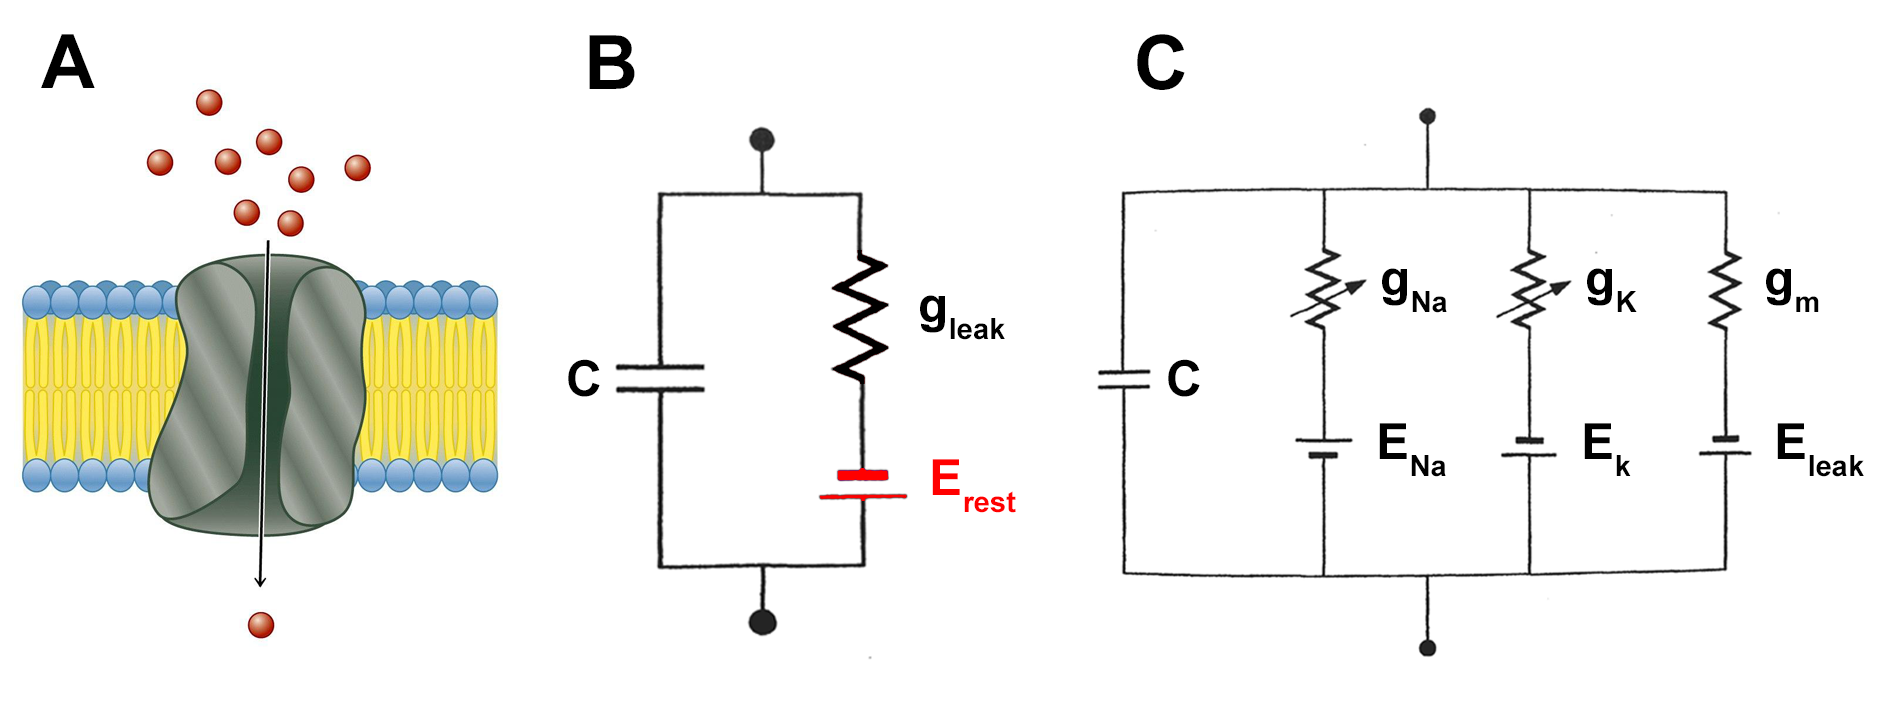
\includegraphics[]{images/circuits.png}
\caption[Modelling a neuron membrane]{Modelling a neuron membrane (bottom is intracellular, top
is extracellular). \textbf{A:} Membrane with ion channel (Horton 2006).
\textbf{B:} Passive membrane model (adapted from Koch 2004, p.~7).
\textbf{C:} Hodgkin-Huxley model (adapted from Koch 2004,
p.~345).}\label{circuits}
\end{figure}

All in all, we can represent the nerve cell as a simple RC circuit
(fig.~\ref{circuits}A without the red part). For external stimulation,
we add a current input $I$ (with opposite direction to the other
currents, in accordance with the literature). Using Kirchhoff's circuit
laws and Ohm's law, we obtain a differential equation for the membrane
potential $V$ inside the cell (Koch 2004, p.~9):
%
\begin{equation}
\label{membrane-equation}
\frac{dV}{dt} = - \frac{1}{C} (g_{leak} V - I)
\end{equation}
%
 This equation is often called membrane equation. For a temporary
current stimulus with constant amplitude, it can be solved analytically
(Koch 2004, p.~10): At the start of the current stimulus, the membrane
potential increases slowly (the capacitance ``charges''). At the end of
the current step, it decreases back to the old equilibrium value.

In this model, the membrane potential stays at zero without a current
stimulus. However, real neurons are usually slightly depolarized at rest
(between -30 mV and -90 mV, Koch 2004, p.~6). We can include this so
called resting potential by adding a DC voltage source in line with
$g_{leak}$ (red part in fig.~\ref{circuits}B). For $I$ = 0, it drives
the voltage towards $E_{rest}$. The membrane equation becomes:
%
\begin{equation}
\label{membrane-equation-rest}
\frac{dV}{dt} = - \frac{1}{C} (g_{leak} (V - E_{rest}) - I)
\end{equation}
%

\subsection{Hodgkin-Huxley Model}\label{hodgkin-huxley-model}

The Hodgkin-Huxley model adds spiking behaviour to the passive membrane
model. It was developed during the seminal work of Hodgkin and Huxley on
the squid giant axon (Hodgkin 1952) and helped to unveil many of the
biophysical mechanisms behind action potentials. Until today, it is
widely used in neuroscience (see Catterall 2012 for a recent review).

The key finding behind the Hodgkin-Huxley model is that spikes are
caused by the interplay of two ionic currents: sodium (Na) and potassium
(K). In response to a sufficient depolarization of the membrane, sodium
channels open quickly. This causes an influx of Na into the neuron,
which further depolarizes the membrane and initiates the spike. In
response to this strong depolarization, the sodium channels close and
slow potassium channels start to open. Now, K flows out of the neuron
and drives the membrane potential back to the resting potential, which
effectively ends the spike. However, due to their slow dynamics the
potassium channels do not inactivate instantaneously. Hence, the
membrane hyperpolarizes below its resting potential for a short amount
of time. During this refractory period, the neuron's excitability to
trigger a new spike is drastically lowered (Koch 2004, p.~154f).

The sodium and potassium currents ($I_{Na}$ and $I_K$) are added to the
passive membrane model as shown in fig.~\ref{circuits}C. The membrane
equation becomes:
%
\begin{equation}
\label{membrane-equation-hh}
\frac{dV}{dt} = - \frac{1}{C} (g_{leak} (V - E_{leak}) + I_{Na} + I_K - I)
\end{equation}
%
 In accordance with the literature, $E_{rest}$ from
eq.~\ref{membrane-equation-rest} was rewritten as $E_{leak}$. As
described above, the sodium and potassium currents are
voltage-dependent. They were modeled by Hodgkin and Huxley as
%
\begin{equation}
\label{currents-hh}
\begin{split}
I_{Na} = \bar{g}_{Na} m^3 h (V - E_{Na}) \\
I_{K} = \bar{g}_K n^4 (V - E_K).
\end{split}
\end{equation}
%
 Here, the strength of each ion current is mediated by the maximal
conductance ($\bar{g}_{Na}$ or $\bar{g}_K$) and a combination of the
gating variables $n$, $m$ and $h$. These dimensionless variables have
values between 0 and 1 and activate ($n$, $m$) or inactivate ($h$) the
currents. Biophysically, they can be interpreted stochastically: For
$n^4$ = 0, all potassium channels are closed; for $n^4$ = 1 they are
open (accordingly for $m^3 h$ and sodium). $E_{Na}$ and $E_K$ are the
reversal potentials for the respective ions.

The dynamics of the gating variables are voltage-dependent (i. e. the
ion channels open or close according to the current membrane potential).
They can be expressed in two equivalent ways: Either via rate constants
$\alpha_n (V)$ and $\beta_n (V)$ as in
%
\begin{equation}
\label{rates-hh}
\frac{dn}{dt} = \alpha_n (V) n + \beta_n (V) (1 - n).
\end{equation}
%
 or via a steady-state value $n_{\infty}$ and a time constant $\tau_n$
as in
%
\begin{equation}
\label{steady-tau-hh}
\frac{dn}{dt} = \frac{n_{\infty}(V) - n}{\tau_n(V)}.
\end{equation}
%
 The functions for rate constants, steady-state values and time
constants depend on the specific model properties. Often, they are
expressed as sigmoid functions. Fig.~\ref{spike} shows a spike simulated
by the original Hodgkin-Huxley. Today, many simulations use variations
of this model, for example with additional ion channels.

\begin{figure}
\centering
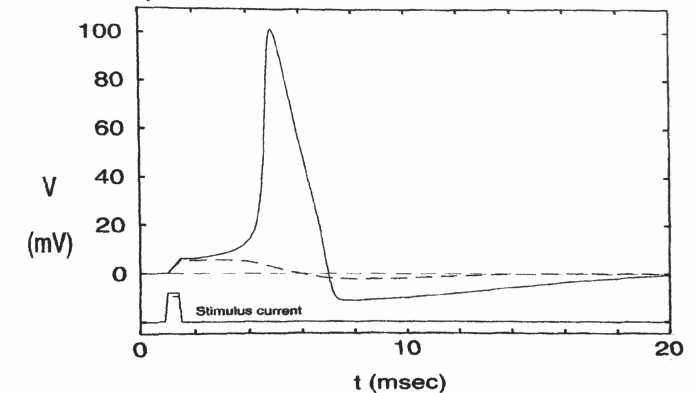
\includegraphics[width=0.600\hsize]{images/Koch_2004_p_150.png}
\caption[Membrane potential of the Hodgkin-Huxley model]{Membrane potential (top) of the Hodgkin-Huxley model
in response to a sub- and suprathreshold current stimulus (bottom; Koch
2004, p.~150).}\label{spike}
\end{figure}

\subsection{Compartmental Models}\label{compartmental-models}

The models above treat the neuron as a point-like structure: Each state
variable is represented by a single value. For example, the membrane
potential $V$ is equal across the entire neuron (it is isopotential). In
a real neuron however, the membrane potential differs across the complex
morphology (see~\ref{neuron-structure}).

To incorporate this morphological heterogeneity, Rall (1989) modeled the
neuron as a set of cables (cylinders of finite length). For a passive
cable without stimulus, the membrane potential at a position $x$ is
described by the cable equation (Koch 2004, p.~30):
%
\begin{equation}
\label{cable-equation}
\tau \frac{\partial V}{\partial t} = \lambda^2 \frac{\partial^2 V}{\partial x^2} - (V - E_{rest})
\end{equation}
%
 Here, $\tau$ and $\lambda$ are parameters based on the properties of
the neuron. In numerical simulations, the positions need to be
discretised. For this purpose, each cable is divided into several
isopotential compartments. Today, most simulations of morphologically
realistic neurons use compartmental models.

As the model used in this thesis is isopotential
(see~\ref{mn1-ib-model}), the details of multi-compartmental models will
not be discussed. For an introduction to the topic, see Koch 2004
(pp.~25-84).

\section{Dynamical Systems in Neuroscience}\label{dynamical-systems}

The theory of dynamical systems was shaped in large parts by the work of
Poincare in the 19th century. Initially, it was applied to problems in
engineering and physics. Today, dynamical systems analysis is used in a
broad range of disciplines that employ modelling and simulation
(Strogatz 1994, pp.~2-4). The topic was first applied to neuroscience in
a paper by Rinzel (1989).

Strogatz 1994 gives a general introduction to dynamical systems. A more
comprehensive discussion can be found in Kuznetsov 1998, for example.
The application of dynamical systems theory to neuroscience is presented
in Izhikevich 2000 and Izhikevich 2007.

\subsection{Definition: Dynamical
System}\label{definition-dynamical-system}

A dynamical system consists of:

\begin{enumerate}
\def\labelenumi{\arabic{enumi}.}
\itemsep1pt\parskip0pt\parsep0pt
\item
  A set of variables that completely describe the current state of the
  system.
\item
  A set of laws that describe how these state variables evolve with
  time.
\end{enumerate}

A dynamical system can be continuous in time (then the laws are
differential equations) or discrete (then the laws are iterated maps or
difference equations). In the following, only continuous systems will be
described (for discrete dynamical systems see for example Strogatz 1994,
pp.~348-388). The dimension of a dynamical system is equal to the number
of its state variables.

One example for a (continuous) dynamical system in neuroscience is the
original Hodgkin-Huxley model described in~\ref{hodgkin-huxley-model}:
The state variables are the membrane potential $V$ and the gating
variables $n$, $m$ and $h$. The laws are the differential equations for
these variables ($dV/dt$, $dn/dt$, $dm/dt$, $dh/dt$). The system is
four-dimensional.

\subsection{Elements of the Phase
Space}\label{elements-of-the-phase-space}

The central concept of dynamical systems analysis is the phase space (or
state space). It is made up of all possible states of the dynamical
system (i. e. all possible combinations of state variables). For a
two-dimensional system with state variables $x$ and $y$, the phase space
is simply the Euclidean plane with axes $x$ and $y$.

The current state of a dynamical system correlates to a unique point in
the phase space. The differential equations of the system describe how
this state changes, and therefore how its location in phase space
changes. The equations can be visualised as a vector field in the phase
space, which ``pushes'' the state of the system around. The line that
connects subsequent points is called trajectory or orbit (Kuznetsov
1998, p.~8).

Most phase spaces contain several special elements (for example
equilibrium points or limit cycles) that attract or repel neighboring
trajectories. These elements widely determine the possible trajectories
of the system, and thus its behaviour. Together, they make up the so
called phase portrait (Strogatz 1994, p.~19).

\subsubsection{Equilibria}\label{equilibria}

Equilibria (or fixed points) are those points of the phase space at
which all differential equations vanish. If a trajectory is at an
equilibrium point, it will not move away from it (unless the system is
perturbed). An equilibrium can be stable (all neighboring trajectories
move towards it) or unstable (at least some neighboring trajectories
move away from it). In neuron models, stable equilibria represent silent
behaviour.

The stability of an equilibrium can be determined analytically. For this
purpose, we will linearize the differential equations of the system in a
small region around the equilibrium (Strogatz 1994, pp.~150-151). We
take a two-dimensional system
%
\begin{equation}
\label{stability-system}
\begin{split}
\dot{x} = f(x, y) \\
\dot{y} = g(x, y)
\end{split}
\end{equation}
%
 with a fixed point $(x_0, y_0)$. This implies
%
\begin{equation}
\label{stability-implication}
f(x_0, y_0) = g(x_0, y_0) = 0.
\end{equation}
%
 Now, we want to see how the state of the system at a point close to the
equilibrium evolves. To describe this state, we introduce local
coordinates
%
\begin{equation}
\label{stability-linearization}
\begin{split}
u = x - x_0 \\
v = y - y_0.
\end{split}
\end{equation}
%
 Taking the time derivative and applying a Taylor series expansion
yields
%
\begin{equation}
\label{stability-taylor}
\begin{split}
\dot{u} = \dot{x} = f(x_0 + u, y_0 + v) = u \frac{\partial f}{\partial x} + v \frac{\partial f}{\partial y} + \mathcal{O}(u^2, v^2, uv) \\
\dot{v} = \dot{y} = g(x_0 + u, y_0 + v) = u \frac{\partial g}{\partial x} + v \frac{\partial g}{\partial y} + \mathcal{O}(u^2, v^2, uv).
\end{split}
\end{equation}
%
 As $u$ and $v$ are small, the quadratic terms can be omitted. We
rewrite the time evolution of the local state in vector form:
%
\begin{equation}
\label{stability-vector}
\begin{aligned}
\binom{\dot{u}}{\dot{v}} = \underbrace{
\begin{pmatrix}
\frac{\partial f}{\partial x}&\frac{\partial f}{\partial y} \\
\frac{\partial g}{\partial x}&\frac{\partial g}{\partial y} 
\end{pmatrix}
}_{=: J} \binom{u}{v}
\end{aligned}
\end{equation}
%
 Here, $J$ is the Jacobian matrix of the system. Evaluated at an
equilibrium, it describes how a state close to that equilibrium evolves
with time. To infer the stability of the equilibrium, we can simply
analyse the eigenvalues of $J$: If an eigenvalue is negative, all
trajectories in the direction of the respective eigenvector will move
towards the equilibrium. If the eigenvalue is positive, they will move
away from it. Hence, the equilibrium is stable if all eigenvalues of the
Jacobian have negative real part and unstable if at least one eigenvalue
has positive real part (Kuznetsov 1998, p.~22).

This technique of linearization and eigenvalue analysis can be easily
extended to systems with $n$ dimensions. Then, the Jacobian $J$ is a
$n \times n$ matrix and has $n$ eigenvalues. The definition of stability
remains the same.

Equilibria can be further classified (following the nomenclature in
Izhikevich 2007, p.~104, and Kuznetsov 1998, p.~49): As nodes (all
eigenvalues real and same sign), saddles (all eigenvalues real and at
least two eigenvalues with opposite sign), and foci (at least two
eigenvalues complex-conjugate). In the latter case, trajectories close
to the equilibrium oscillate around it (due to the imaginary part of the
eigenvalues).

Fig.~\ref{equilibria-classification} depicts typical trajectories and
eigenvalues for all possible equilibria. Additionally, there are some
rare types of equilibria which cannot be analysed via linearization (the
quadratic terms in eq.~\ref{stability-taylor} do not vanish for them).
For a discussion of these borderline cases see Strogatz 1994 (pp.~151,
133-137).

\begin{figure}
\centering
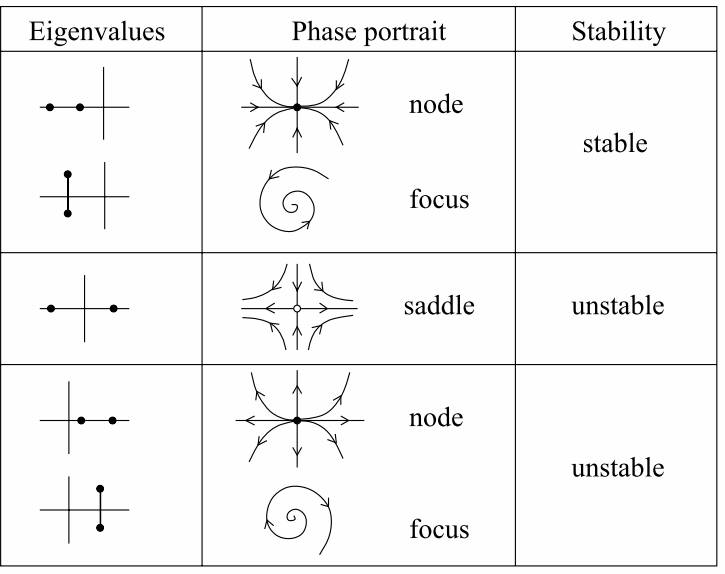
\includegraphics[]{images/Kuznetsov_1998_p_49_adapted.png}
\caption[Classification of equilibria in the phase plane]{Classification of equilibria in the phase plane (adapted
from Kuznetsov 1998, p.~49).}\label{equilibria-classification}
\end{figure}

\subsubsection{Limit Cycles}\label{limit-cycles}

Limit cycles are isolated periodic solutions of a dynamical system (i.
e. neighboring solutions in phase space are not periodic). If a
trajectory is on a limit cycle, it will stay on it and keep oscillating
(unless the system is perturbed). Like all periodic solutions, limit
cycles need phase spaces with at least two dimensions. A limit cycle can
be stable (neighboring trajectories spiral towards it), unstable (they
spiral away from it) or - in rare cases - half-stable (trajectories
inside the limit cycle spiral towards it, trajectories outside spiral
away, or vice versa). In neuron models, stable limit cycles correspond
to repeated spiking.

Unlike with equilibria, there is no straightforward, analytical method
to determine whether a given dynamical system has a limit cycle or not,
and how its stability and shape is. For a discussion of some techniques
to investigate these questions, see Strogatz 1994 (pp.~199-215).

\subsection{Bifurcations}\label{bifurcations}

As the parameters of a dynamical system are altered, its phase portrait
changes. Most of these changes are quantitative (e. g. equilibria move
to new values, limit cycles change their shape), but some are
qualitative (equilibria or limit cycles appear, disappear or change
stability). These qualitative changes of the phase portrait are called
bifurcations. As they substantially impact the possible trajectories,
they usually lead to qualitatively different behaviours. For example, if
the current stimulus ($I$ in eq.~\ref{membrane-equation-hh}) is
increased, bifurcations can switch neuron models from silent to spiking
behaviour.

Bifurcations are classified according to the number of parameters
involved: Codimension-1 bifurcations occur if a single parameter of the
system is varied. In contrast, codimension-2 bifurcations require two
parameters to be changed simultaneously (Izhikevich 2007, p.~159).

\subsubsection{Bifurcations of Codimension
1}\label{bifurcations-of-codimension-1}

For phase spaces with at least two dimensions, there are six important
types of codimension-1 bifurcations. Some of them involve only
equilibria, some involve only limit cycles, and some involve both. In
three and more dimensions, there are some additional bifurcations of
limit cycles. However, they are not substantial for basic neuron
behaviour (for details about them see Izhikevich 2007, pp.~190-192). The
six important bifurcations are outlined below. Common alternative names
are given in brackets. Here, the bifurcations are described in the
direction of 1) stable equilibria disappearing and 2) stable limit
cycles emerging. This is the typical behaviour at the onset of spiking
in neurons. However, all bifurcations can also occur in the opposite
direction (Izhikevich 2007, p.~209). Fig.~\ref{bifurcations-phase-plane}
shows the phase portrait before, during and after each bifurcation.

The following two bifurcations destroy a stable equilibrium, without
involving a stable limit cycle. In the phase space, a stable equilibrium
corresponds to negative eigenvalues of the Jacobian
(see~\ref{equilibria}). The bifurcations of equilibria affect the
stability (or existence) of the equilibrium. Therefore, at least one
eigenvalue of the Jacobian crosses the imaginary axis and become
positive.

\begin{itemize}
\item
  \emph{Saddle-node} (fold, limit point): A saddle and a node merge and
  vanish. At the bifurcation, one real eigenvalue crosses the imaginary
  axis.
\item
  \emph{Subcritical Hopf}: An unstable limit cycle shrinks to a stable
  equilibrium, which becomes unstable. The two complex conjugate
  eigenvalues cross the imaginary axis.
\end{itemize}

The following two bifurcations destroy a stable equilibrium and create a
stable limit cycle in the same process:

\begin{itemize}
\item
  \emph{Saddle-node on invariant circle} (SNIC, SLNC): Normal
  saddle-node bifurcation of equilibria that occurs on an invariant
  circle (i. e. any trajectory that starts on the circle ends on it).
  When the equilibria vanish, the circle becomes a stable limit cycle.
\item
  \emph{Supercritical Hopf}: A stable limit cycle appears from a stable
  equilibrium, which becomes unstable. The two complex conjugate
  eigenvalues cross the imaginary axis.
\end{itemize}

The following two bifurcations involve only limit cycles:

\begin{itemize}
\item
  \emph{Fold limit cycle} (saddle-node of limit cycle, saddle node of
  periodic orbits): A stable and unstable limit cycle appear together
  (``out of nowhere'') and move away from each other.
\item
  \emph{Homoclinic} (saddle-homoclinic orbit): A homoclinic orbit to a
  saddle becomes a limit cycle (the saddle remains). Like the Hopf
  bifurcation, this can be divided into a supercritical case (limit
  cycle is stable) and a subcritical case (limit cycle is unstable). For
  neuroscience, only the supercritical case is important. Thus, we
  always refer to this case from now on (following the nomenclature in
  Izhikevich 2007, p.~185).
\end{itemize}

\begin{figure}
\centering
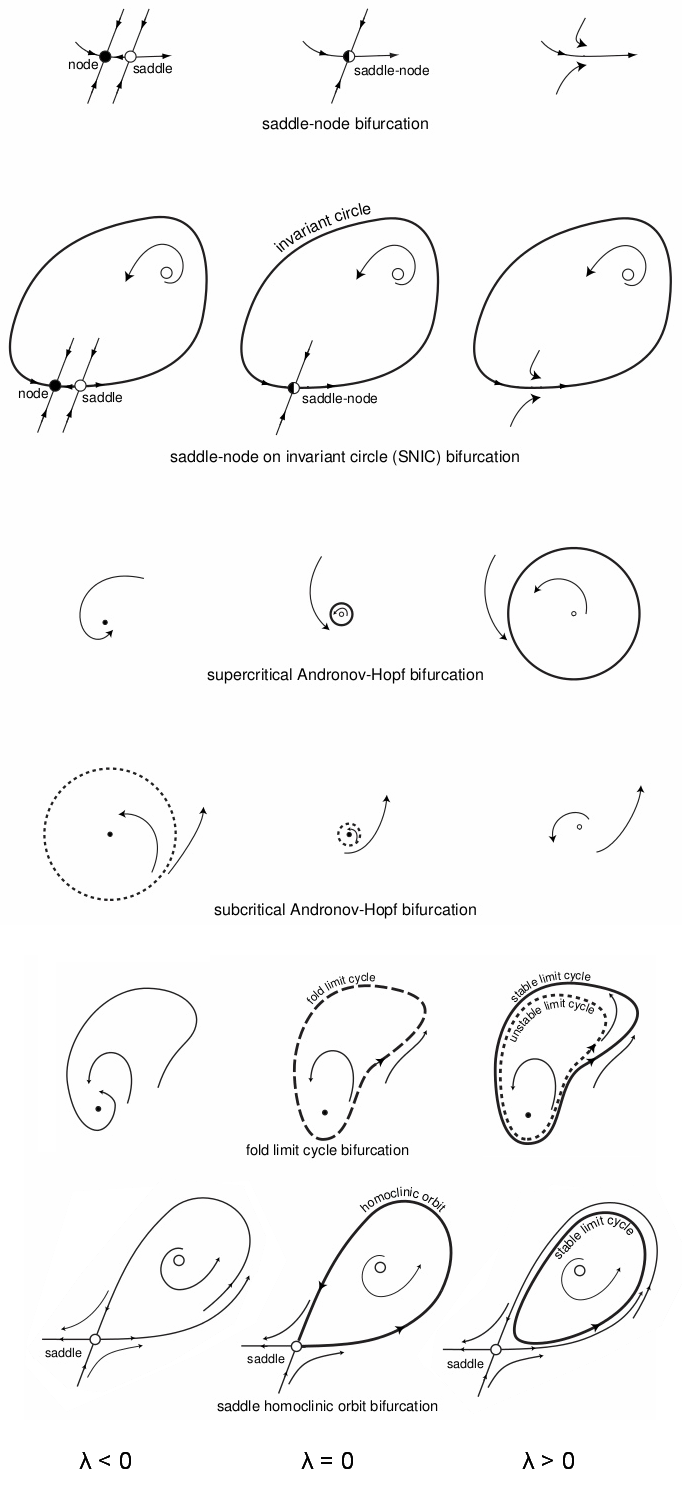
\includegraphics[width=0.600\hsize]{images/bifurcations.png}
\caption[Phase plane before, during and after a bifurcation]{Phase plane before, during and after a bifurcation at
$\lambda$ = 0 (adapted from Izhikevich 2007,
pp.~206-207).}\label{bifurcations-phase-plane}
\end{figure}

\subsubsection{Bifurcations of Codimension
2}\label{bifurcations-of-codimension-2}

Bifurcations of codimension 2 occur if two parameters of the system are
changed concurrently. In neuroscience, they usually switch the complete
behaviour and computational properties of a neuron. There are many
different types of codimension-2 bifurcations. Three important examples
are outlined below, for a complete overview see Kuznetsov 1998
(pp.~293-390).

\begin{itemize}
\item
  \emph{Cusp}: Two saddle-node points merge and vanish.
\item
  \emph{Bogdanov-Takens}: Simultaneous saddle-node and Hopf bifurcation.
  Two complex conjugate eigenvalues cross the imaginary axis through the
  origin. Hence, their imaginary part vanishes and they become real.
  Furthermore, a homoclinic bifurcation always appears near the
  Bogdanov-Takens bifurcation (Izhikevich 2007, p.~195).
\item
  \emph{Bautin} (generalized Hopf): Simultaneous Hopf and fold limit
  cycle bifurcation. The Hopf bifurcation changes from supercritical to
  subcritical (or vice versa).
\end{itemize}

\subsection{Neurons as Dynamical
Systems}\label{neurons-as-dynamical-systems}

Typical neuron models (like the Hodgkin-Huxley model
in~\ref{hodgkin-huxley-model}) are dynamical systems. Analysing their
phase space can yield insight about the behaviour of the neuron.
Specifically, we are usually interested in how a neuron reacts to
current input (which may be caused either by synaptic activation or by
artificial stimulation). To investigate this question, we look at the
changes of the phase portrait as we alter the stimulating current $I$
(eq.~\ref{membrane-equation-hh}).

Usually, for low values of $I$ the neuron has a stable equilibrium,
which corresponds to silent behaviour. A transient stimulus offsets the
trajectory from this equilibrium: If it is weak, the trajectory decays
right back towards the equilibrium; if it is strong enough, it sends the
trajectory temporarily on a circle-like structure, which corresponds to
a single spike. If the stimulating current $I$ is raised, the neuron
typically undergoes one or two bifurcations of codimension 1. These
bifurcations destroy the stable equilibrium and create a stable limit
cycle, which corresponds to (repeated) spikes. Therefore, the neuron
transitions from silent to spiking behaviour. Typical combinations of
bifurcations at this transition are shown in
fig.~\ref{bifurcation-combinations}. At very high values of $I$,
additional bifurcations may cause the neuron to stop spiking and switch
back to silent behaviour.

\begin{figure}
\centering
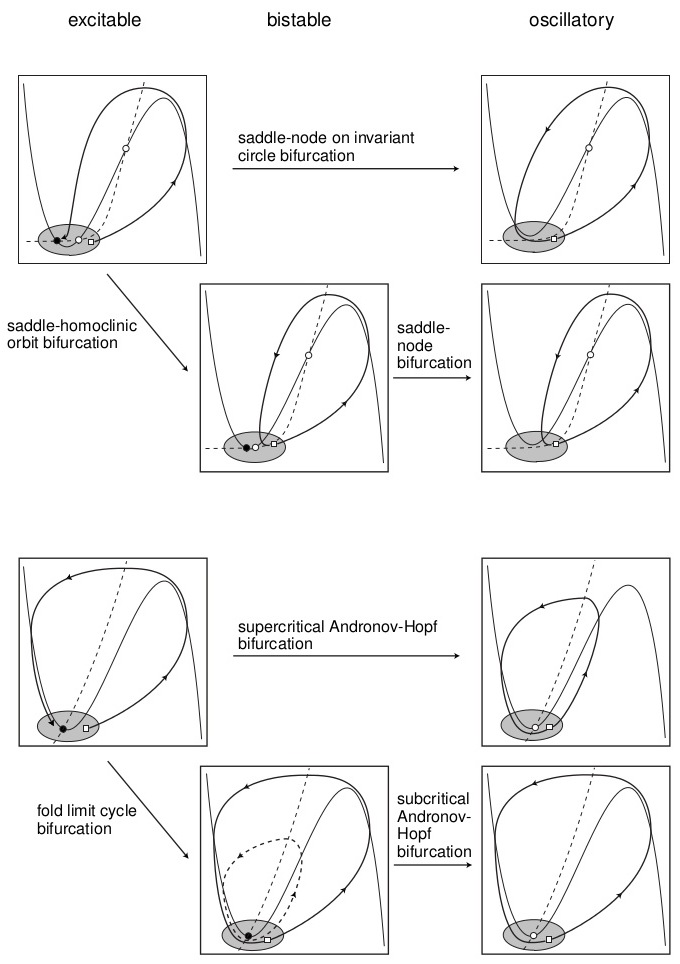
\includegraphics[]{images/bifurcation-combinations.jpg}
\caption[Possible combinations of bifurcations at the onset of
spiking]{Possible combinations of bifurcations at the onset of
spiking (transition from silent to spiking behaviour; Izhikevich
2007, p.~217).}\label{bifurcation-combinations}
\end{figure}

As outlined, bifurcations play a central role in neuroscience. They are
the dynamical mechanisms behind the onset of spiking (and all other
transitions of behaviour). Furthermore, neurons are only excitable (i.
e. they are able to fire spikes) because they are close to such
bifurcations (Izhikevich 2007, p.~215). The types of bifurcations that a
neuron undergoes widely determine its behavioural and computational
properties (Izhikevich 2007, p.~11). Fig.~\ref{bifurcation-properties}
gives an overview of such properties and the associated bifurcations.
Some of these concepts are described in more detail below.

\begin{figure}
\centering
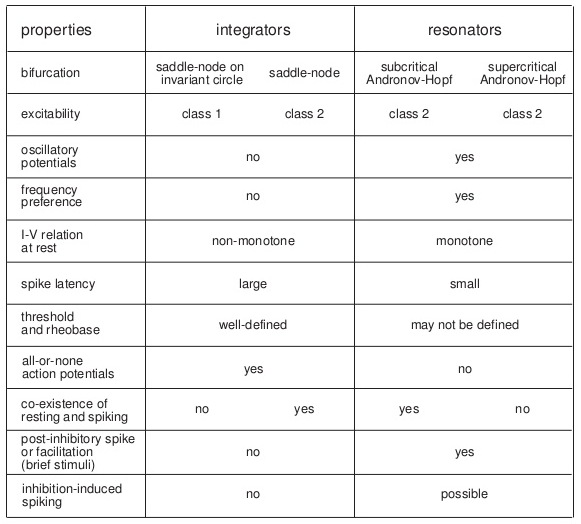
\includegraphics[width=0.700\hsize]{images/Izhikevich_2007_p_230.jpg}
\caption[Neuron properties associated with the bifurcation at the
onset of spiking]{Neuron properties associated with the bifurcation at the
onset of spiking (Izhikevich 2007,
p.~230).}\label{bifurcation-properties}
\end{figure}

\subsubsection{Threshold}\label{threshold}

Simple descriptions of neurons often introduce the concept of a voltage
threshold: If the membrane potential of the neuron rises above this
value (at the spike initiation zone), an action potential is fired
(see~\ref{neuron-structure}). However, from the dynamical point of view
the decision to fire a spike or not depends not only on the membrane
potential, but on the state of the neuron in the phase space (and
therefore on all state variables).

Neurons with saddle-node bifurcations (on or off the limit cycle) at the
onset of spiking show a threshold-like behaviour: Before the
bifurcation, their phase portrait contains a saddle. Its stable manifold
(i. e. the line of trajectories that move towards the saddle) serves as
a separatrix between the rest state (stable equilibrium) and a spike
(circle-like structure). A transient current pulse can push the
trajectory from the stable equilibrium across this separatrix and cause
a spike (Izhikevich 2007, pp.~238-239). However, the threshold is not a
single value of the membrane potential, but a manifold of the phase
space. In contrast, neurons with Hopf bifurcations at the onset of
spiking lack a clear threshold behaviour. Their phase space does not
contain a separatrix, and the stable equilibrium is a focus. Therefore,
they usually fire in response to repeated stimulation, which brings the
trajectory away from the focus (Izhikevich 2007, pp.~240-241).

\subsubsection{Firing Rate and Excitability Class}\label{excitability}

Tonic spiking of a neuron is caused by oscillations on a stable limit
cycle. The properties of this cycle determine the firing rate (i. e. the
frequency of spiking) and the spike amplitude. Depending on the type of
bifurcation of the limit cycle, these values follow specific scaling
laws, which are given in Strogatz 1994 (p.~264) or Izhikevich 2007
(p.~178).

For the firing rate, two types of behaviour can be distinguished at the
onset of spiking. These are described by the classification of
excitability from Hodgkin (1948): Class 1 neurons can spike at
arbitrarily low frequencies. At the onset of spiking, their firing rate
increases continuously from zero to higher values
(fig.~\ref{hodgkin-classification} left). In contrast, class 2 neurons
start spiking at non-zero frequencies. Their firing rate shows a
discontinuous jump at the onset of spiking
(fig.~\ref{hodgkin-classification} right). Which class a neuron belongs
to is determined by the bifurcation at the onset of spiking: A
saddle-node on invariant circle bifurcation causes class 1 excitability,
all other codimension-1 bifurcations cause class 2 excitability.

\begin{figure}
\centering
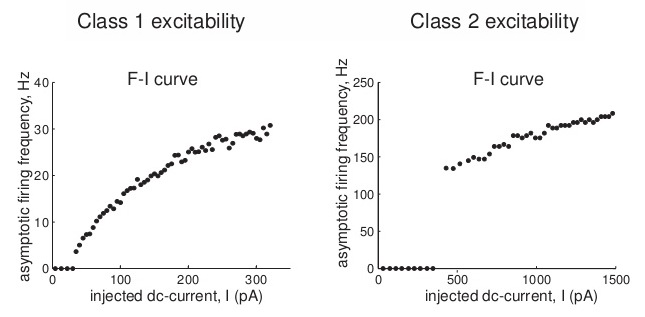
\includegraphics[width=0.800\hsize]{images/Izhikevich_2007_p_219.jpg}
\caption[Firing rates for neurons with class 1 and 2 excitability]{Firing rates for neurons with class 1 and 2 excitability
(Izhikevich 2007, p.~219).}\label{hodgkin-classification}
\end{figure}

Hodgkin's classification of excitability describes the transition from
silent to spiking behaviour (i. e. if the stimulus current is raised).
However, this transition is not necessarily governed by the same
bifurcation as the transition in the other direction (i. e. if the
stimulus current is lowered). Izhikevich 2007 (p.~228) suggests a
complementary classification for this situation: A neuron is class 1
spiking if it shows an arbitrarily low firing rate at the transition
from spiking to silent behaviour, and class 2 spiking if it has a
non-zero firing rate.

\subsubsection{Bistability}\label{bistability}

At the onset of spiking, a neuron can be bistable, i. e. it can be
silent or spike repeatedly for the same current input. This behaviour
requires the coexistence of a stable equilibrium and a stable limit
cycle. Therefore, these two elements have to be created/destroyed by two
separate bifurcations. Usually, the system first undergoes a bifurcation
that creates a stable limit cycle. Then (i. e. for a stronger current
stimulus), a second bifurcation destroys the stable equilibrium.
Bistability occurs for current stimuli between these two bifurcations.
Possible combinations of bifurcations for this situation are shown in
fig.~\ref{bifurcation-combinations} (second and fourth row from the
top). If a neuron is bistable, it can be switched from silent to spiking
behaviour via short current pulses (Izhikevich 2007, pp.~10 and 13) or
noisy current input (Izhikevich, p.~13).

\subsubsection{Subthreshold
oscillations}\label{subthreshold-oscillations}

If the rest state of a neuron is a focus, it can show subthreshold
oscillations: In response to a small current input (that does not cause
a spike), the trajectory of the system oscillates around the focus while
it settles towards it. Typically, oscillations occur in conjunction with
Hopf bifurcations.

\subsubsection{Integrators and
Resonators}\label{integrators-and-resonators}

Based on the bifurcation at the onset of spiking, neurons can be divided
into integrators (saddle-node off or on limit cycle) and resonators
(sub- or supercritical Hopf). These two neuron types show very different
computational properties. Especially, integrators fire action potentials
based on the strength of the stimulation (i. e. if the stimuli coming
from the dendritic tree sum up to a certain value). In contrast,
resonators prefer to fire if they receive multiple subsequent stimuli at
a specific resonance frequency (Izhikevich 2007, p.~229-233). Hence,
integrators and resonators serve different functions in the nervous
system (Izhikevich 2007, p.~237).

\section{\emph{Drosophila} and its
Motoneurons}\label{drosophila-and-its-motoneurons}

\emph{Drosophila melanogaster} is a species of small flies, commonly
called fruit flies or vinegar flies. In this thesis (as well as in most
available literature), the genus name \emph{Drosophila} is used
synonymously for the species name. \emph{Drosophila} is one of the most
widely used organisms in modern biology, especially in genetics and
developmental biology. Its ascent was promoted by its easy handling and
quick reproduction cycle. During the past decades, several nobel prizes
were awarded for work on \emph{Drosophila}. Its genome is completely
sequenced, and a plethora of genetic manipulations exist.

For neuroscience, \emph{Drosophila} offers a good balance between the
simplicity of its nervous system and the complexity of its behaviour.
Roughly, \emph{Drosophila} has 10\textsuperscript{5} neurons (human:
10\textsuperscript{10}) and 10\textsuperscript{7} synapses. Many (though
not all) of its neurons are identifiable (i. e. they exist in every
specimen; Olsen 2008). This relatively small nervous system creates a
range of complex cognitive abilities, such as recognizing objects,
remembering positions, or learning (Olsen 2008).

\subsection{Development and Anatomy}\label{development-and-anatomy}

\emph{Drosophila}'s reproduction cycle takes about two weeks from
hatching to hatching (at 25 °C; Müller 2006, p.~79). Initially, the egg
is contained in the ovary of the female animal. After fertilization, it
develops towards an embryo and hatches. Then, \emph{Drosophila}
undergoes three larval stages, which are separated by molting. Finally,
it turns into a pupa and initiates metamorphosis. The adult animal
emerges nine days after fertilization (Reece 2010, pp.~416-417; Müller
2006, pp.~79-81). Fig.~\ref{development-cycle} gives an overview of this
development cycle and the appearance at each stage.

\begin{figure}
\centering
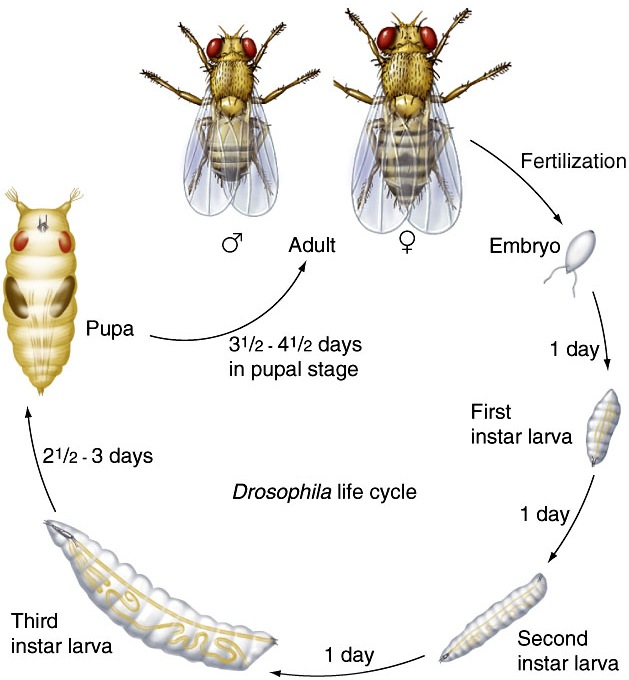
\includegraphics[width=0.600\hsize]{images/development-cycle.jpg}
\caption[Development cycle of \emph{Drosophila melanogaster}]{Development cycle of \emph{Drosophila melanogaster}
(Hartwell 2010).}\label{development-cycle}
\end{figure}

The body of \emph{Drosophila} shows a distinctive segmentation. This
characteristic is prepared in the late embryo (Müller 2006, p.~87) and
persists during the larval and adult stages. At a higher level, the body
can be divided into three parts: The head, the thorax (in the adult
animal, wings and legs are attached to this part), and the abdomen
(Campbell 2010, p.~489). The thorax can be further subdivided into three
segments (T1 to T3), the abdomen into eight segments (A1 to A8).
Fig.~\ref{larva-anatomy}A shows this segmentation at the larval stage.

Throughout its development, the body of \emph{Drosophila} undergoes many
anatomical changes. Fig.~\ref{larva-anatomy}B, C and D depict the
anatomy of the central nervous system and the somatic musculature in the
third instar larva. For details about the anatomy and development of
other systems in the body see Hartenstein 1993.

\begin{figure}
\centering
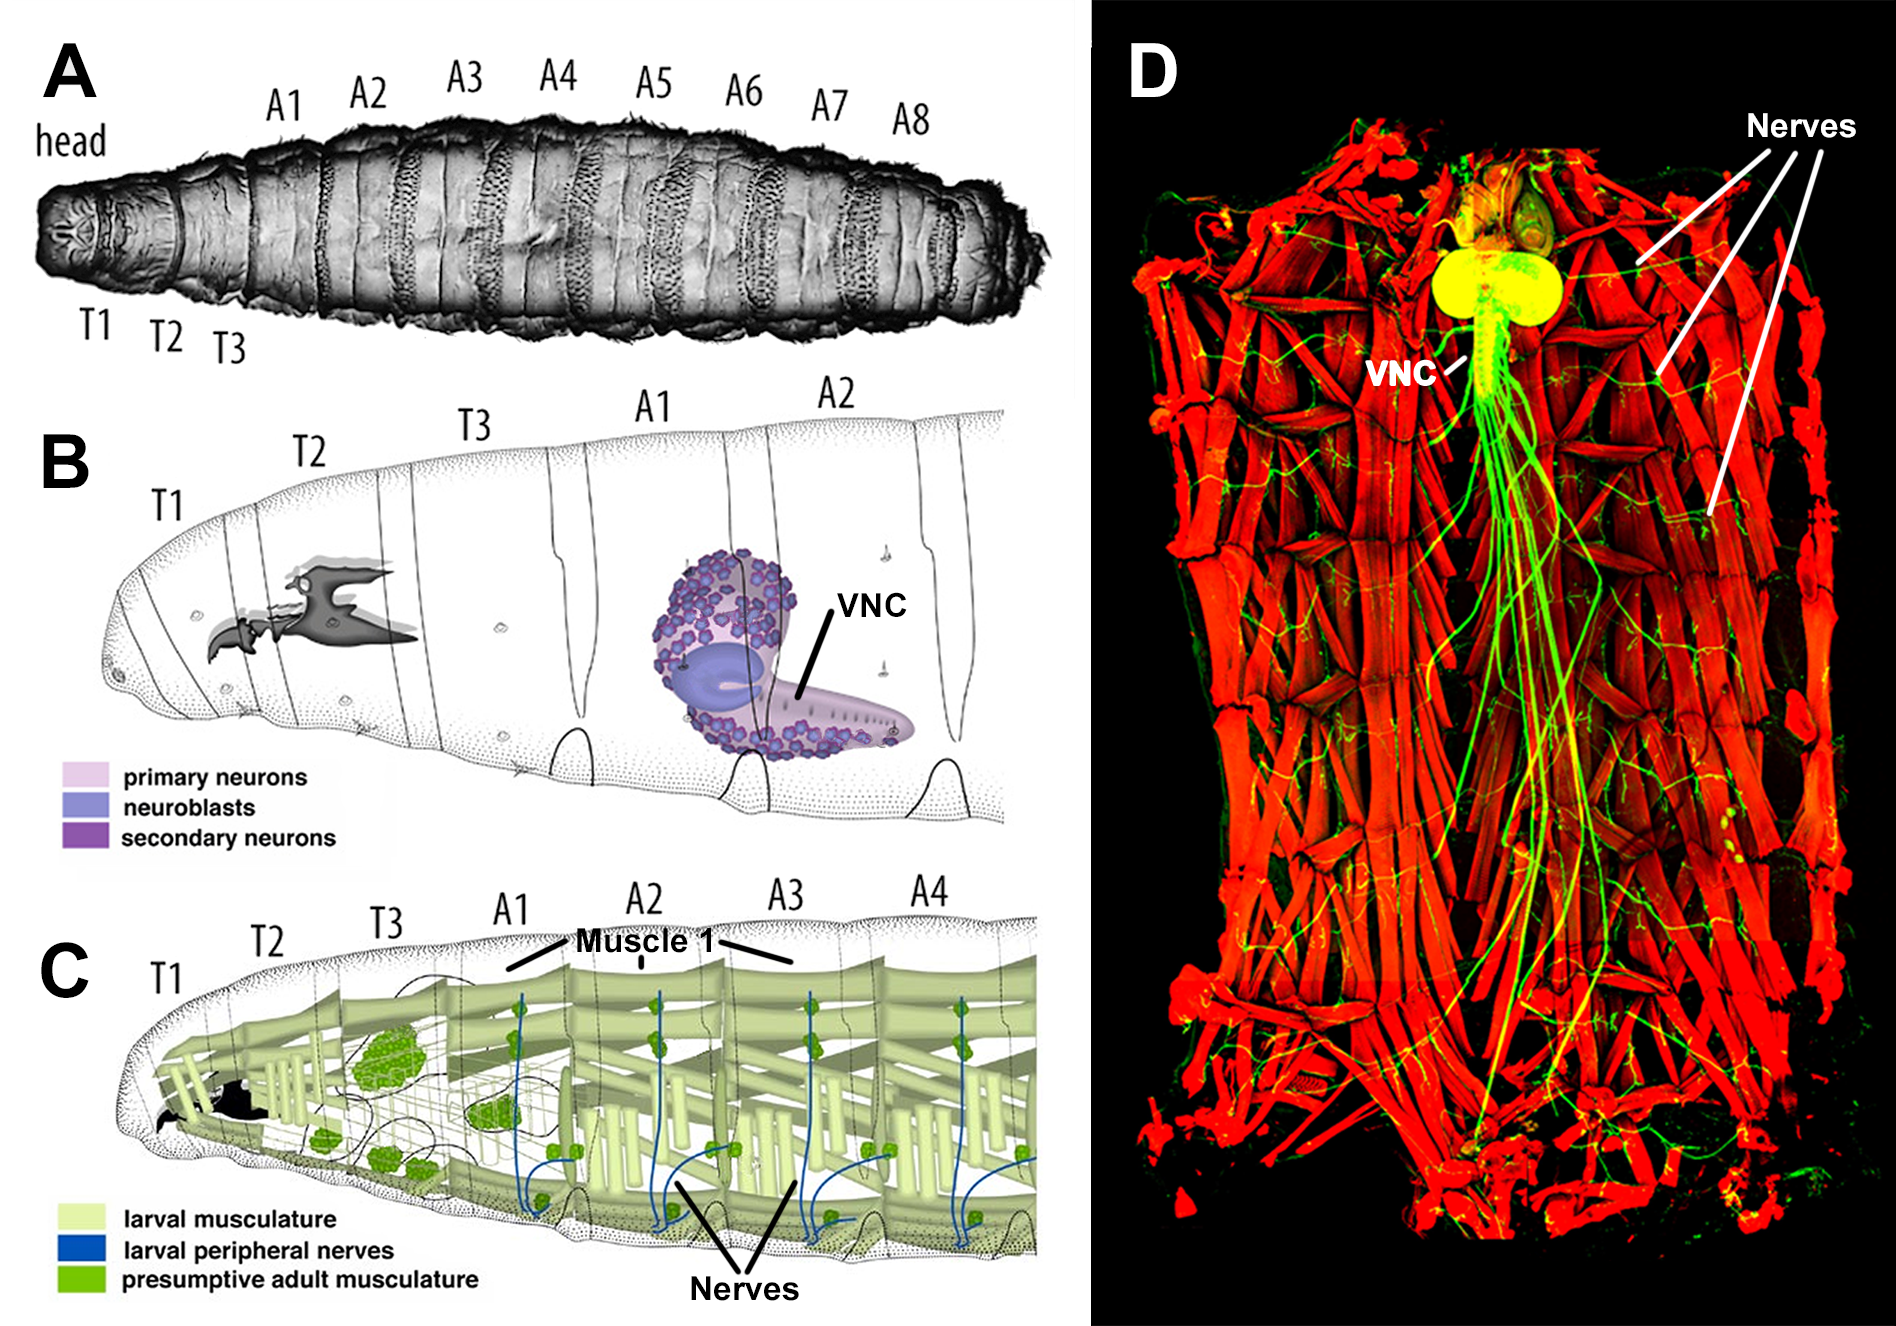
\includegraphics[]{images/larva-anatomy.png}
\caption[Anatomy of the third instar larva]{Anatomy of the third instar larva. \textbf{A:}
Segmentation
(\url{http://www.mun.ca/biology/desmid/brian/BIOL3530/DB_02/DBNDros.html}).
\textbf{B:} Central nervous system (adapted from Hartenstein 1993,
pp.~10-11). \textbf{C:} Somatic musculature (adapted from Hartenstein
1993, p.~40). \textbf{D:} Central nervous system (green) and muscles
(red) in a dissected larva (\url{https://www.ncbs.res.in/node/436}).
Muscle 1 is located on the left and right side of each
segment.}\label{larva-anatomy}
\end{figure}

\subsection{Organisation of
Motoneurons}\label{organisation-of-motoneurons}

A motoneuron is a nerve cell that innervates and controls a muscle.
Usually, it receives synaptic inputs from various sources, such as
sensory neurons and central pattern generators (CPGs; Schaefer 2010).
These neuronal circuits create rhythmic activity patterns and play a
major role for locomotion in many animals, including humans (Duysens
1998). The motoneuron integrates these signals, possibly modifies them
(Choi 2004), and sends action potentials to the subsequent muscle, which
contracts in response.

Motoneurons in \emph{Drosophila} were studied at different stages of
development: In the embryo (Goodmann 1984, Baines 1998, Sink 1991, Kim
2009), the larva (Sink 1991, Choi 2004, Kim 2009, Zwart 2013), during
metamorphosis (Consoulas 2002), and in the adult fly (Ikeda 1988).
Throughout this development, the nervous system changes significantly
(see~\ref{development-and-anatomy}). Its neuronal circuits are likely to
change as well. The following paragraphs focus on the situation in the
embryo and larva, which seem to be more or less similar in terms of
motoneuron identities and organisation (Sink 1991, Kim 2009).

\emph{Drosophila}'s motoneurons are located dorsally on the ventral
nerve cord (VNC; fig.~\ref{larva-anatomy}B and D). This structure is
symmetric along the midline (anterior-posterior axis). Each side can be
divided into a number of half-segments or hemisegments, which correlate
to the segments in the body. Each hemisegment contains a pattern of
about 400 neurons, including an estimated 38 motoneurons (Kim 2009). For
the hemisegments corresponding to abdominal body segments A2-A7, the
number of motoneurons and their relative orientation are equal (Sink
1991; Choi 2004). However, in terms of electrical properties Srinivasan
2012 reports some segmental differences of the larval motoneurons.
Fig.~\ref{motoneurons}A shows the repetition of motoneurons in the
hemisegments of the VNC. Fig.~\ref{motoneurons}B presents the
motoneurons of one hemisegment.

The axons of the motoneurons project outwards from the VNC. They lead
through dedicated nerves for each segment (fig.~\ref{larva-anatomy}C and
D and fig.~\ref{motoneurons}B) and terminate on the body wall muscles
(Sink 1991).

\begin{figure}
\centering
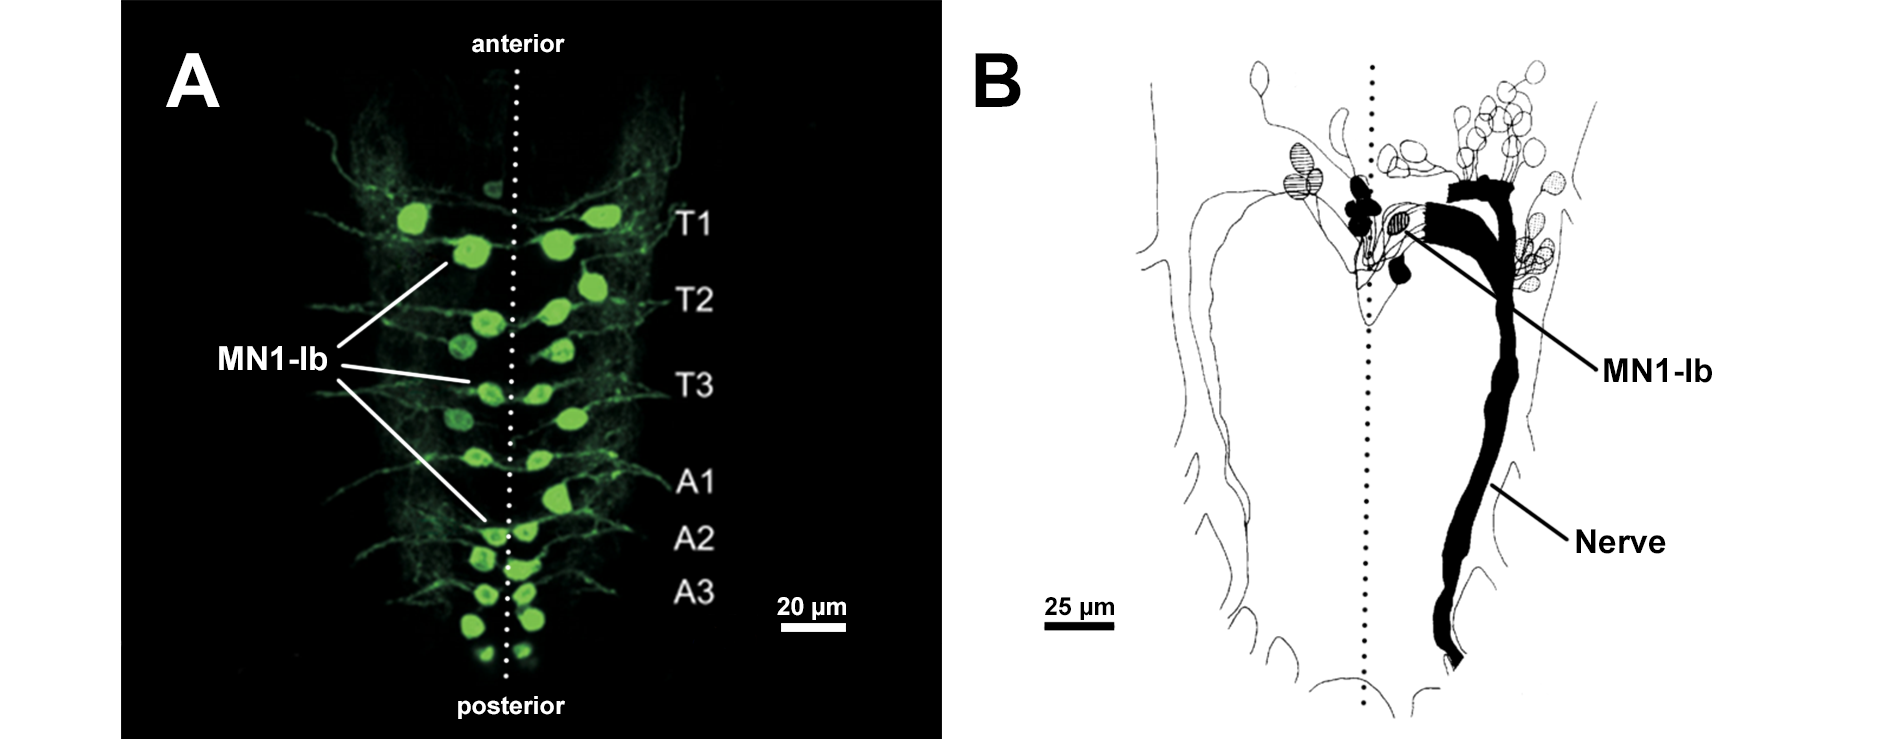
\includegraphics[]{images/motoneurons.png}
\caption[Organisation of motoneurons in the third instar larva]{Organisation of motoneurons in the third instar larva.
\textbf{A:} Segmental repetition of motoneurons in the VNC (Srinivasan
2012). \textbf{B:} Motoneurons in one hemisegment of the VNC
(corresponding to abdominal segment A6; Sink 1991).}\label{motoneurons}
\end{figure}

\subsection{The MN1-Ib Motoneuron}\label{the-mn1-ib-motoneuron}

The MN1-Ib motoneuron in \emph{Drosophila} innervates the body wall
muscle 1 (also called dorsal acute muscle 1; fig.~\ref{larva-anatomy}C
and D). Its name follows the nomenclature in Hoang 2001: MN is short for
motoneuron, 1 is the number of the target muscle, Ib is the type of the
axon terminal. The neuron is also called aCC (anterior corner cell, Sink
1991), especially in the embryo.

The positions of MN1-Ib neurons in the VNC are indicated in
fig.~\ref{motoneurons}A and B. In each hemisegment, MN1-Ib is surrounded
by various other motoneurons, which control different muscles in the
body wall. Choi 2004 describes a group of five dorsomedial neurons,
which includes MN1-Ib. This group shows a similar organisation, neuron
morphologies and electrical properties for the hemisegments
corresponding to abdominal body segments A2-A7 (Choi 2004). Also, the
group (and especially MN1-Ib) seems to be widely conserved during
development from embryo to larva (Choi 2004, Kim 2009). One other neuron
in this group (MNISN-Is) innervates the same muscle as MN1-Ib, although
its function is likely to be different. MN1-Ib seems to be the primary
contributor to motor activity of the body wall muscle 1 (Schaefer 2010).

Morphologically, the MN1-Ib neuron has two dendritic arbors, which are
highly branched (fig.~\ref{mn1-ib-morphology}; Kim 2009). Its axon
projects outwards from the ganglion through the intersegmental nerve. At
its end, it innervates the muscle with big (Ib-type) synaptic boutons
(fig.~\ref{mn1-ib-morphology}B; Choi 2004, Hoang 2001).

\begin{figure}
\centering
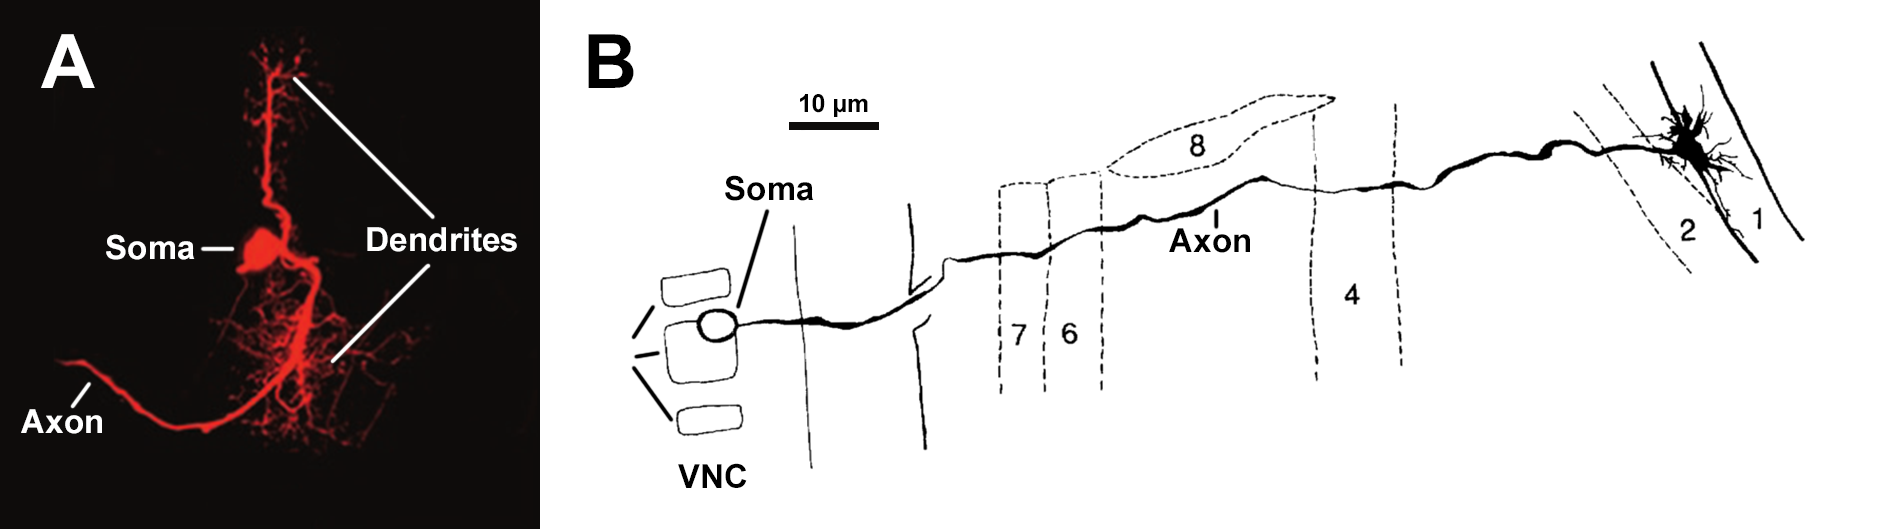
\includegraphics[]{images/MN1-Ib-morphology.png}
\caption[Morphology and connectivity of MN1-Ib]{Morphology and connectivity of MN1-Ib. \textbf{A:}
Morphology (Choi 2004). \textbf{B:} Axon and body wall muscles 1 to 8
(in the embryo; Sink 1991).}\label{mn1-ib-morphology}
\end{figure}

\chapter{Methods and Tools}\label{methods-and-tools}

\section{Availability of Data}\label{availability-of-data}

All material from this thesis is publicly available on GitHub: The LEMS
and NeuroML2 versions of the model are included in the repository of the
original model by Cengiz Günay
(\url{https://github.com/cengique/drosophila-aCC-L3-motoneuron-model}).
Additionally, they are accessible via OpenSourceBrain
(\url{http://www.opensourcebrain.org/projects/drosophila-acc-l3-motoneuron-gunay-et-al-2014}).
Everything else (simulation data, scripts for data analysis and
numerical continuation) is available in a separate repository for this
thesis
(\href{http://www.opensourcebrain.org/projects/drosophila-acc-l3-motoneuron-gunay-et-al-2014}{https://github.com/jrieke/drosophila-dynamics}).

\section{Computational Model for MN1-Ib}\label{mn1-ib-model}

In this thesis, the MN1-Ib neuron in \emph{Drosophila} was investigated.
Günay 2015 recently published three computational models for this neuron
with increasing complexity:

\begin{enumerate}
\def\labelenumi{\arabic{enumi}.}
\item
  An isopotential, single-compartmental model implemented in XPP
  (Ermentrout 2003). This model replicates the experimental f-I-curve
  and delays to first spike. However, it predicts a wrong spike
  amplitude and interspike membrane potential (Günay 2015).
\item
  A two-compartmental model (soma and axon) implemented in XPP. This
  model was published previously in Lin 2012 (with slightly different
  parameters). In contrast to the isopotential model, it replicates the
  correct spike shape.
\item
  A multi-compartmental model (based on a reconstructed neuron
  morphology) implemented in NEURON (Carnevale 2006).
\end{enumerate}

Only the first model was used for the bifurcation analysis in this
thesis (due to its small parameter and phase space). This model is an
extension of the original Hodgkin-Huxley model
(see~\ref{hodgkin-huxley-model}). It contains a leak current and four
different types of active ion currents: Fast potassium (Kf), slow
potassium (Ks), transient sodium (Na), and persistent sodium (NaP). Ca-
and Ca-gated channels were omitted because they had no effect on spike
generation in experiments. The equations for membrane potential,
currents and gating variables widely follow the formalism in
eq.~\ref{membrane-equation-hh} to~\ref{steady-tau-hh} (except for a
second inactivation gating variable for the Kf current). Steady-state
values were expressed as sigmoid functions of $V$, time constants as
sigmoid functions or constant values.

All parameters of the model are given in Günay 2015 (especially table 5
and and fig. 1F). They were obtained from several recordings, some of
which were performed on MN1-Ib itself (Günay 2015), and some on other
neurons (cultured neurons of the \emph{Drosophila} embryo (O'Dowd 1988)
and cells from \emph{Xenopus} that heterologously expressed
\emph{Drosophila}'s \emph{DmNav} gene (Lin 2009)). To keep the model at
the resting potential observed in experiments, a default holding current
of $I$ = -12 pA was applied (Günay 2015, Lin 2012).

\section{Conversion of the Model to LEMS and NeuroML2}\label{conversion}

The isopotential model of MN1-Ib was converted from XPP to NeuroML2.
NeuroML is a simulator-independent, declarative language for neuronal
modelling (Gleeson 2010, Cannon 2014). Its implementation is based on
the popular XML format (eXtensible Markup Language). The main advantages
of NeuroML over simulator-specific languages are portability (NeuroML
can be run in various simulators and converted to a range of formats),
modularity (NeuroML elements can be easily reused for other models) and
scalability (NeuroML elements can be put together to form more complex
models). See also Cannon 2007 for a discussion of modelling languages in
neuroscience.

NeuroML2 (the newest version of the NeuroML language) is based on LEMS
(Low Entropy Model Specification; Cannon 2014), a generic schema to
describe scientific models of any kind. Like NeuroML2, it is implemented
in XML. LEMS allows the user to create so called \emph{ComponentType}s,
which define parameters, state variables, differential equations etc.,
and serve as building plans for the respective \emph{Components}. For
example, the user can define a neuron model once (as a
\emph{ComponentType}) and create multiple instantiations
(\emph{Components}) for a network simulation. All objects of NeuroML2
(for example cells and channels) are implemented as such
\emph{ComponentType}s in LEMS. This allows easy extension and
modification.

The conversion of the isopotential model to NeuroML was performed in two
steps: Firstly, a pure LEMS version was created (i. e. without any of
the \emph{ComponentType}s defined by NeuroML2). A LEMS
\emph{ComponentType} for the cell was created. Then, the differential
equations and parameters of the model were transformed from XPP to the
respective elements in LEMS. Secondly, a model in native NeuroML2 was
created. The NeuroML2 elements (channels, cell, network with current
stimuli) were split up into several files to allow easier reusability.
Some custom LEMS \emph{ComponentType}s were created to account for
missing features in NeuroML2 (such as the two inactivation gates of the
Kf current, see~\ref{mn1-ib-model}).

Finally, automated tests were added to ensure the consistency of all
models. These tests check the spike times in response to a constant
current step. The results of the comparison are presented
in~\ref{consistency-of-models}.

\section{Simulation and Data
Analysis}\label{simulation-and-data-analysis}

Simulations were run in XPP (for the original model) and jnml (for the
converted LEMS and NeuroML2 models). The Euler algorithm for numerical
integration was employed at a time step of 0.001 ms. Data was exported
as text files in a CSV-style format (variables as columns, time steps as
rows).

Data analysis was performed with Python 2.7.8 for Windows 32 bit (van
Rossum 1995). All code is available in the form of interactive
Jupyter/IPython notebooks (Pérez 2007). For data handling and analysis,
the Python packages numpy (version 1.10.1) and scipy (version 0.16.1)
were used. Plots were created with matplotlib (version 1.5.0).

To calculate spike properties, simulations with constant current steps
were run for at least 500 ms. The first 100 ms and last 10 ms of each
run were omitted for analysis to prevent edge effects. From the
remaining voltage traces, spikes were detected with a threshold of -25
mV. Based on the spike times, the mean values of firing rate, spike
minima and spike maxima were calculated. In all cases, spiking was very
regular, i. e. the standard errors of spike properties were negligible.

\section{Steady-State I-V-Curve}\label{i-v-methods}

To get a first impression of equilibria in the system, the steady-state
I-V-curve was analysed. It shows the overall current flowing into the
neuron, if all gating variables are at steady state. It was calculated
with:
%
\begin{equation}
\label{i-inf}
I_{\infty}(V) = I_{\mathrm{Ks}, \infty}(V) + I_{\mathrm{Kf}, \infty}(V) + I_{\mathrm{Na}, \infty}(V) + I_{\mathrm{NaP}, \infty}(V) + I
\end{equation}
%
 Here, $I$ is the stimulating current and $I_{x, \infty}$ are the
steady-state ion currents. They were expressed as in
eq.~\ref{currents-hh}, with the gating variables replaced by their
steady-state values (see also eq.~\ref{steady-tau-hh}). Parameters
values were set as in the original model (see~\ref{mn1-ib-model}).

Calculation and plotting were performed with the same toolset as the
data analysis described in~\ref{simulation-and-data-analysis} (Python
2.7.8, numpy, matplotlib). The code is available as a Jupyter/IPython
notebook.

\section{Numerical Continuation}\label{numerical-continuation}

Bifurcations were analysed via numerical continuation. This technique
tracks the location of equilibria or limit cycles as one or more
parameters of the dynamical system are varied. Bifurcations are detected
by analysing the eigenvalues of equilibria (or multipliers for limit
cycles). For a detailed introduction to the methods behind numerical
continuation see Kuznetsov 1998 (pp.~463-535). In this thesis, the
numerical continuation software AUTO-07p was used (version 0.9.1,
installed on Windows via MinGW; Doedel 2007). The model equations were
defined in C. Parts of the code were generated from the LEMS version of
the model (see~\ref{conversion}) via jNeuroML. Scripts to run the
continuation were written for AUTO's built-in Python interface. They are
available as Jupyter/IPython notebooks.

\chapter{Results}\label{results}

\section{Consistency of the Models in XPP, LEMS and
NeuroML2}\label{consistency-of-models}

The isopotential model used for this thesis was transformed from the
original XPP format to LEMS and subsequently to NeuroML2
(see~\ref{conversion} for details). All models were run for the same
current steps with XPP and jnml, respectively. The resulting outputs
(plots of membrane potential, gating variables and currents) were
successfully checked for visual consistency. Fig.~\ref{xpp-neuroml2}
compares voltage traces from the XPP and NeuroML2 model for a constant
current step.

The simulation run shown in this figure was also analysed numerically:
Spike times were detected via a voltage threshold of -25 mV and
compared. The spike times of the LEMS model agreed completely with the
XPP model. The NeuroML2 version showed some slight deviations (maximum
0.601 ms). However, this effect was attributed to numerical errors,
because the deviations decreased when the simulation was run at a lower
time step.

\begin{figure}
\centering
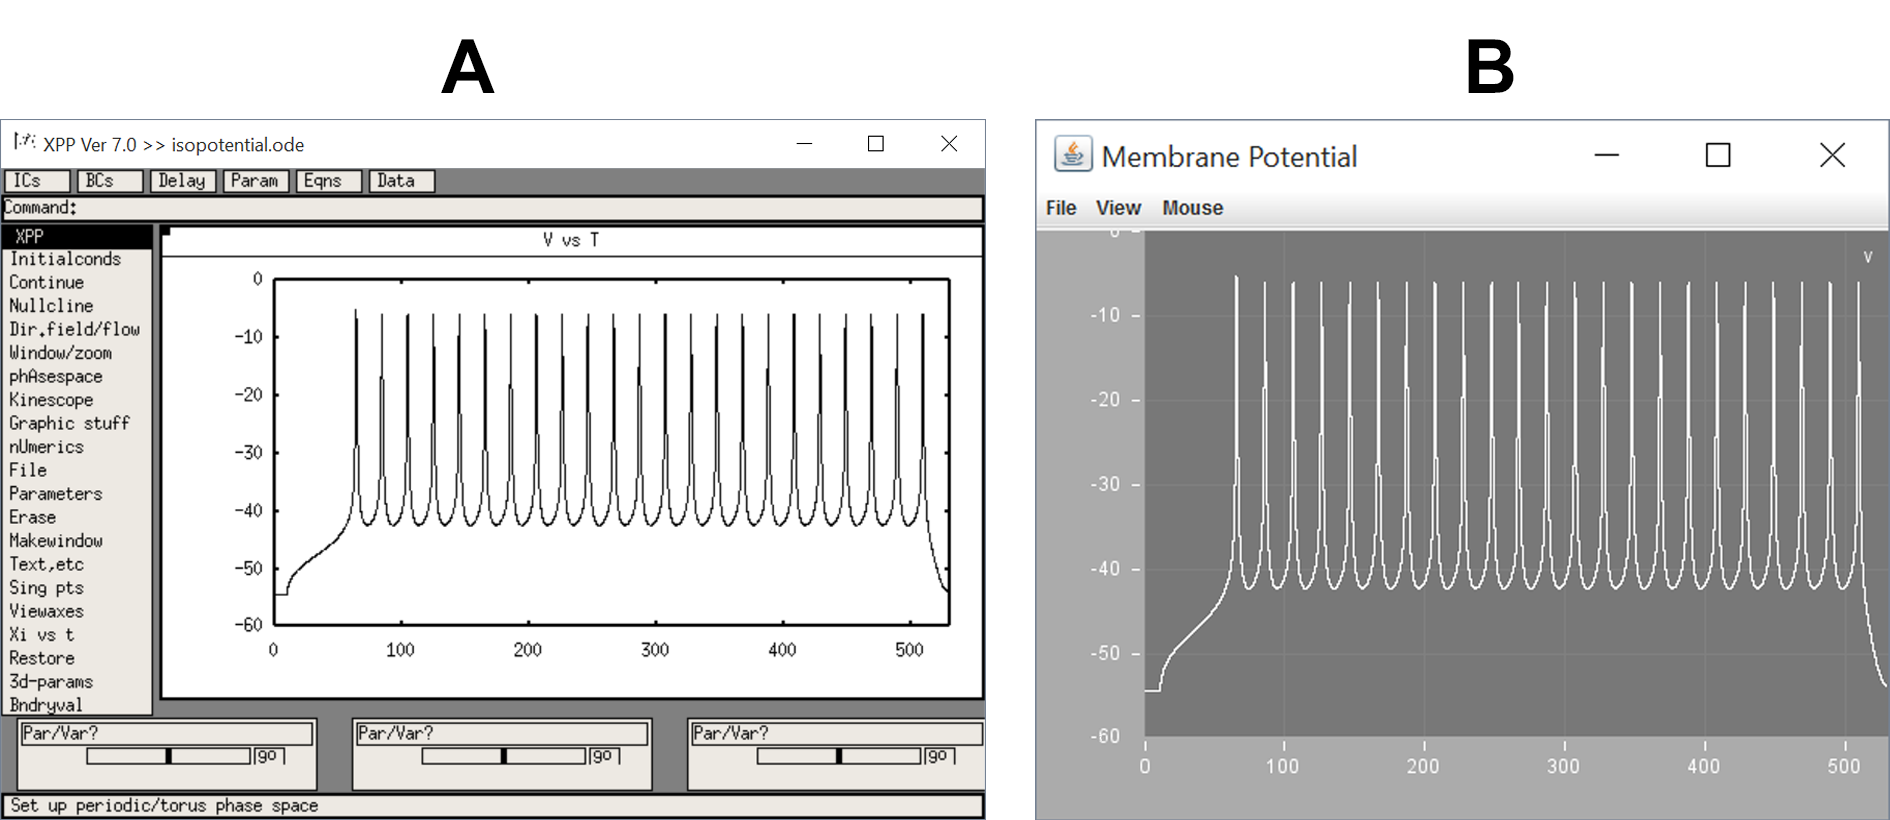
\includegraphics[]{images/xpp-neuroml2.png}
\caption[Screenshots of the same simulation run in XPP and jnml/NeuroML2]{Screenshots of the same simulation run in XPP (\textbf{A})
and jnml/NeuroML2 (\textbf{B}). Current step of 0 pA for 500
ms.}\label{xpp-neuroml2}
\end{figure}

\section{Model Behaviour in
Simulations}\label{model-behaviour-in-simulations}

To characterize the behaviour of the MN1-Ib model, simulations were run
with constant current steps. Depending on the strength of the stimulus,
the neuron showed different types of silent and spiking behaviour.
Spiking properties (firing rate, spike amplitude, delay to first spike)
were calculated from the voltage traces.

\subsection{Qualitative Behaviour}\label{qualitative-behaviour}

\begin{figure}
\centering
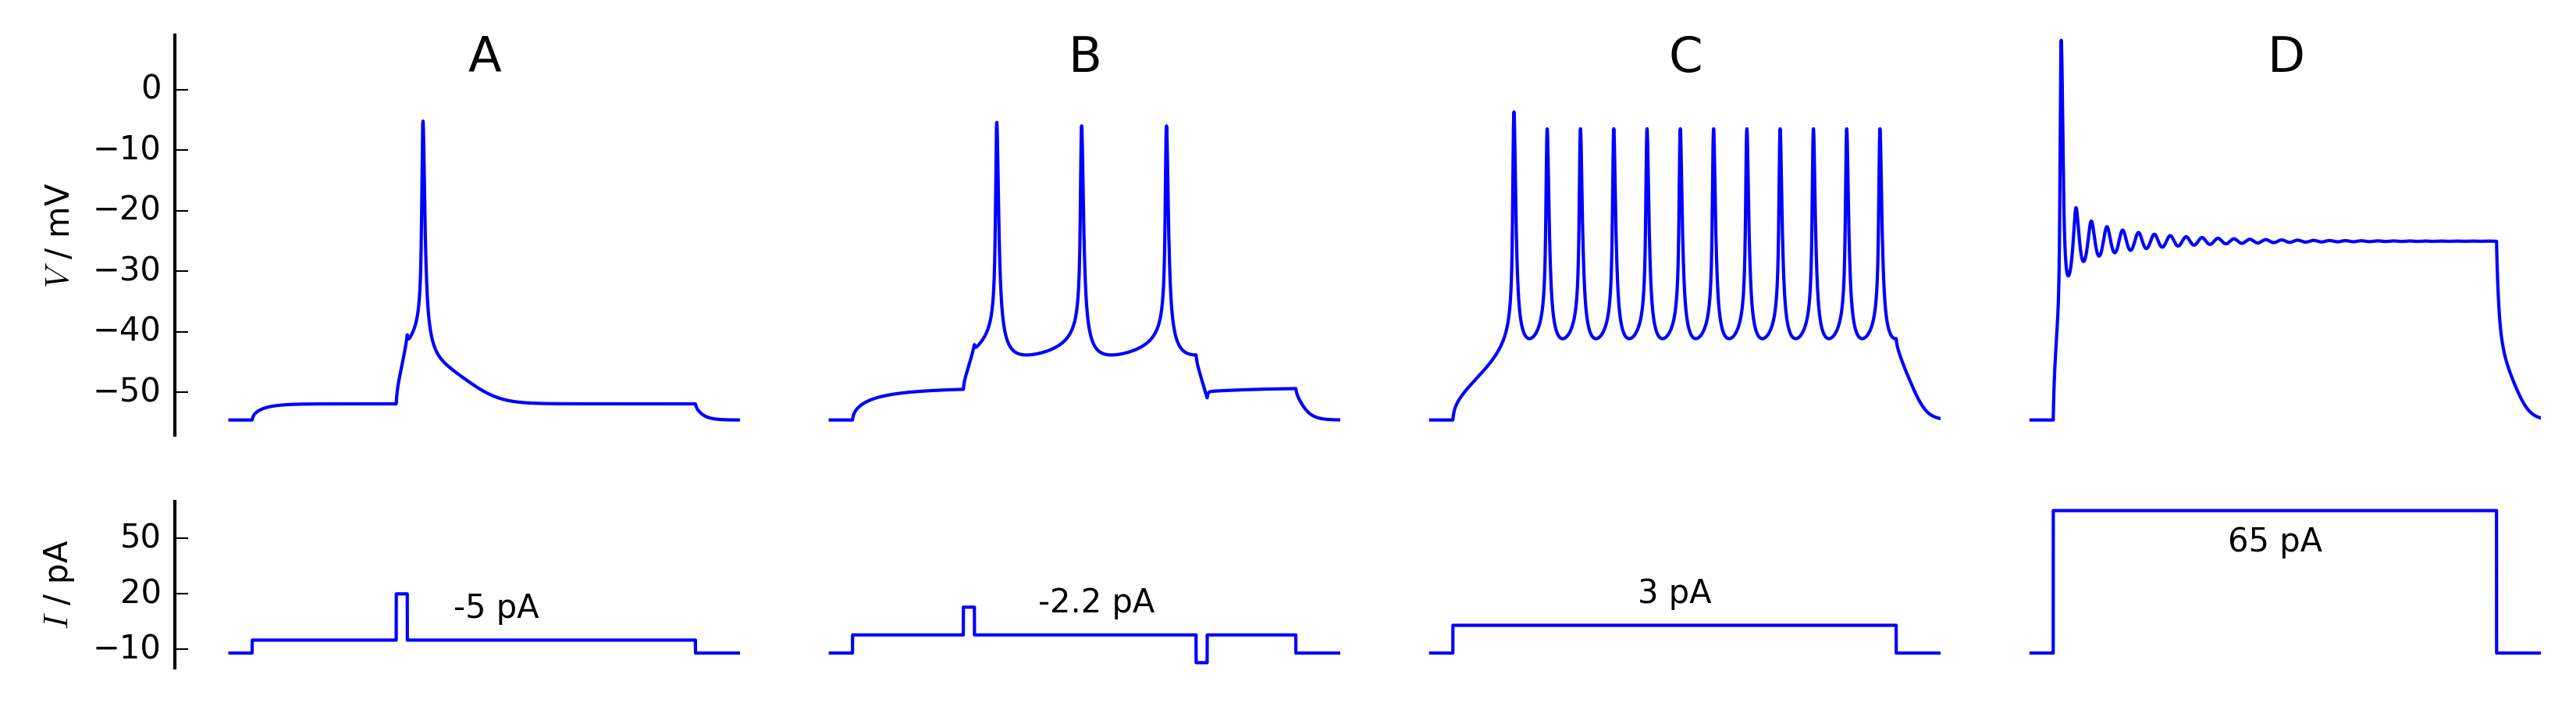
\includegraphics[]{images/voltage_traces.png}
\caption[Membrane potential for different current stimuli
]{Membrane potential (top) for different current stimuli
(bottom). A-D show qualitatively different behaviours according to
table~\ref{regions}. Model at rest ($I$ = -12 pA) initially. Constant
current steps for 200 ms. In A and B, short square current pulses were
added. \textbf{A:} Silent behaviour at low currents. In response to a
short square current pulse, the neuron fires a single spike. \textbf{B:}
Bistable behaviour. The system can be switched from silent to spiking
behaviour (and back) via short square current pulses. \textbf{C:} Tonic
spiking. \textbf{D:} Silent behaviour and oscillations at high
currents.}\label{voltage-traces}
\end{figure}

The model showed four qualitatively different types of behaviour. These
occurred in different regions of the stimulating current $I$, hereafter
denoted as A to D. Table~\ref{regions} shows the values of $I$ for each
region and the associated behaviour. Typical voltage traces for all
regions are depicted in fig.~\ref{voltage-traces}.

For weak stimuli (A), the neuron stayed silent. When the current step
was applied, its membrane potential increased slowly and saturated
towards a new equilibrium value. Subthreshold oscillations were not
observed. In response to a short square current pulse, the neuron fired
a single spike and returned to rest (fig.~\ref{voltage-traces}A). At the
default bias current of $I$ = -12 pA, the neuron had a resting potential
of (-54.56 $\pm$ 0.01) mV.

In region B, the neuron was bistable, i. e. it was able to show both
silent and (tonic) spiking behaviour. Which behaviour was observed
depended on the previous state of the system (hysteresis behaviour,
see~\ref{firing-rate}). The model could be switched from silent to
spiking behaviour by short depolarizing current pulses, or from spiking
to silent behaviour via short hyperpolarizing current pulses
(fig.~\ref{voltage-traces}B). The bistable region was very small
(\textless{} 1 pA, compare table~\ref{regions}).

For higher currents (C), the neuron transitioned to tonic spiking.
Single spikes could not be observed in response to constant current
steps. The rheobase (minimum amount of sustained current input to
stimulate spiking) was (-1.90 $\pm$ 0.01) pA (for simulations of max.
5000 ms). Region C spanned a large range of currents, and spiking
properties differed accordingly. In short, at higher currents the neuron
started to fire earlier, more frequently and with lower spike
amplitudes. A detailed analysis of these properties is given
in~\ref{firing-rate}, \ref{delays} and~\ref{amplitudes}.

For very large stimuli (D), the model stopped firing and became silent
again. In response to the current step, a single spike was emitted.
Subsequently, the membrane potential oscillated towards a stable
equilibrium value (which was much higher than the equilibrium values in
region A).

\begin{table}
\centering
\begin{tabular}{ccc}
\toprule\addlinespace
Region & $I$ / pA & Behaviour\tabularnewline
\midrule
A & ≤ -2.73 & silent\tabularnewline
B & -2.72 to -1.89 & bistable\tabularnewline
C & -1.90 to 59.69 & spiking\tabularnewline
D & ≥ 59.70 & silent (with oscillations)\tabularnewline
\bottomrule
\end{tabular}
\caption[Current regions A to D]{Current regions A to D in which the neuron model showed
qualitatively different behaviours.}\label{regions}
\end{table}

\subsection{Firing Rate}\label{firing-rate}

\begin{figure}
\centering
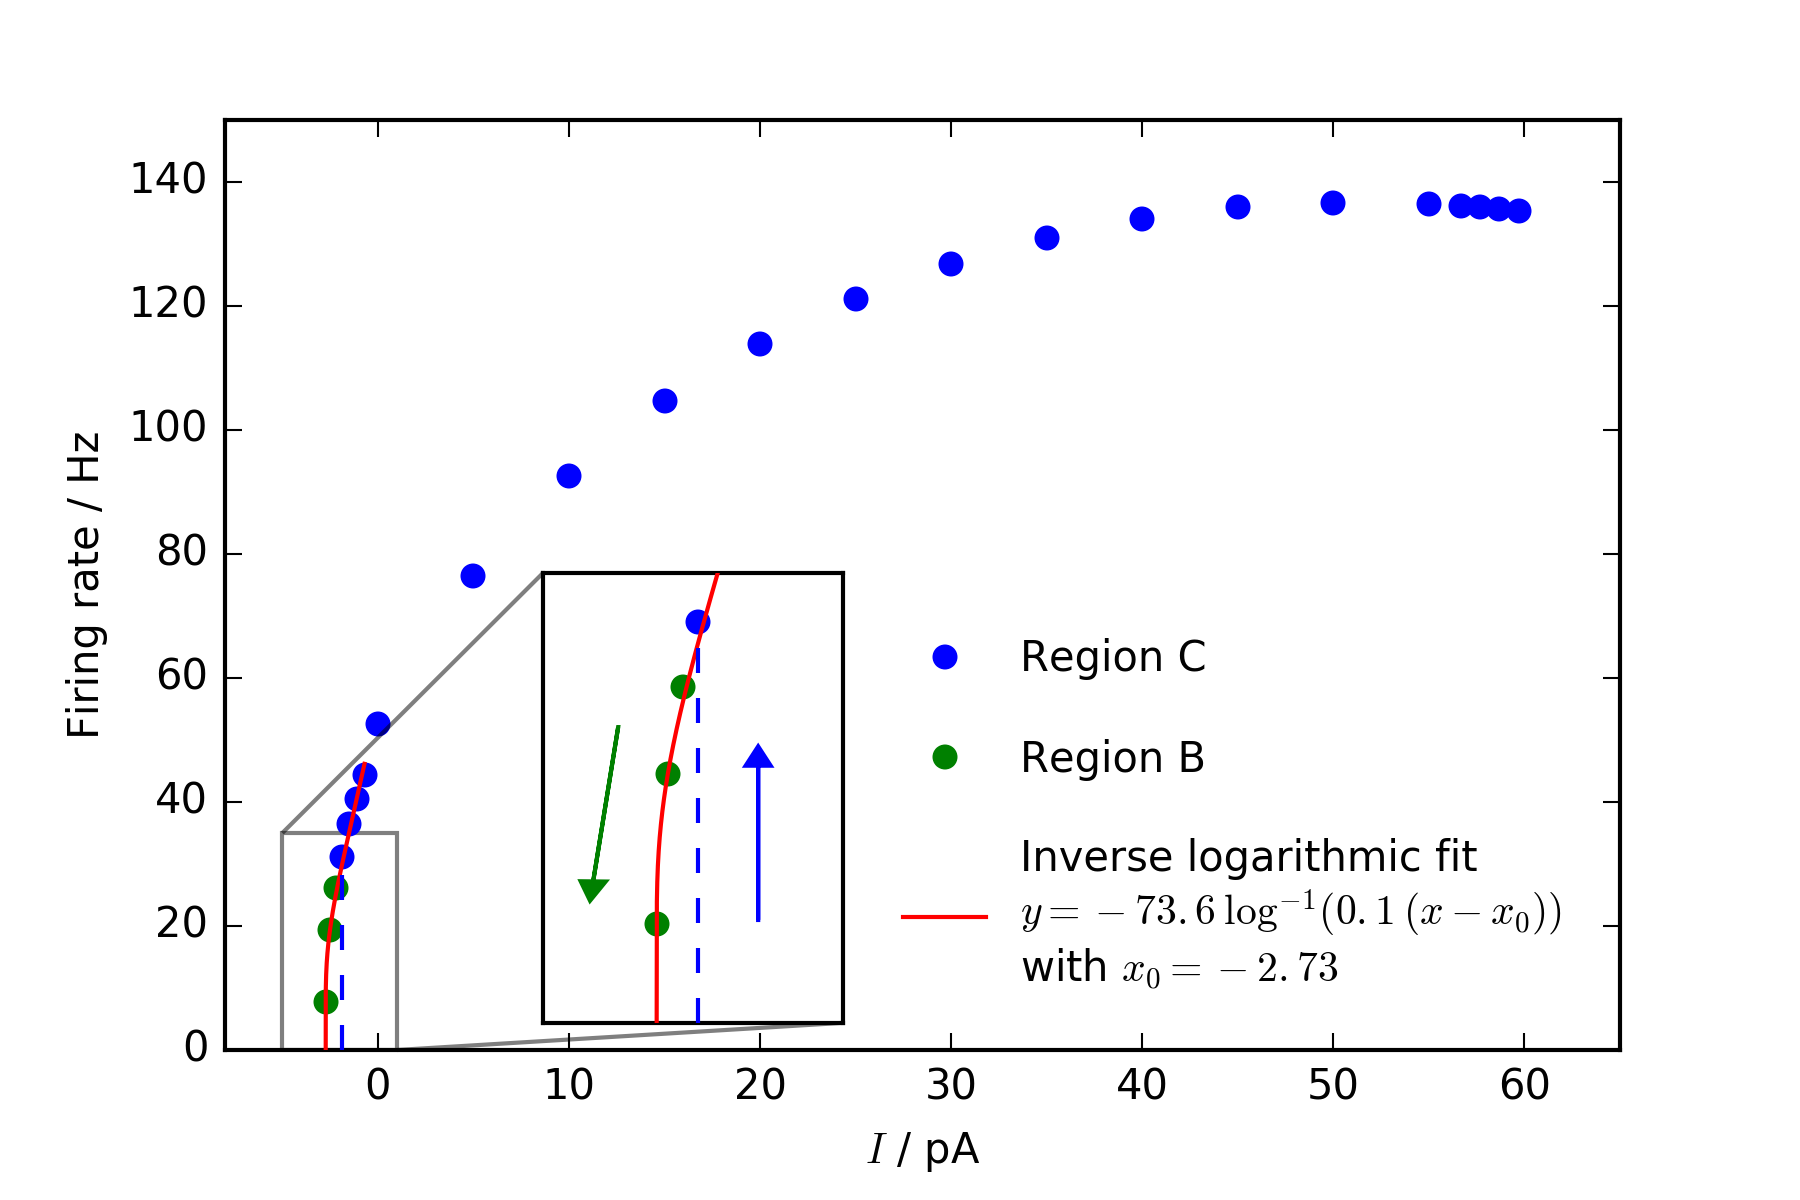
\includegraphics[]{images/f-I-curve.png}
\caption[Firing rate for various current steps (f-I-curve)]{Firing rate for various current steps (f-I-curve). Tonic
spiking in the bistable region B was achieved by decreasing the current
from region C. Arrows indicate hysteresis behaviour. Error bars not
shown due to small size.}\label{f-i-curve}
\end{figure}

For tonic spiking in region B and C, the firing rate of the neuron model
(i. e. the frequency of spikes) was calculated from simulations. It is
shown in the so called f-I-curve in fig.~\ref{f-i-curve}. The firing
rate increased with the strength of the stimulation and approached a
constant value for high current stimuli. In all simulations, spiking was
very regular, i. e. the period between subsequent spikes was more or
less constant. Adaptation or bursting was not observed.

At the onset of spiking, the neuron showed a clear hysteresis behaviour:
If the current was slowly increased (starting with silent behaviour in
region A), the neuron stayed silent in the bistable region B. At the
transition to region C (rheobase), it started to spike tonically with
non-zero frequencies (blue arrow in fig.~\ref{f-i-curve}). Conversely,
if the current was slowly decreased (starting with spiking behaviour in
region C), the neuron continued to spike in the bistable region B. Its
firing rate approached zero at the transition to the silent region A
(red arrow in fig.~\ref{f-i-curve}). According to the (extended) Hodgkin
classification of excitability (see~\ref{excitability}), the neuron is
therefore class 2 excitable and class 1 spiking. This indicates that the
silence-tonic and tonic-silence transitions are governed by different
bifurcations.

For small current stimuli (near the onset of spiking), an inverse
logarithmic function could be fit to the firing rate (red curve in
fig.~\ref{f-i-curve}). According to the scaling laws referenced
in~\ref{excitability}, this implies that the bifurcation at the
transition from region A to B is a homoclinic bifurcation.

\subsection{Delays}\label{delays}

In region C (tonic spiking), the neuron needed some time to start
spiking after the current step was applied (see voltage trace in
fig.~\ref{voltage-traces}C). This delay to first spike was calculated
from simulations and is shown in fig.~\ref{plot-delays}. The delay was
negligible for large currents, but increased notably for small currents
close to the onset of spiking. By tweaking the decimal numbers of the
stimulating current (and therefore getting it closer to the exact
rheobase current), the delay could be increased to arbitrarily large
values (for example 2.7 s at an amplitude of 1.90 pA).

\begin{figure}
\centering
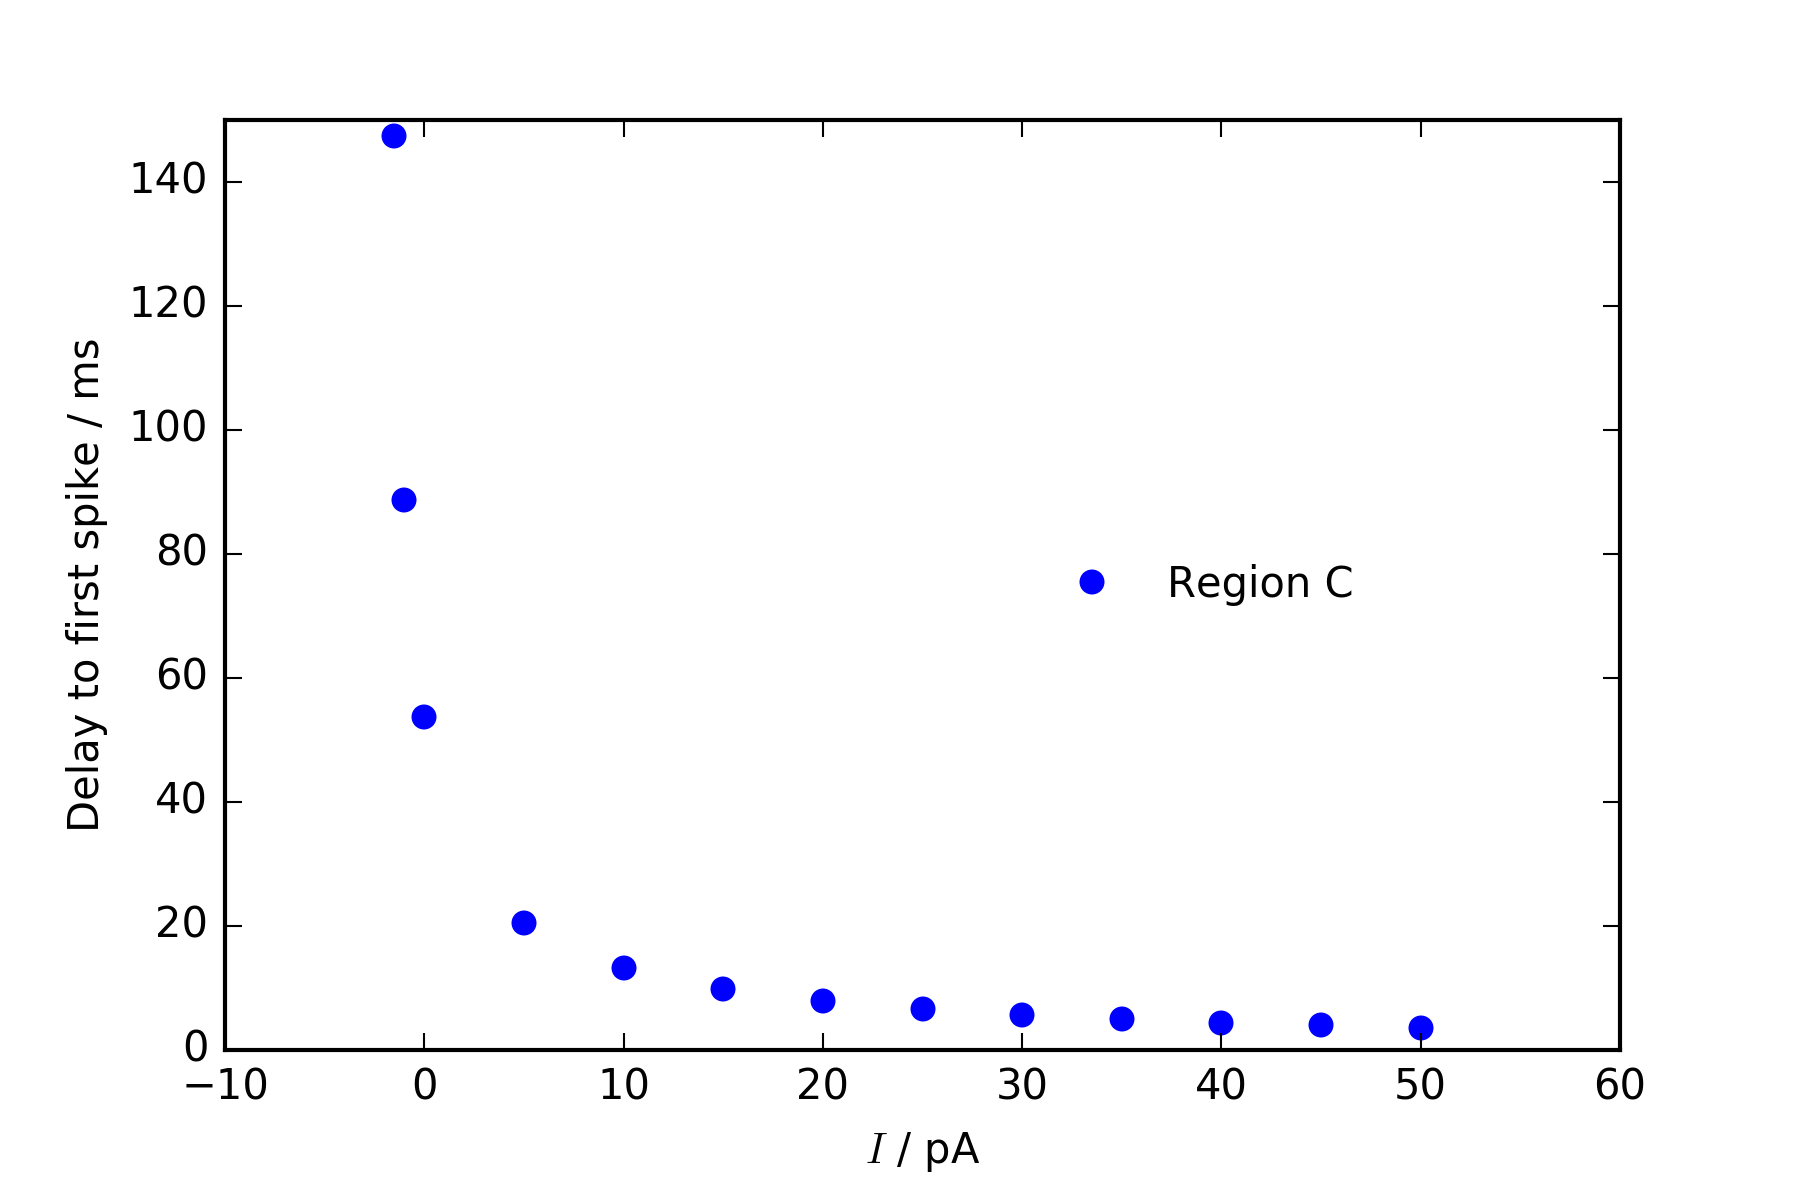
\includegraphics[]{images/delay.png}
\caption[Delay to first spike for various current steps]{Delay to first spike for various current steps. Model was
at rest initially, then a constant current step was injected and the
time to the first spike measured (spike detection via voltage threshold
of -25 mV). Error bars not shown due to small size.}\label{plot-delays}
\end{figure}

\subsection{Spike Amplitudes}\label{amplitudes}

For tonic spiking (B and C), the spike minima and maxima were calculated
(minimum means the minimal membrane potential between spikes, maximum
means the maximal membrane potential during a spike). Spike amplitudes
were calculated as the difference between minima and maxima.
Fig.~\ref{minima-maxima-amplitudes} presents all values for different
current steps.

Spike amplitudes were large for strong stimuli and vanished for weak
stimuli. At the transition to region D, they could be approximated by a
square function (red curve in fig.~\ref{minima-maxima-amplitudes}).
This implies that there is a supercritical Hopf bifurcation at this
transition (see~\ref{excitability}).

\begin{figure}
\centering
\captionsetup[subfigure]{labelformat=empty}
\subfloat[]{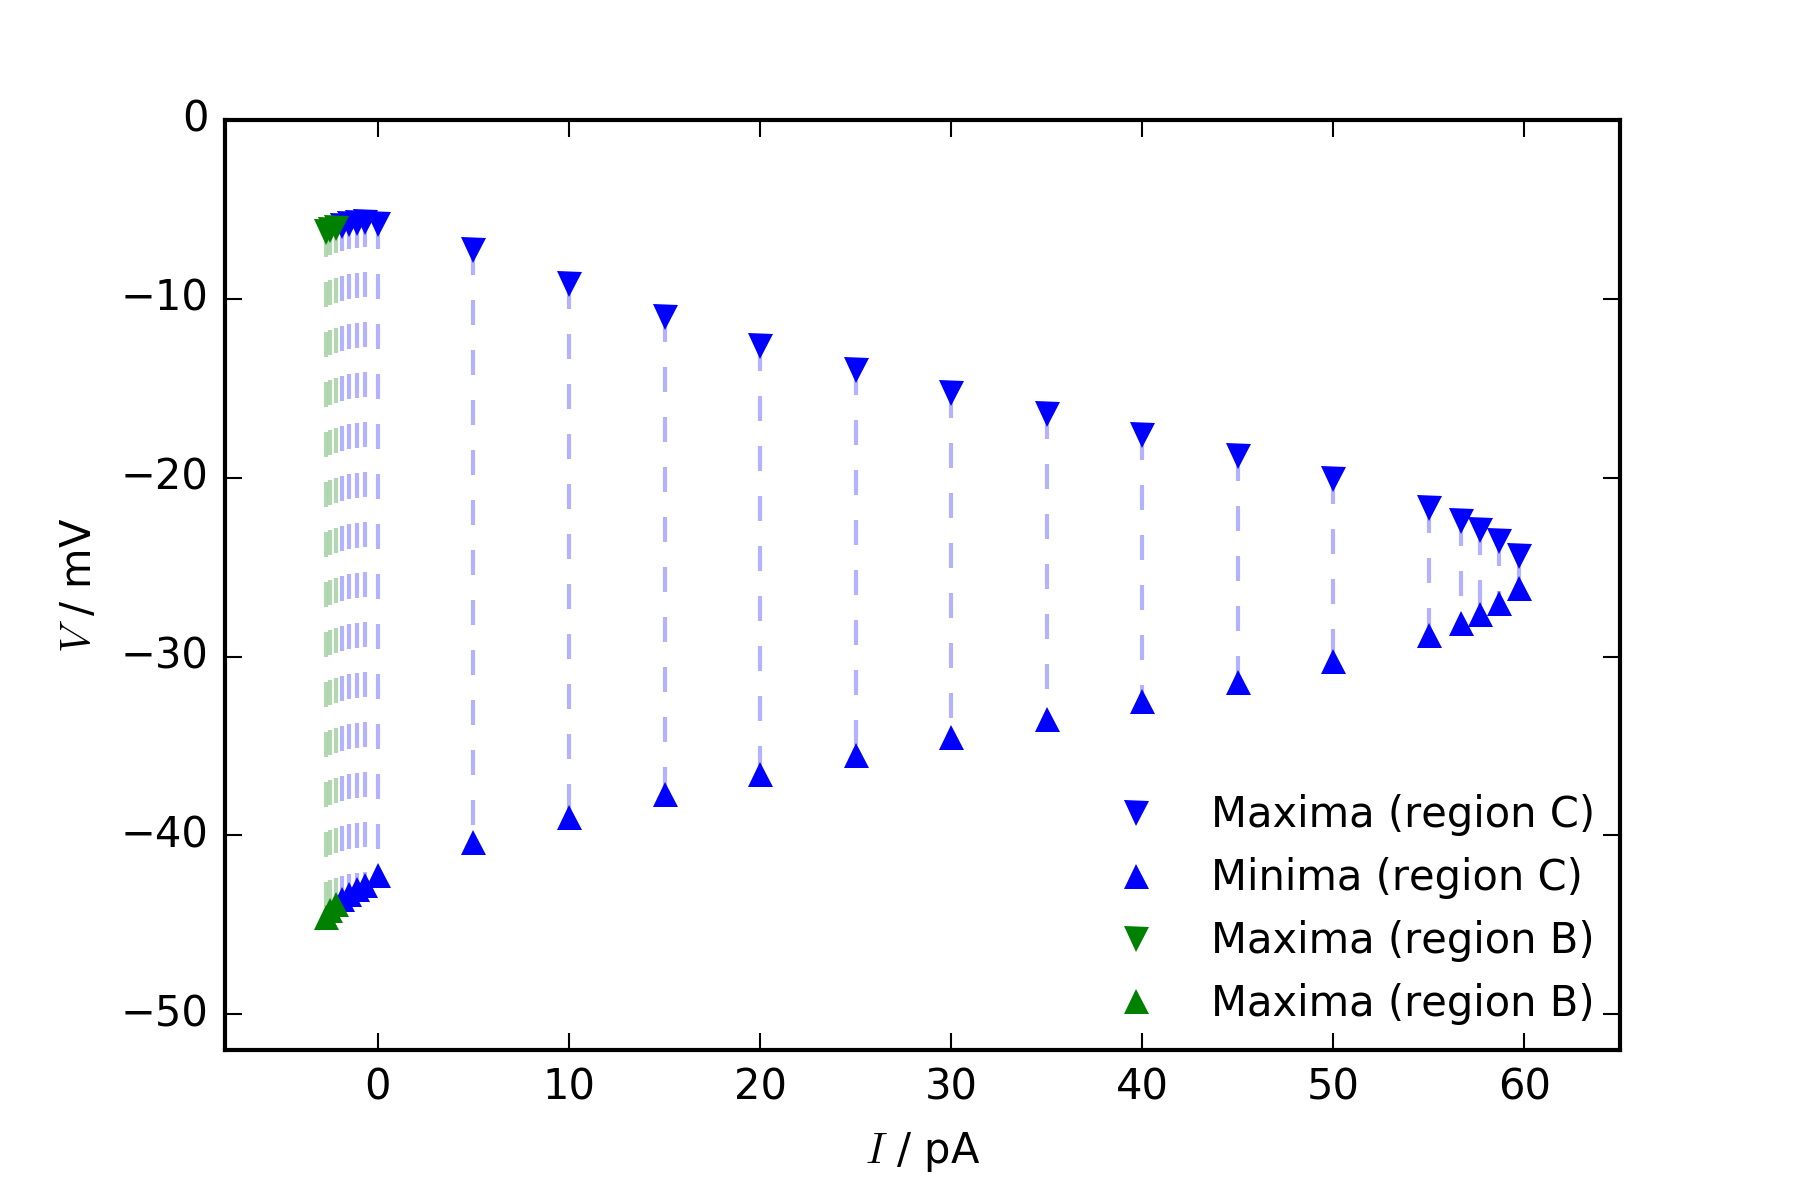
\includegraphics[]{images/min_max.png}}
\\
\subfloat[]{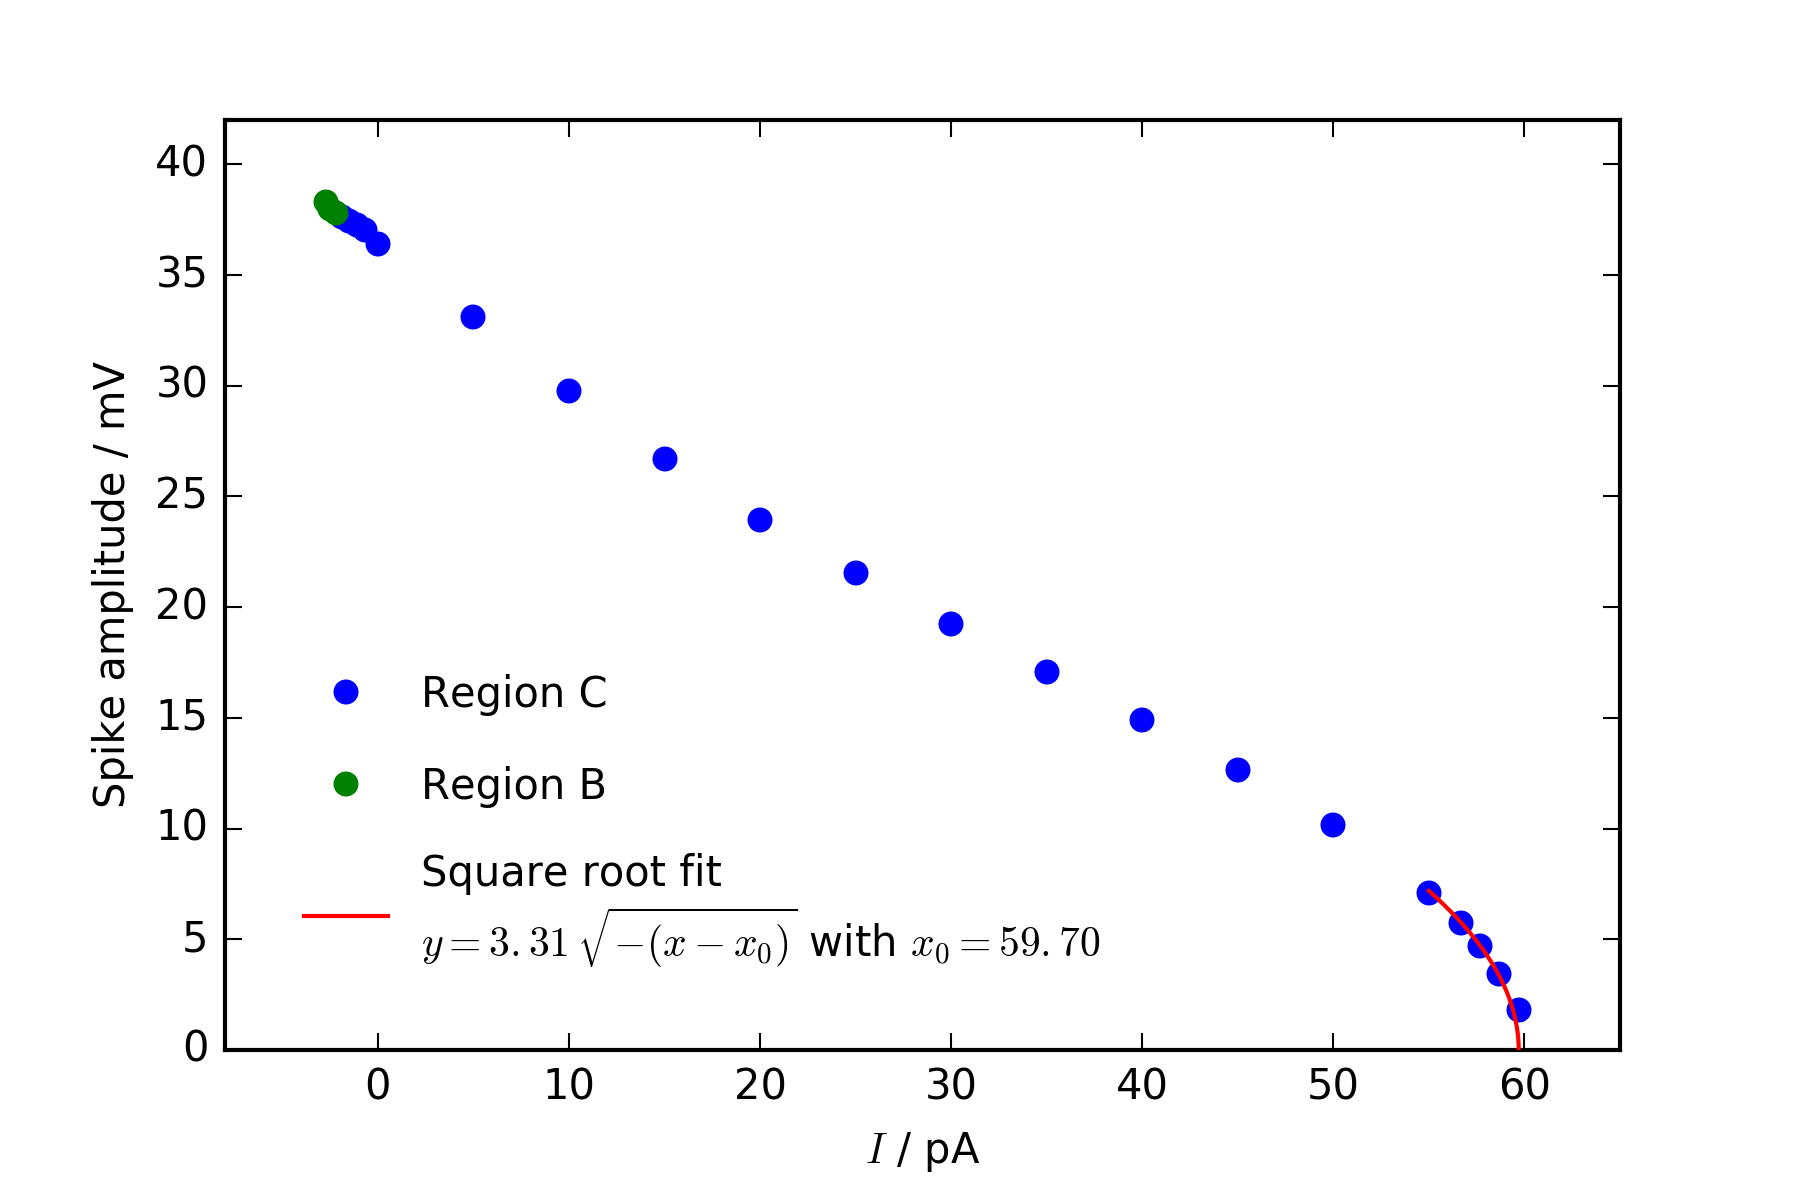
\includegraphics[]{images/amplitudes.png}}
\caption[Spike minima, maxima and amplitudes for
various current steps]{Spike minima, maxima (top) and amplitudes (bottom) for
various current steps. Dashed lines indicate amplitudes. Setup equal
to fig.~\ref{f-i-curve}. Error bars not shown due to small
size.}\label{minima-maxima-amplitudes}
\end{figure}

\section{Steady-State I-V-Curve}\label{i-v-results}

As an intermediate step to the bifurcation analysis, the steady-state
I-V-curve of the model was calculated (see~\ref{i-v-methods}). This
curve shows the overall current $I_{\infty}$ that is flowing into the
neuron at a given membrane potential $V$, if the gating variables have
settled into steady state. Fig.~\ref{i-v-curve} depicts the curve for
four representative values of the stimulating current $I$.

\begin{figure}
\centering
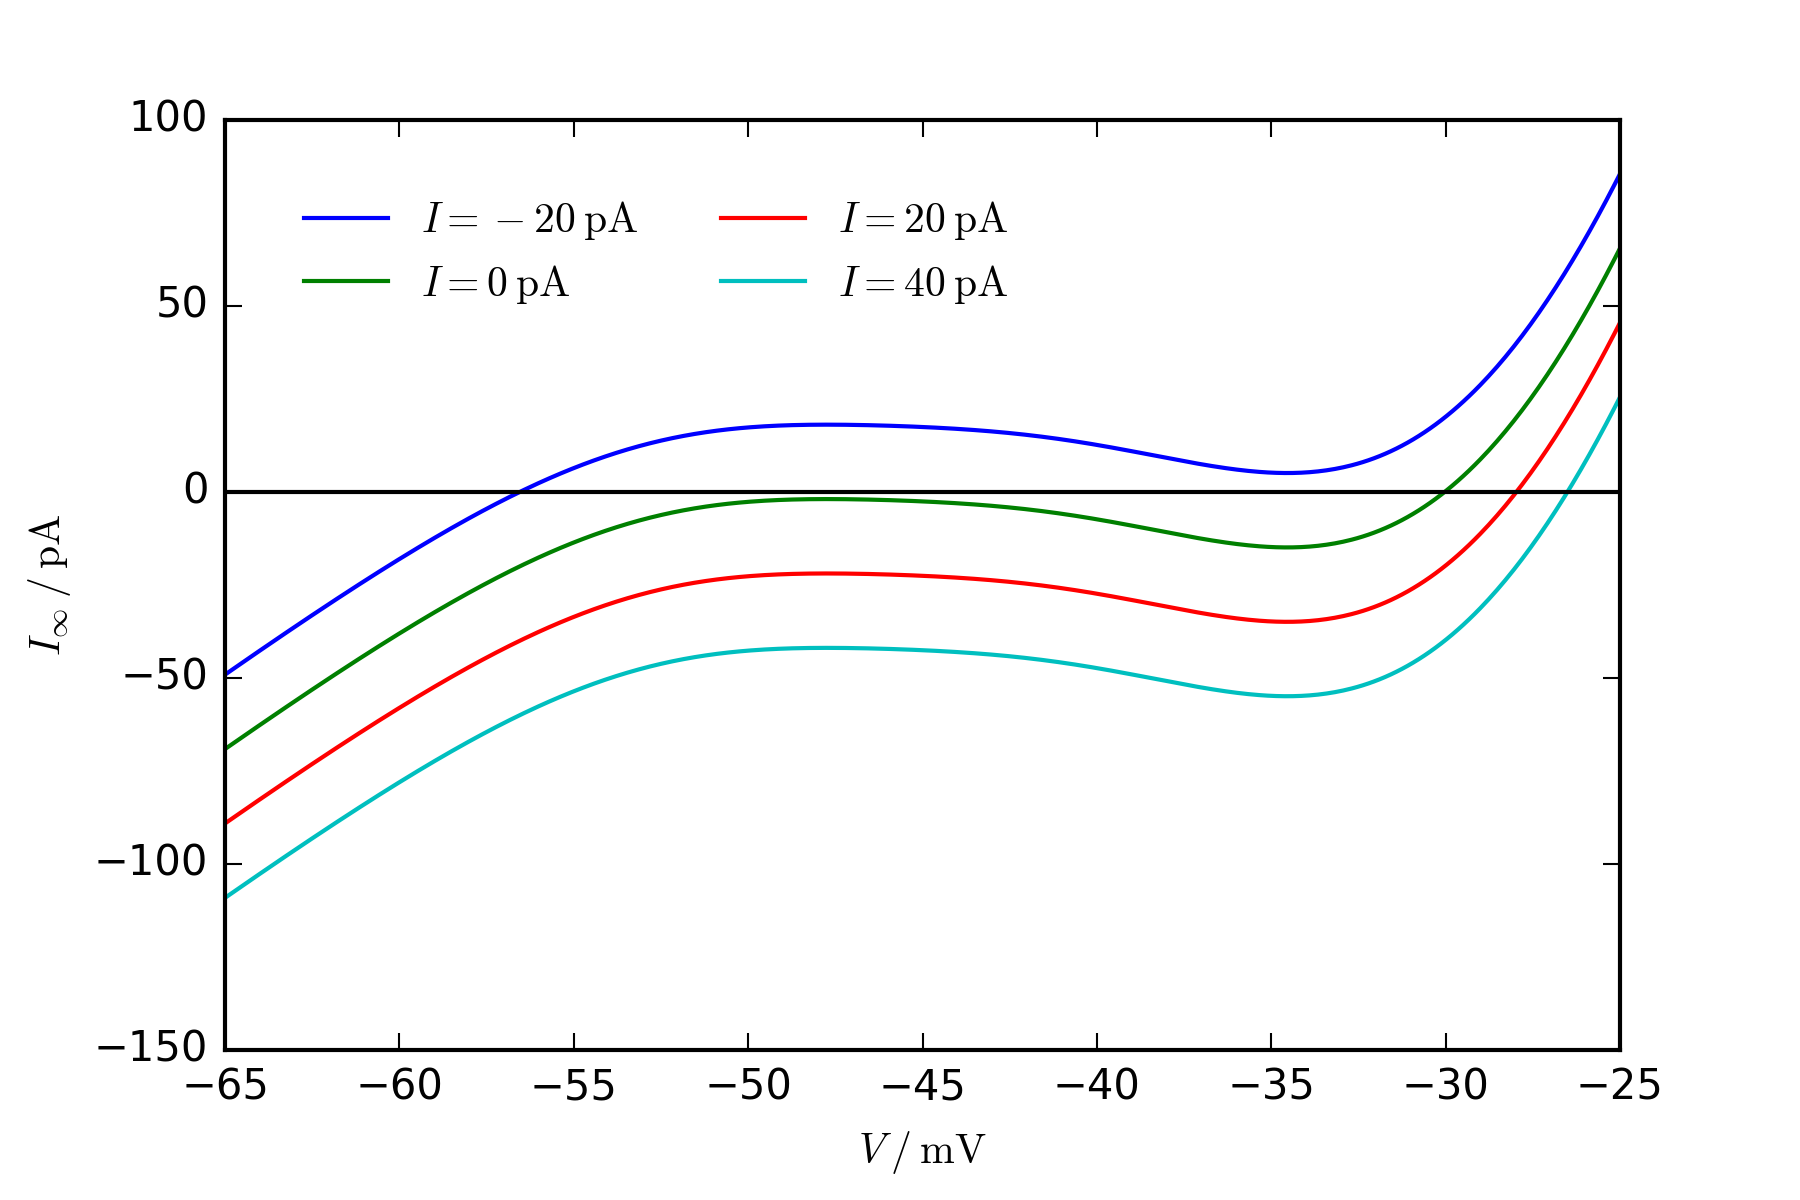
\includegraphics[]{images/I-V-curve.png}
\caption[Steady-state I-V-curve for different values of the
stimulating current $I$]{Steady-state I-V-curve for different values of the
stimulating current $I$.}\label{i-v-curve}
\end{figure}

In all cases, the curve had a N-shape. At the intersections with the
horizontal axis, there is no current flowing into or out of the neuron.
Hence, these points represent equilibria of the system (Izhikevich 2007,
p.~161). However, based on the I-V-curve itself no conclusions about
their stability can be drawn.

For weak stimuli (region A), the steady-state I-V-curve showed an
equilibrium at low membrane potentials $V$. As the neuron is silent in
this region (fig.~\ref{voltage-traces}A), the equilibrium is probably
stable. As $I$ was increased, the curve moved downwards (i. e. to
smaller values of $I_{\infty}$). Subsequently, the right arc of the
curve crossed the horizontal axis and created two new equilibria. At $I$
= -2.72 pA (transition from region A to B), no qualitative change in the
I-V-curve could be observed. At $I$ = -1.90 pA (transition from region B
to C), the left arc of the curve crossed the horizontal axis. Hence, two
intersections with the horizontal axis (i. e. equilibria) merged and
disappeared. This indicates a saddle-node bifurcation at the onset of
spiking. After the bifurcation (in region C), the I-V-curve had only one
equilibrium left. As the neuron was spiking repeatedly in this region,
the equilibrium is probably unstable. At $I$ = 59.70 pA (transition from
region C to D), the I-V-curve showed no qualitative change. However, the
monotonicity of the curve at this transition indicates a Hopf
bifurcation (Izhikevich 2007, p.~161).

\section{Bifurcation Analysis}\label{bifurcation-analysis}

The neuron model of MN1-Ib represents a dynamical system with eight
dimensions. The state variables are the membrane potential $V$ and the
gating variables $m_{Ks}$, $m_{Kf}$, $h_{Kf}$, $h_{Kf2}$, $m_{Na}$,
$h_{Na}$, $m_{NaP}$. Therefore, the Jacobian (see~\ref{equilibria}) has
eight eigenvalues.

Equilibria and limit cycles of the system were analysed via numerical
continuation (see~\ref{numerical-continuation}). Several bifurcations of
codimension 1 were detected in response to changes of the stimulating
current $I$. These bifurcations alter the qualitative behaviour of the
neuron, and correspond to the transitions between regions A to D
described in~\ref{qualitative-behaviour}. The bifurcation diagram in
fig.~\ref{bifurcation-diagram} shows the location of equilibria, limit
cycles and bifurcations.

To give a better impression of the phase space, some exemplary
situations from regions A to D are shown in
fig.~\ref{phase-space-plots}. These plots depict two of the eight
dimensions of the phase space, namely the membrane potential $V$ and the
activation of the fast potassium current $m_{Kf}$. As in most neuron
models, the dynamics in the MN1-Ib model can be divided into one fast
and one slow subprocess (Izhikevich 2007, pp.~147-150). Here, $V$
belongs to the fast, $m_{Kf}$ to the slow subprocess. Therefore,
plotting these variables against each other yields a good impression of
the actual phase portrait. The trajectories in the plots correspond to
the voltage traces in fig.~\ref{voltage-traces}.

\begin{figure}
\centering
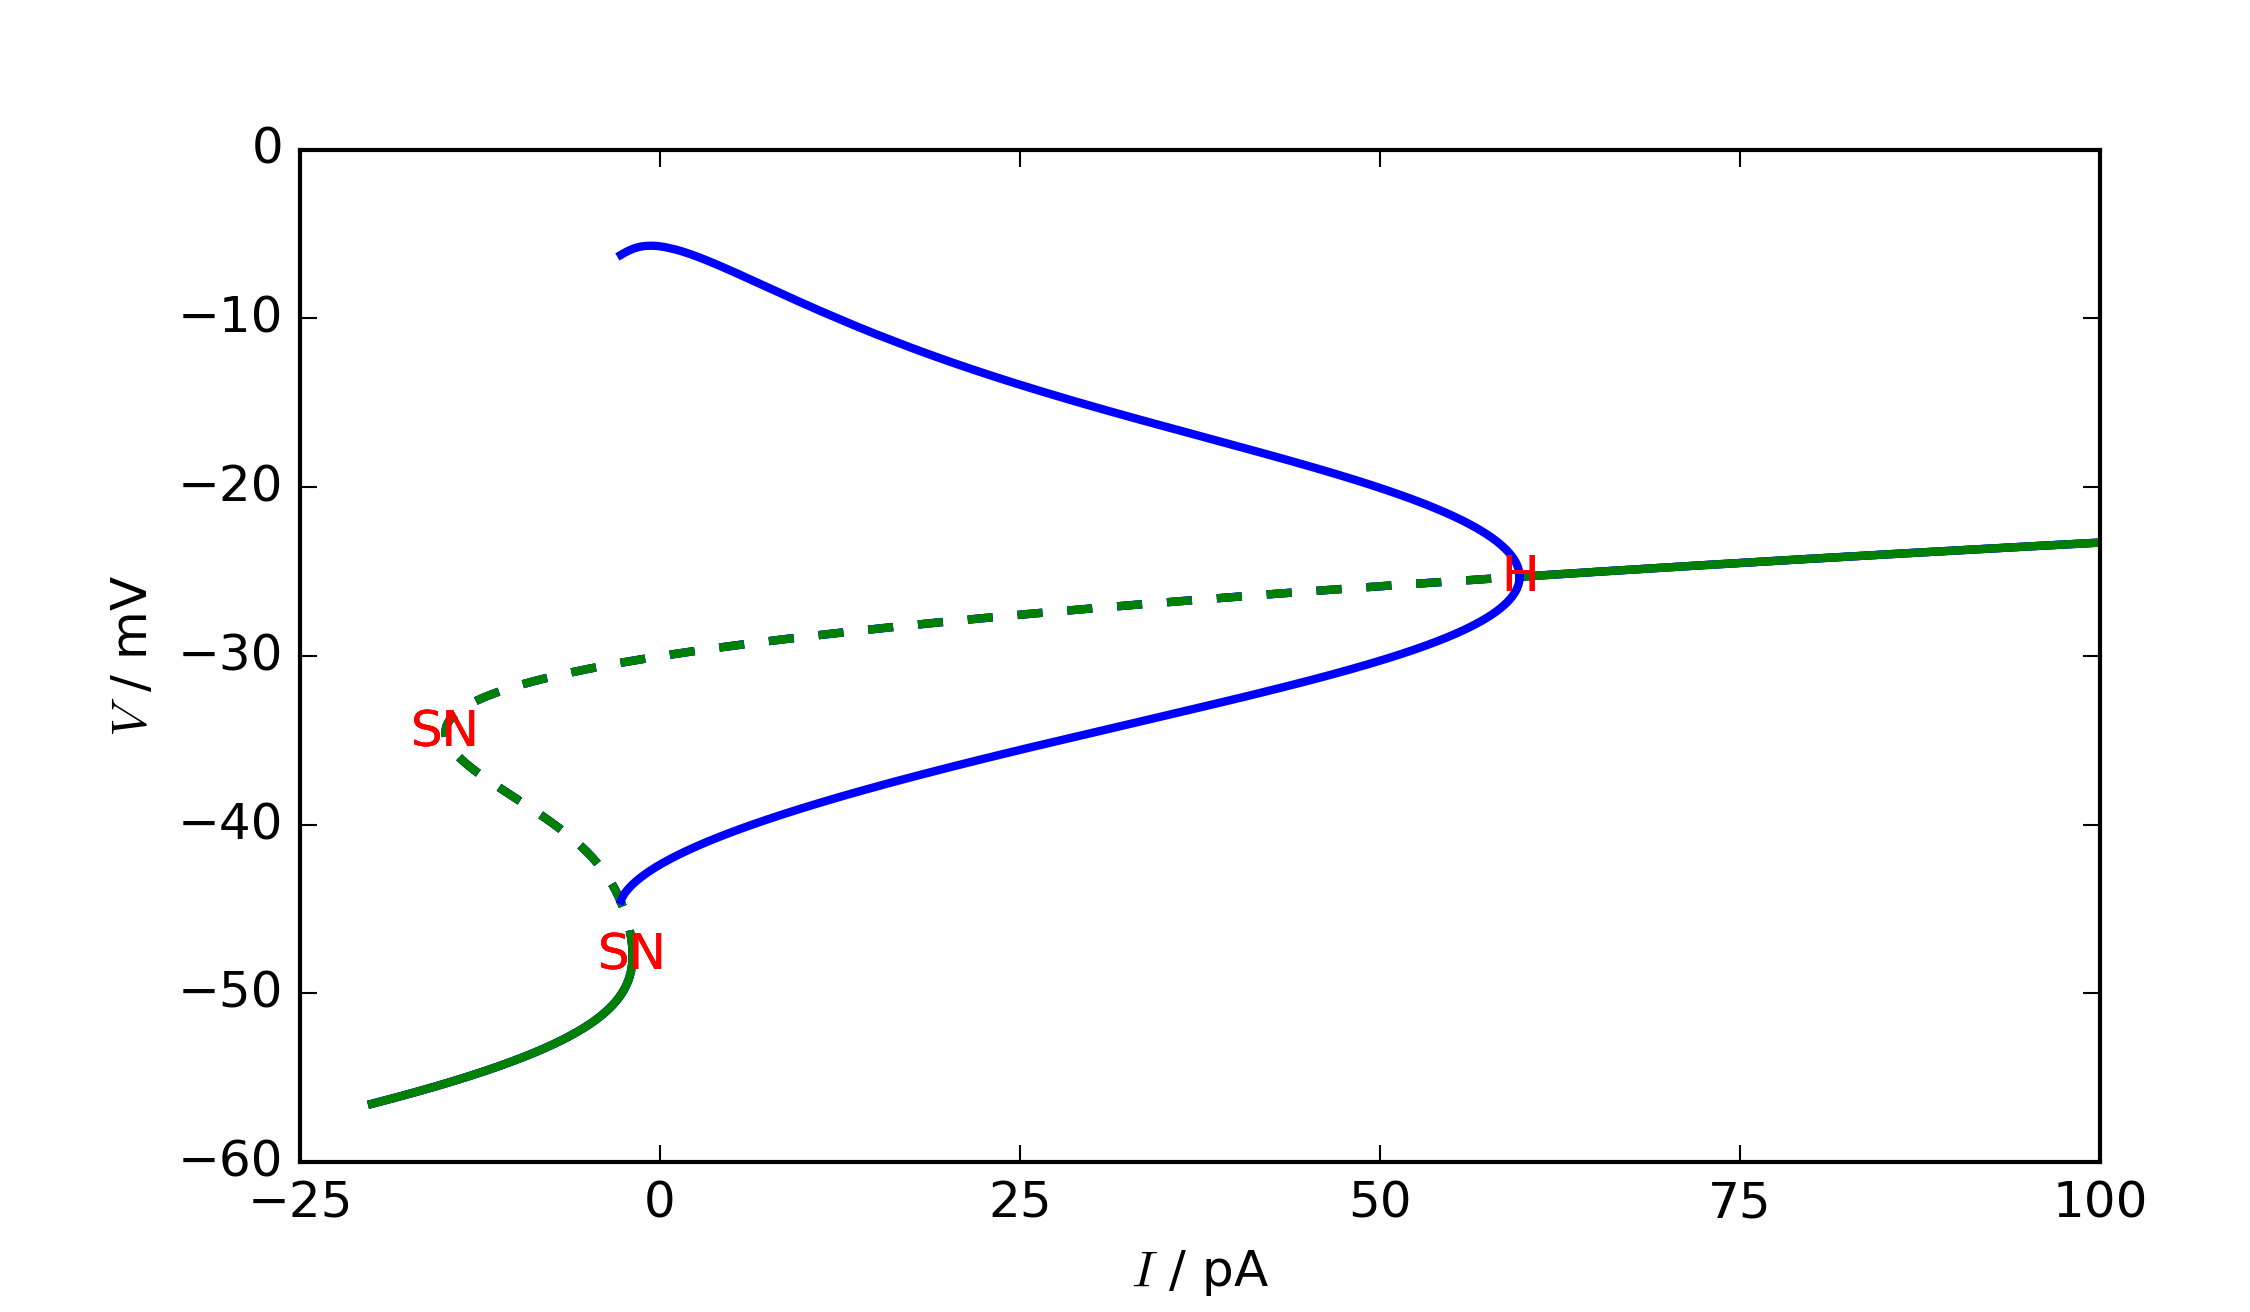
\includegraphics[]{images/bifurcation.png}
\caption[Bifurcation diagram for changing $I$]{Bifurcation diagram for changing $I$. Green solid line:
Stable equilibrium. Green dashed line: Unstable equilibrium. Blue line:
Minimum/maximum of limit cycle. SN: Saddle-node bifurcation. H: Hopf
bifurcation.}\label{bifurcation-diagram}
\end{figure}

\begin{figure}
\centering
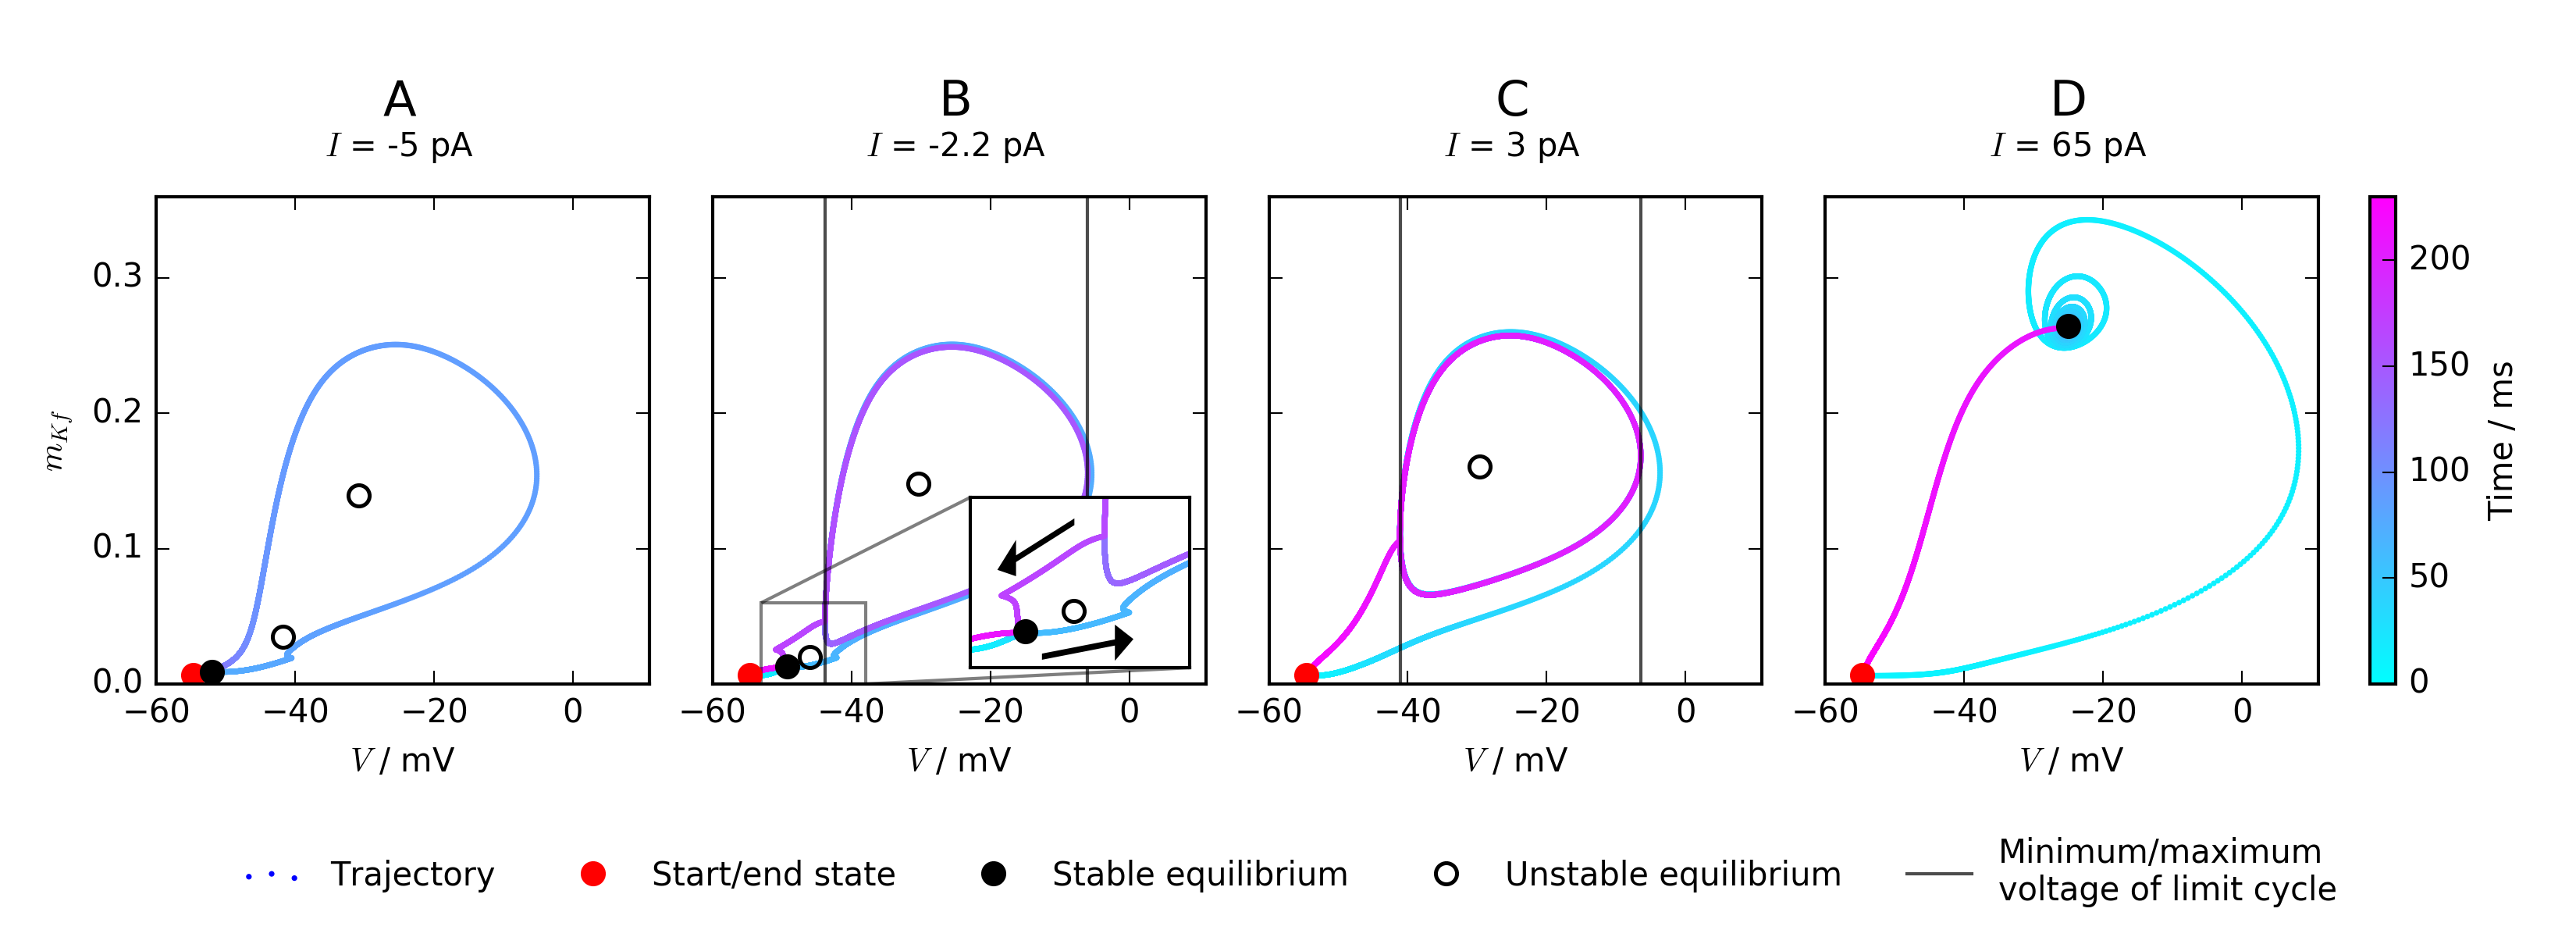
\includegraphics[]{images/phase_space.png}
\caption[Two-dimensional subset of the phase space for different
stimulating currents $I$]{Two-dimensional subset of the phase space for different
stimulating currents $I$. Trajectories correspond to voltage traces
in fig.~\ref{voltage-traces}. Locations of equilibria and the limit
cycle were taken from the bifurcation diagram in
fig.~\ref{bifurcation-diagram}.}\label{phase-space-plots}
\end{figure}

\subsection{Overview}\label{overview}

For low values of $I$, the system had a stable equilibrium (solid blue
line in fig.~\ref{bifurcation-diagram}, black circle in
fig.~\ref{phase-space-plots}A). This corresponds to the silent behaviour
observed in region A (see~\ref{qualitative-behaviour}). As the
stimulating current was increased, the stable equilibrium moved slowly
towards higher values of the membrane potential $V$. Two unstable
equilibria originated from a saddle-node bifurcation (SN in
fig.~\ref{bifurcation-diagram}, compare also the right arc in the
I-V-curve,~\ref{i-v-results}). However, these unstable equilibria did
not alter the (silent) behaviour of the model at this point.

At $I$ = -2.72 pA (transition from region A to B), a stable limit cycle
was created via homoclinic bifurcation. In
fig.~\ref{bifurcation-diagram} and fig.~\ref{phase-space-plots}B and C,
the limit cycle is indicated by its minimal and maximal membrane
potential. At $I$ = -1.90 pA (transition from region B to C), a
saddle-node bifurcation extinguished the stable equilibrium. This is in
agreement with the class 2 excitability of the neuron observed in
simulations (see~\ref{firing-rate}) and the results from the
steady-state I-V-curve (see~\ref{i-v-results}).

With increasing $I$, the amplitude of the limit cycle decreased. At $I$
= 59.70 pA (transition from region C to D), it became so small that it
merged with the unstable equilibrium inside of it via a supercritical
Hopf bifurcation (H in fig.~\ref{bifurcation-diagram}). This created a
new stable equilibrium, which governed the silent behaviour in region D.

\subsection{Onset of spiking}\label{onset-of-spiking}

The transition from silent to spiking behaviour is controlled by the
interplay of two bifurcations: The homoclinic bifurcation at $I$ = -2.72
pA creates the stable limit cycle, which corresponds to tonic spiking.
The saddle-node bifurcation at $I$ = -1.90 pA extinguishes the stable
equilibrium, which corresponds to silent behaviour.

Between these bifurcations (i. e. in region B), the stable equilibrium
and the stable limit cycle coexist. The trajectory of the system can
stay on either one. This explains the bistability of silence and tonic
spiking described in~\ref{qualitative-behaviour} and~\ref{firing-rate}.
In simulations, short square current pulses could be used to switch the
neuron between these two behaviours (fig.~\ref{voltage-traces}B). The
phase portrait explains this effect (fig.~\ref{phase-space-plots}B):
Between the stable equilibrium and the stable limit cycle, there is an
unstable equilibrium. Its stable manifold serves as a separatrix: All
trajectories on the left move towards the stable equilibrium, all
trajectories on the right move towards the limit cycle. The current
pulses ``push'' the trajectory across this separatrix (and thus towards
the equilibrium or the limit cycle), as indicated by the arrows in the
inset in fig.~\ref{phase-space-plots}B.

At the onset of spiking, the neuron showed a considerable delay to first
spike in simulations (see~\ref{delays}). This effect can be explained by
the saddle-node bifurcation: Before the bifurcation, the system has a
stable equilibrium. At its position in phase space, all differential
equations are zero. After the bifurcation, this equilibrium is gone, but
the differential equations at its former position are still very small.
Therefore, the trajectories move very slowly through this region - they
are affected by the ``ghost'' of the equilibrium, which causes the delay
to first spike (Izhikevich 2007, p.~246).

\subsection{Amplitude and Frequency of the Limit
Cycle}\label{amplitude-and-frequency-of-the-limit-cycle}

With increasing $I$, the amplitude of the stable limit cycle became
smaller. The shape of its minimal and maximal membrane potential
(fig.~\ref{bifurcation-diagram}) matches the spike minima and maxima
recorded in simulations (fig.~\ref{minima-maxima-amplitudes}).
In~\ref{amplitudes}, the spike amplitudes near the end of spiking were
fitted by a square-root function. This predicted a supercritical Hopf
bifurcation, which was verified by numerical continuation
(fig.~\ref{bifurcation-diagram}).

During the numerical continuation of the limit cycle, the frequencies of
the cycle were recorded (results not shown). Their values replicated the
f-I-curve in fig.~\ref{f-i-curve}. As described in~\ref{firing-rate},
this curve was fit by an inverse logarithm at the onset of spiking. This
predicted a fold limit cycle bifurcation, which was verified by
numerical continuation (fig.~\ref{bifurcation-diagram}).

\subsection{End of spiking}\label{end-of-spiking}

The transition from spiking to silent behaviour was caused by a
supercritical Hopf bifurcation at $I$ = 59.70 pA. This bifurcation
created a stable equilibrium. Its eigenvalues were analysed from the
output of the numerical continuation. As expected, they contained
imaginary parts and unmasked the equilibrium as a focus. This explains
the oscillations of the neuron in region D (fig.~\ref{voltage-traces}D,
see also oscillations of the trajectory around the equilibrium in
fig.~\ref{phase-space-plots}D).

\section{Behaviour at Different Ion Current
Parameters}\label{two-par-cont}

Numerical continuation in one parameter (the stimulating current $I$)
was able to explain the behavioural repertoire of the neuron. To
investigate how this repertoire changes if we alter the parameters of
the model, numerical continuation in two parameters ($I$ and one other
parameter) was employed. Specifically, the analysis here focuses on the
conductances of the model ($g_{leak}$, $g_{Ks}$, $g_{Kf}$, $g_{Na}$,
$g_{NaP}$). These variables represent the strength of the associated
currents (compare eq.~\ref{currents-hh}): If a conductance is zero,
there is no current at all; if the conductance is high, the current is
strong. Thus, analysing the conductances can yield insight about the
role of each ion current for model behaviour.

Fig.~\ref{two-par-cont-plots} presents the results of the two-parameter
continuation. Each diagram shows how the locations of the codimension-1
bifurcations (i. e. at which value of $I$ they occur) change, if one
conductance is altered (vertical axis). Therefore, a ``horizontal
slice'' of the plot at one specific conductance value corresponds to a
(one-parameter) bifurcation diagram as shown in
fig.~\ref{bifurcation-diagram}. In all diagrams, codimension-2
bifurcations are indicated by letters, default parameter values are
indicated by dashed lines. Most of the effects revealed by two-parameter
continuation were subsequently analysed in more detail, either by
simulation or by plotting one-parameter bifurcation diagrams as in
fig.~\ref{bifurcation-diagram}.

\begin{figure}
\centering
\captionsetup[subfigure]{labelformat=empty}
\subfloat[]{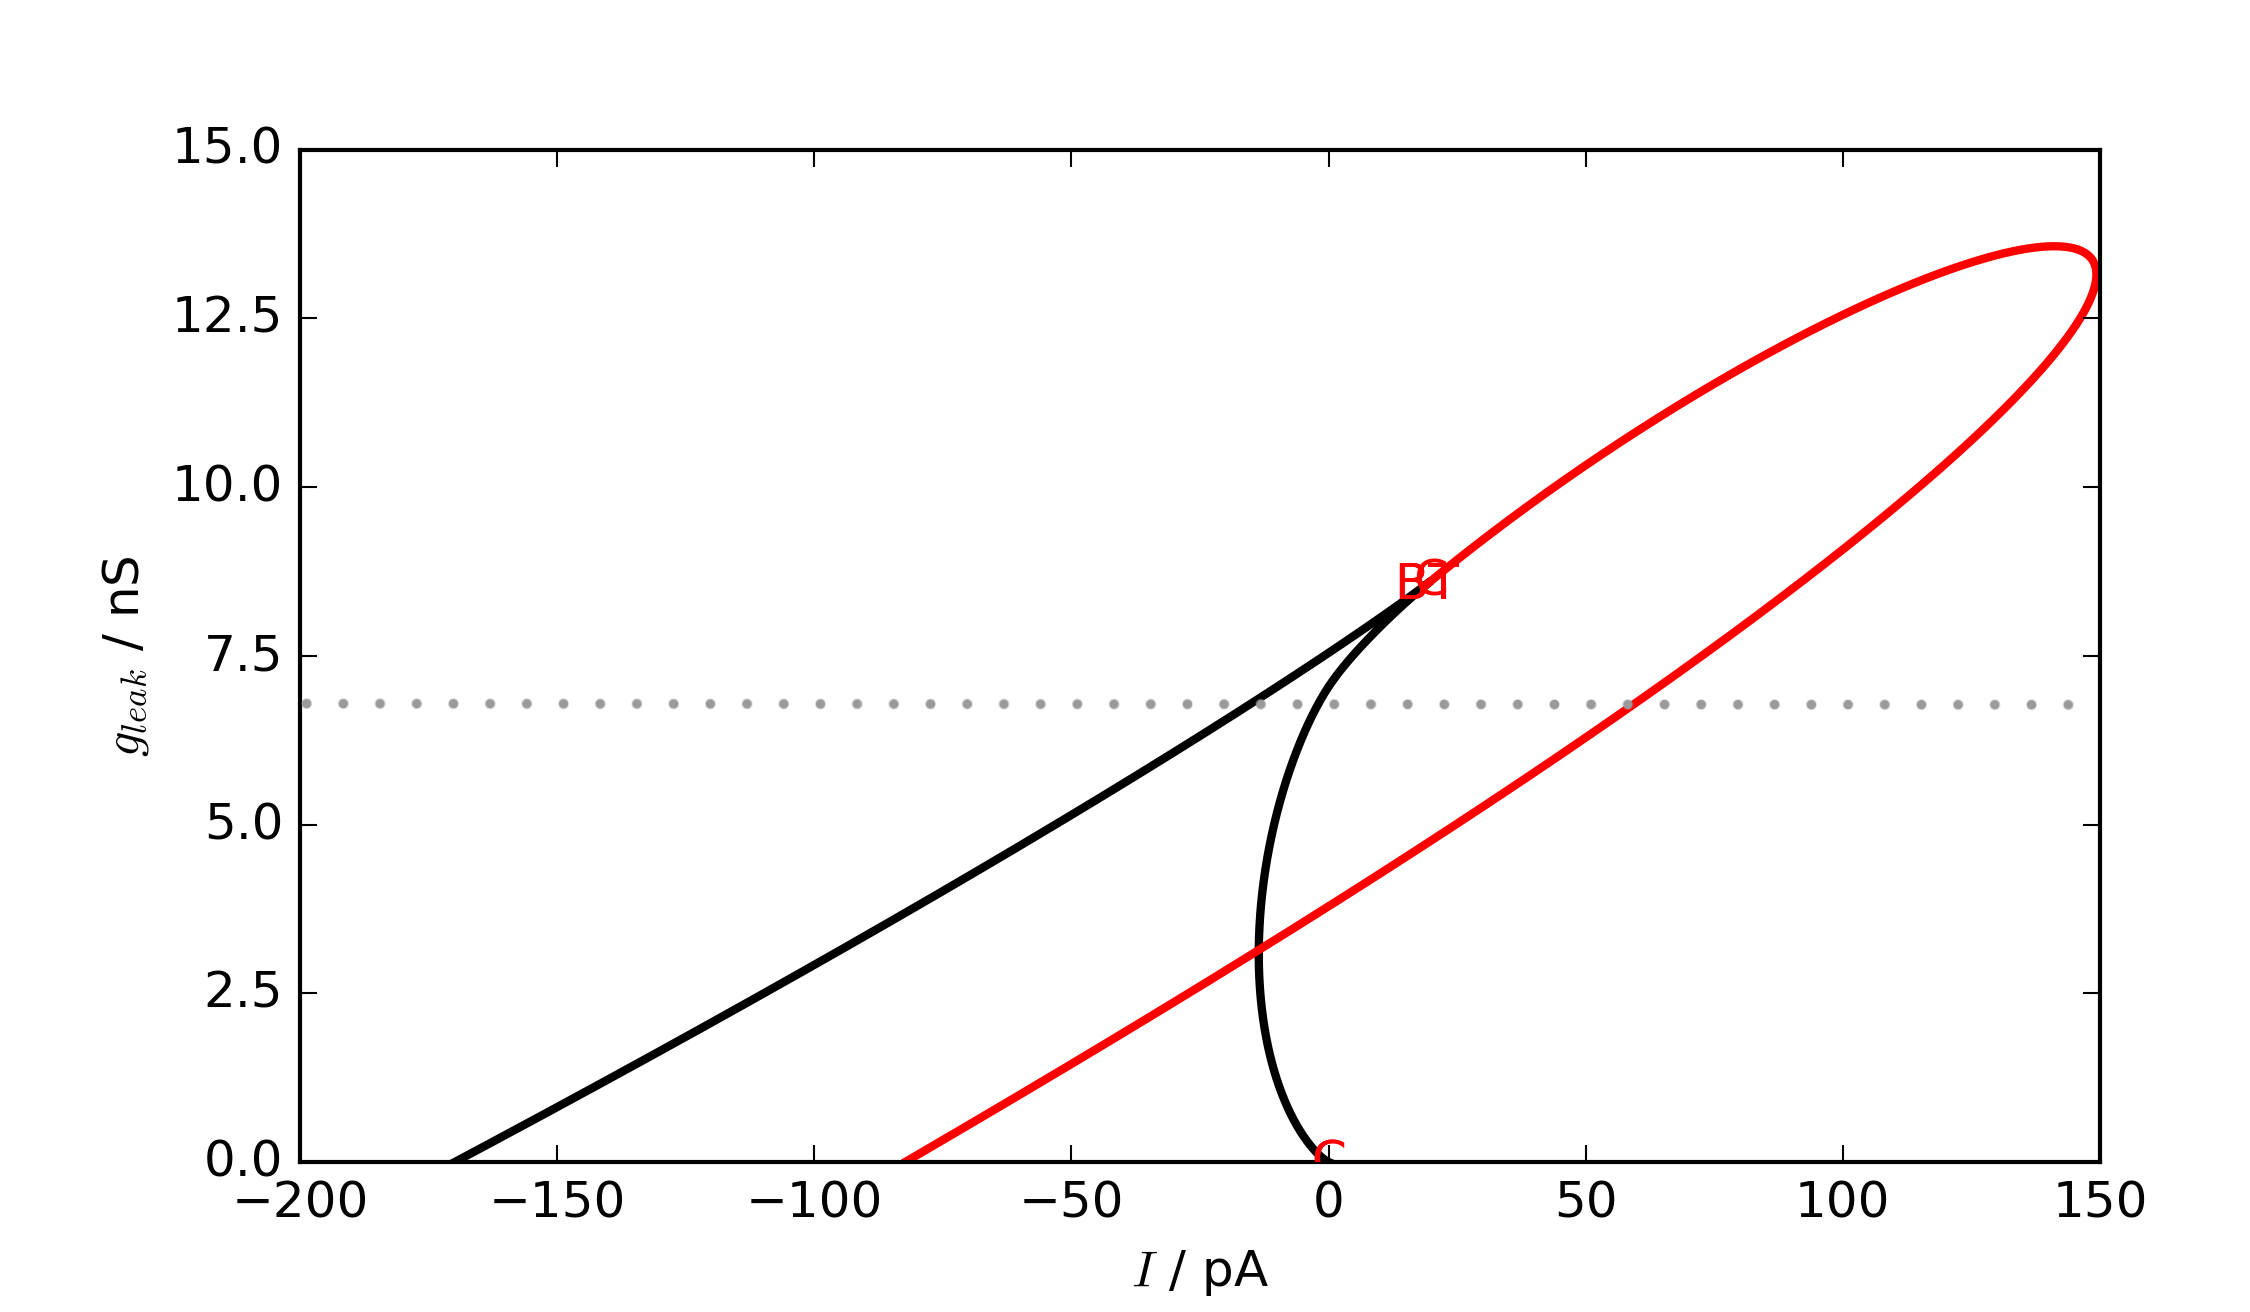
\includegraphics[width=0.500\hsize]{images/2par_gleak.png}}
\\
\subfloat[]{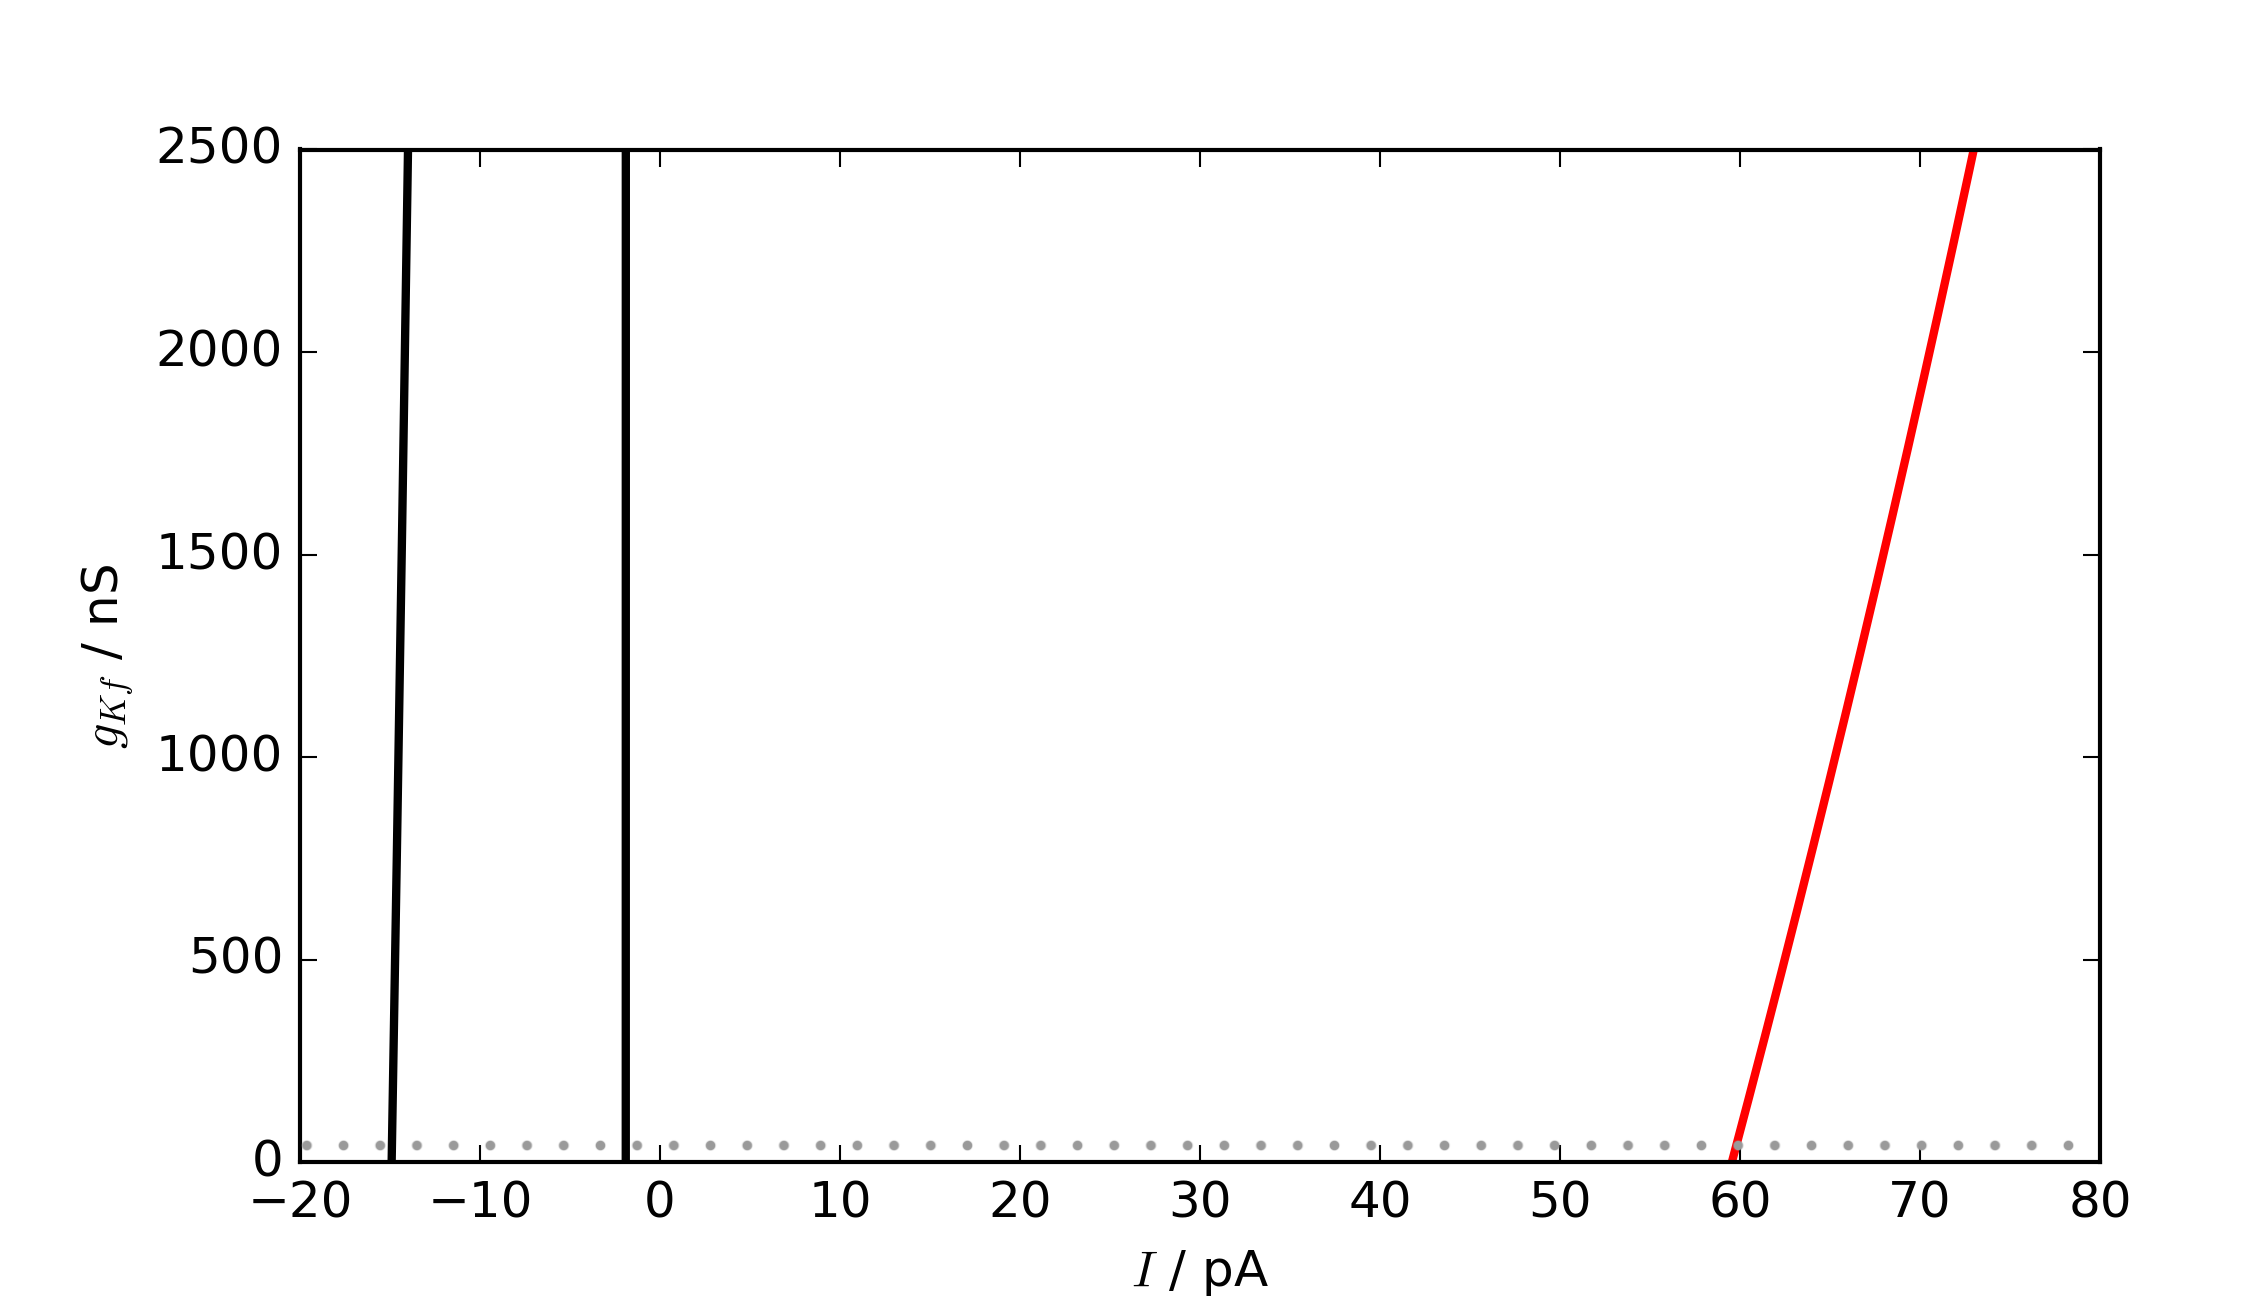
\includegraphics[width=0.500\hsize]{images/2par_gKf.png}}
\subfloat[]{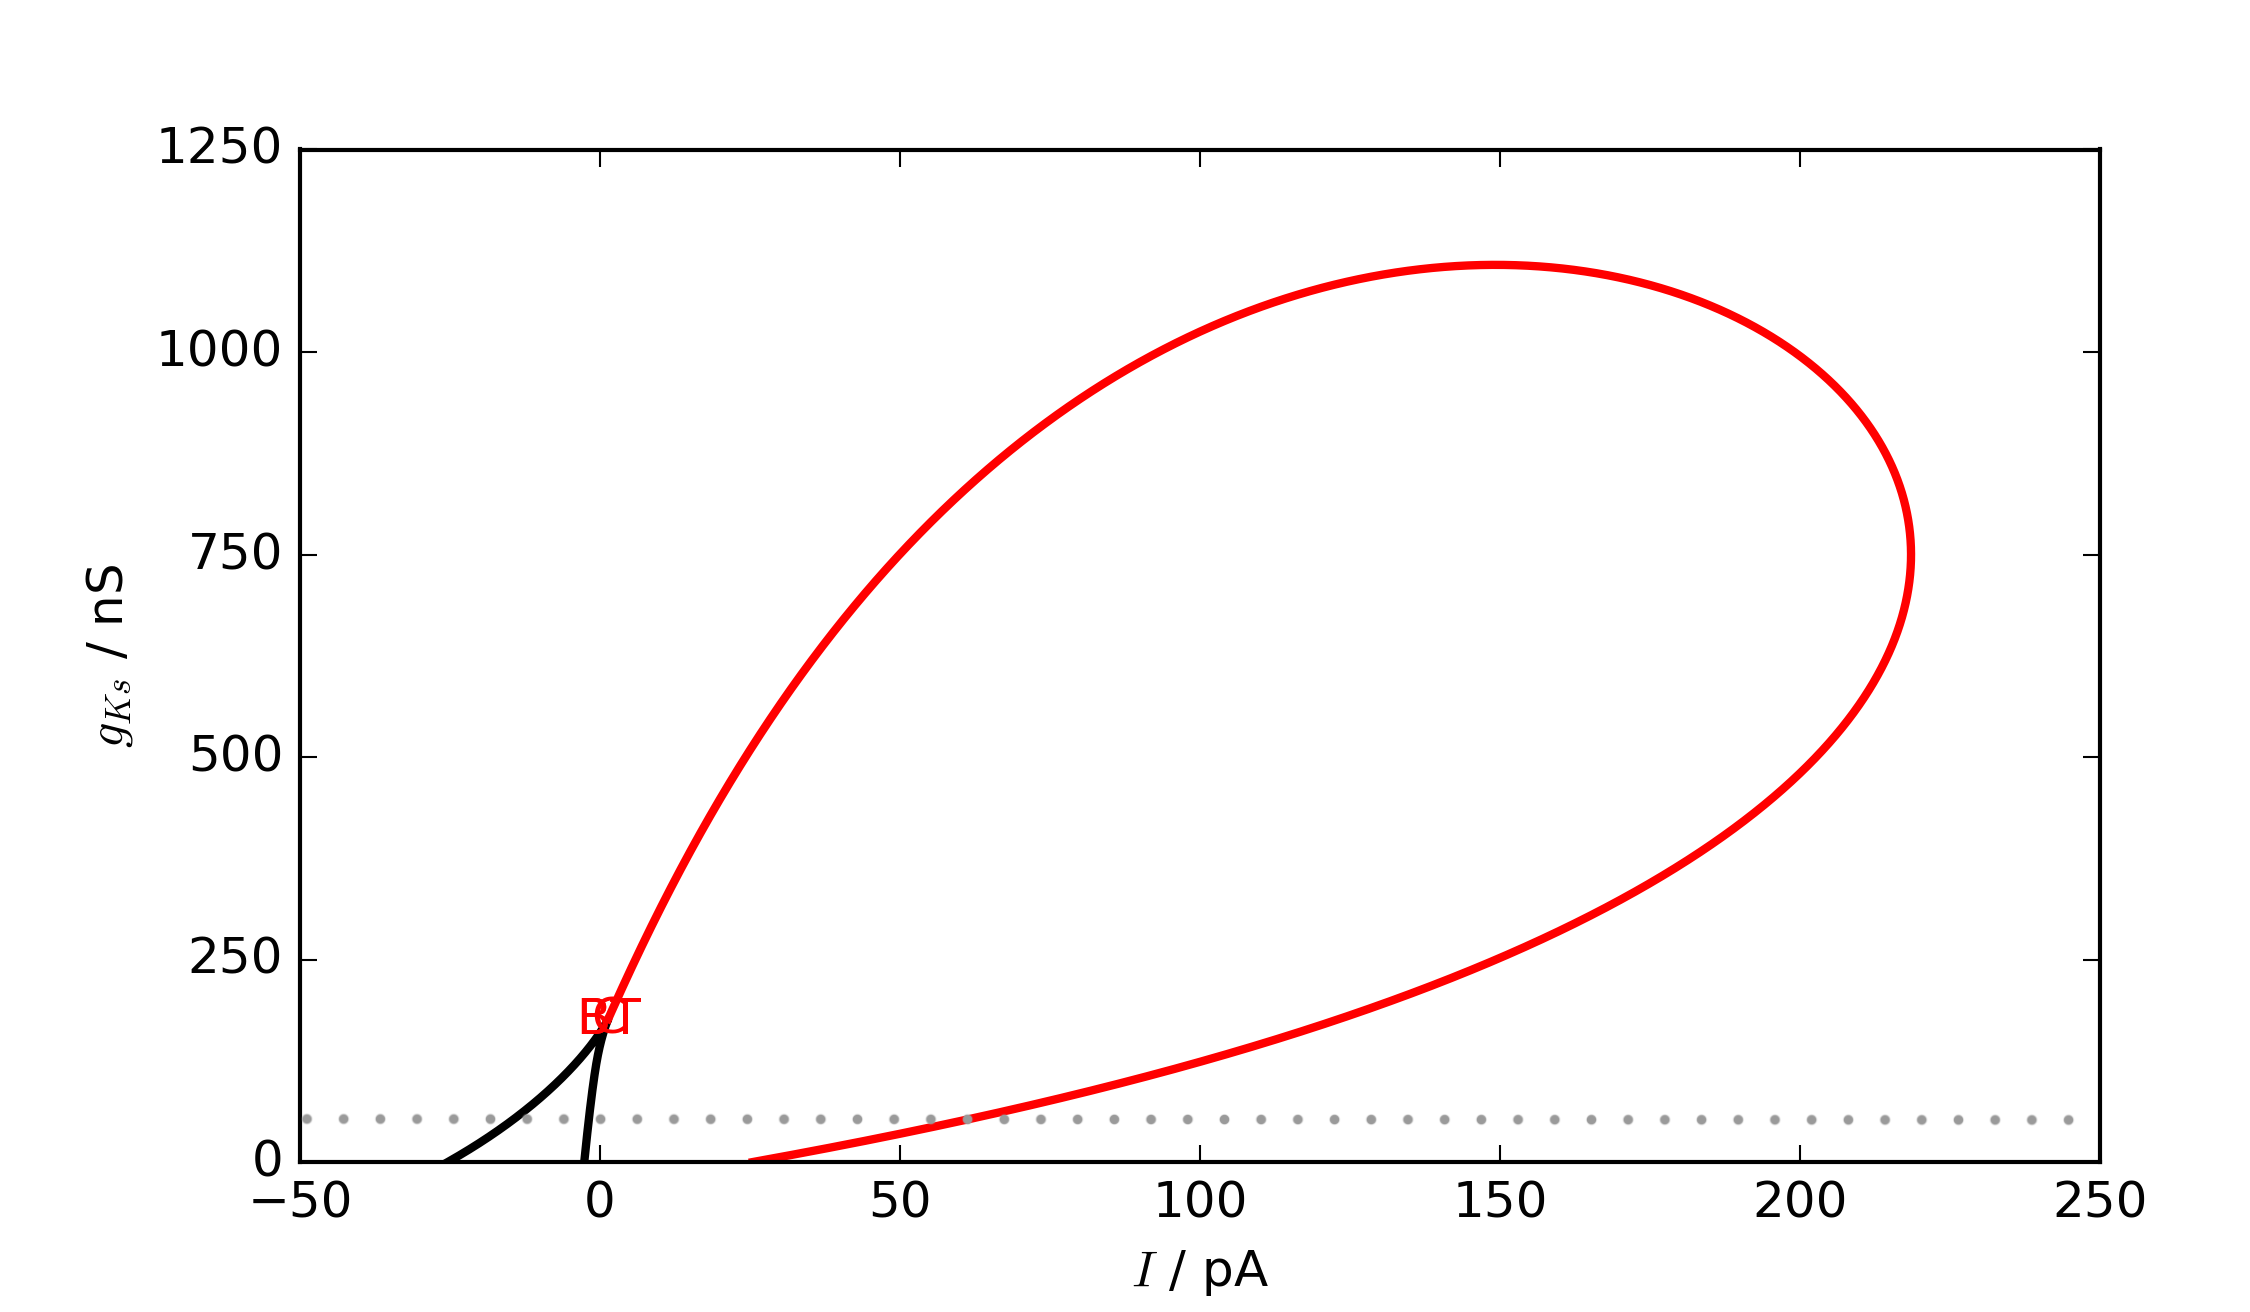
\includegraphics[width=0.500\hsize]{images/2par_gKs.png}}
\\
\subfloat[]{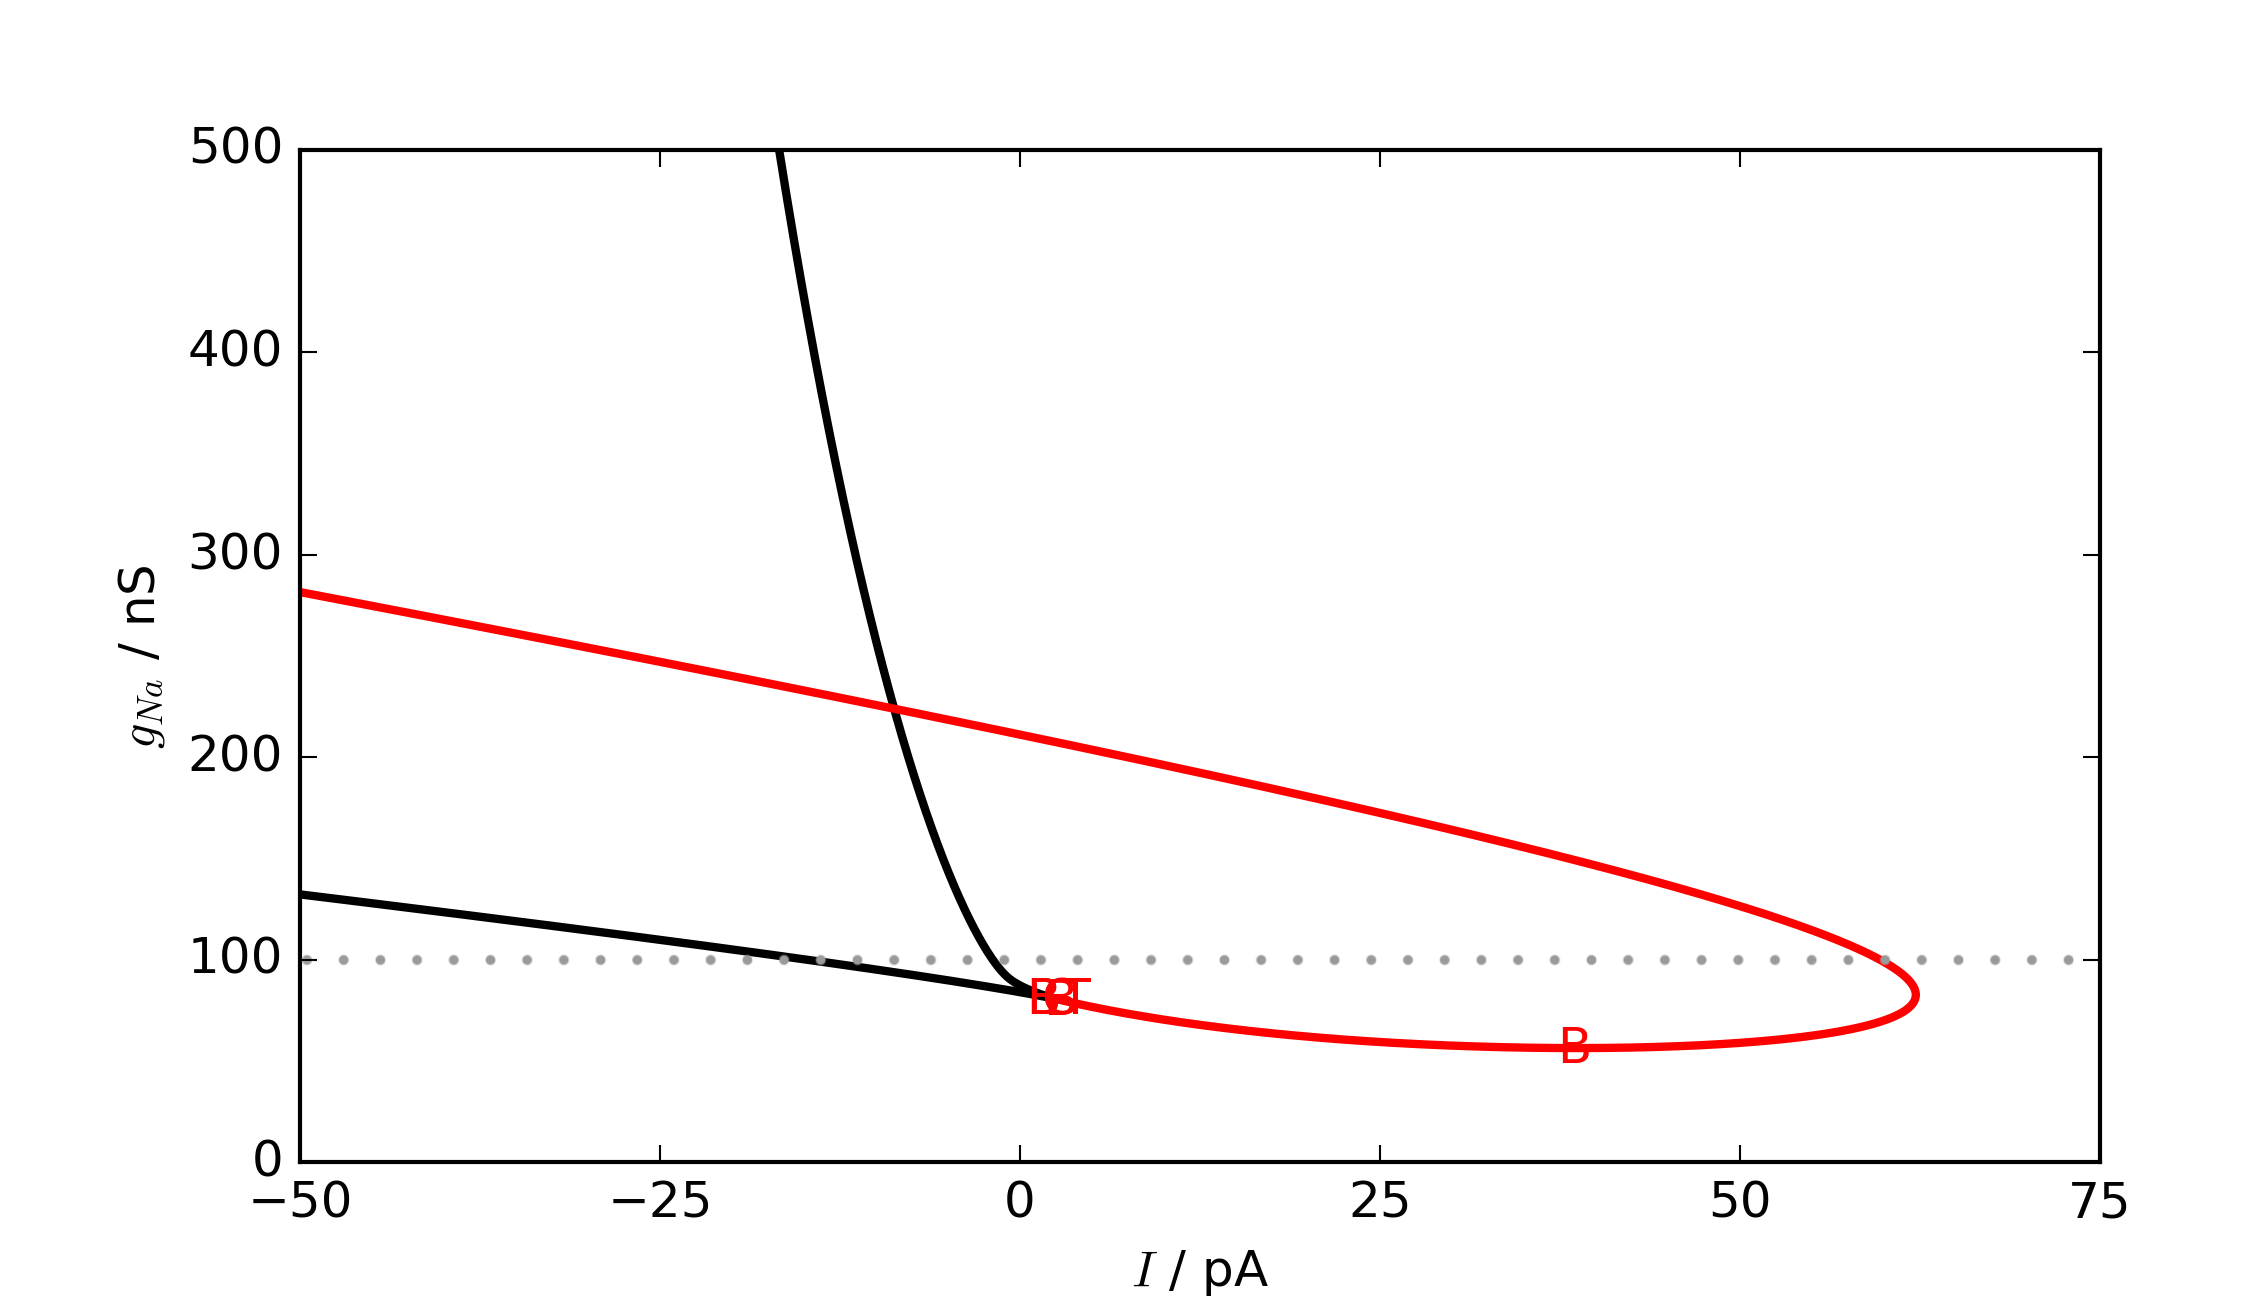
\includegraphics[width=0.500\hsize]{images/2par_gNa.png}}
\subfloat[]{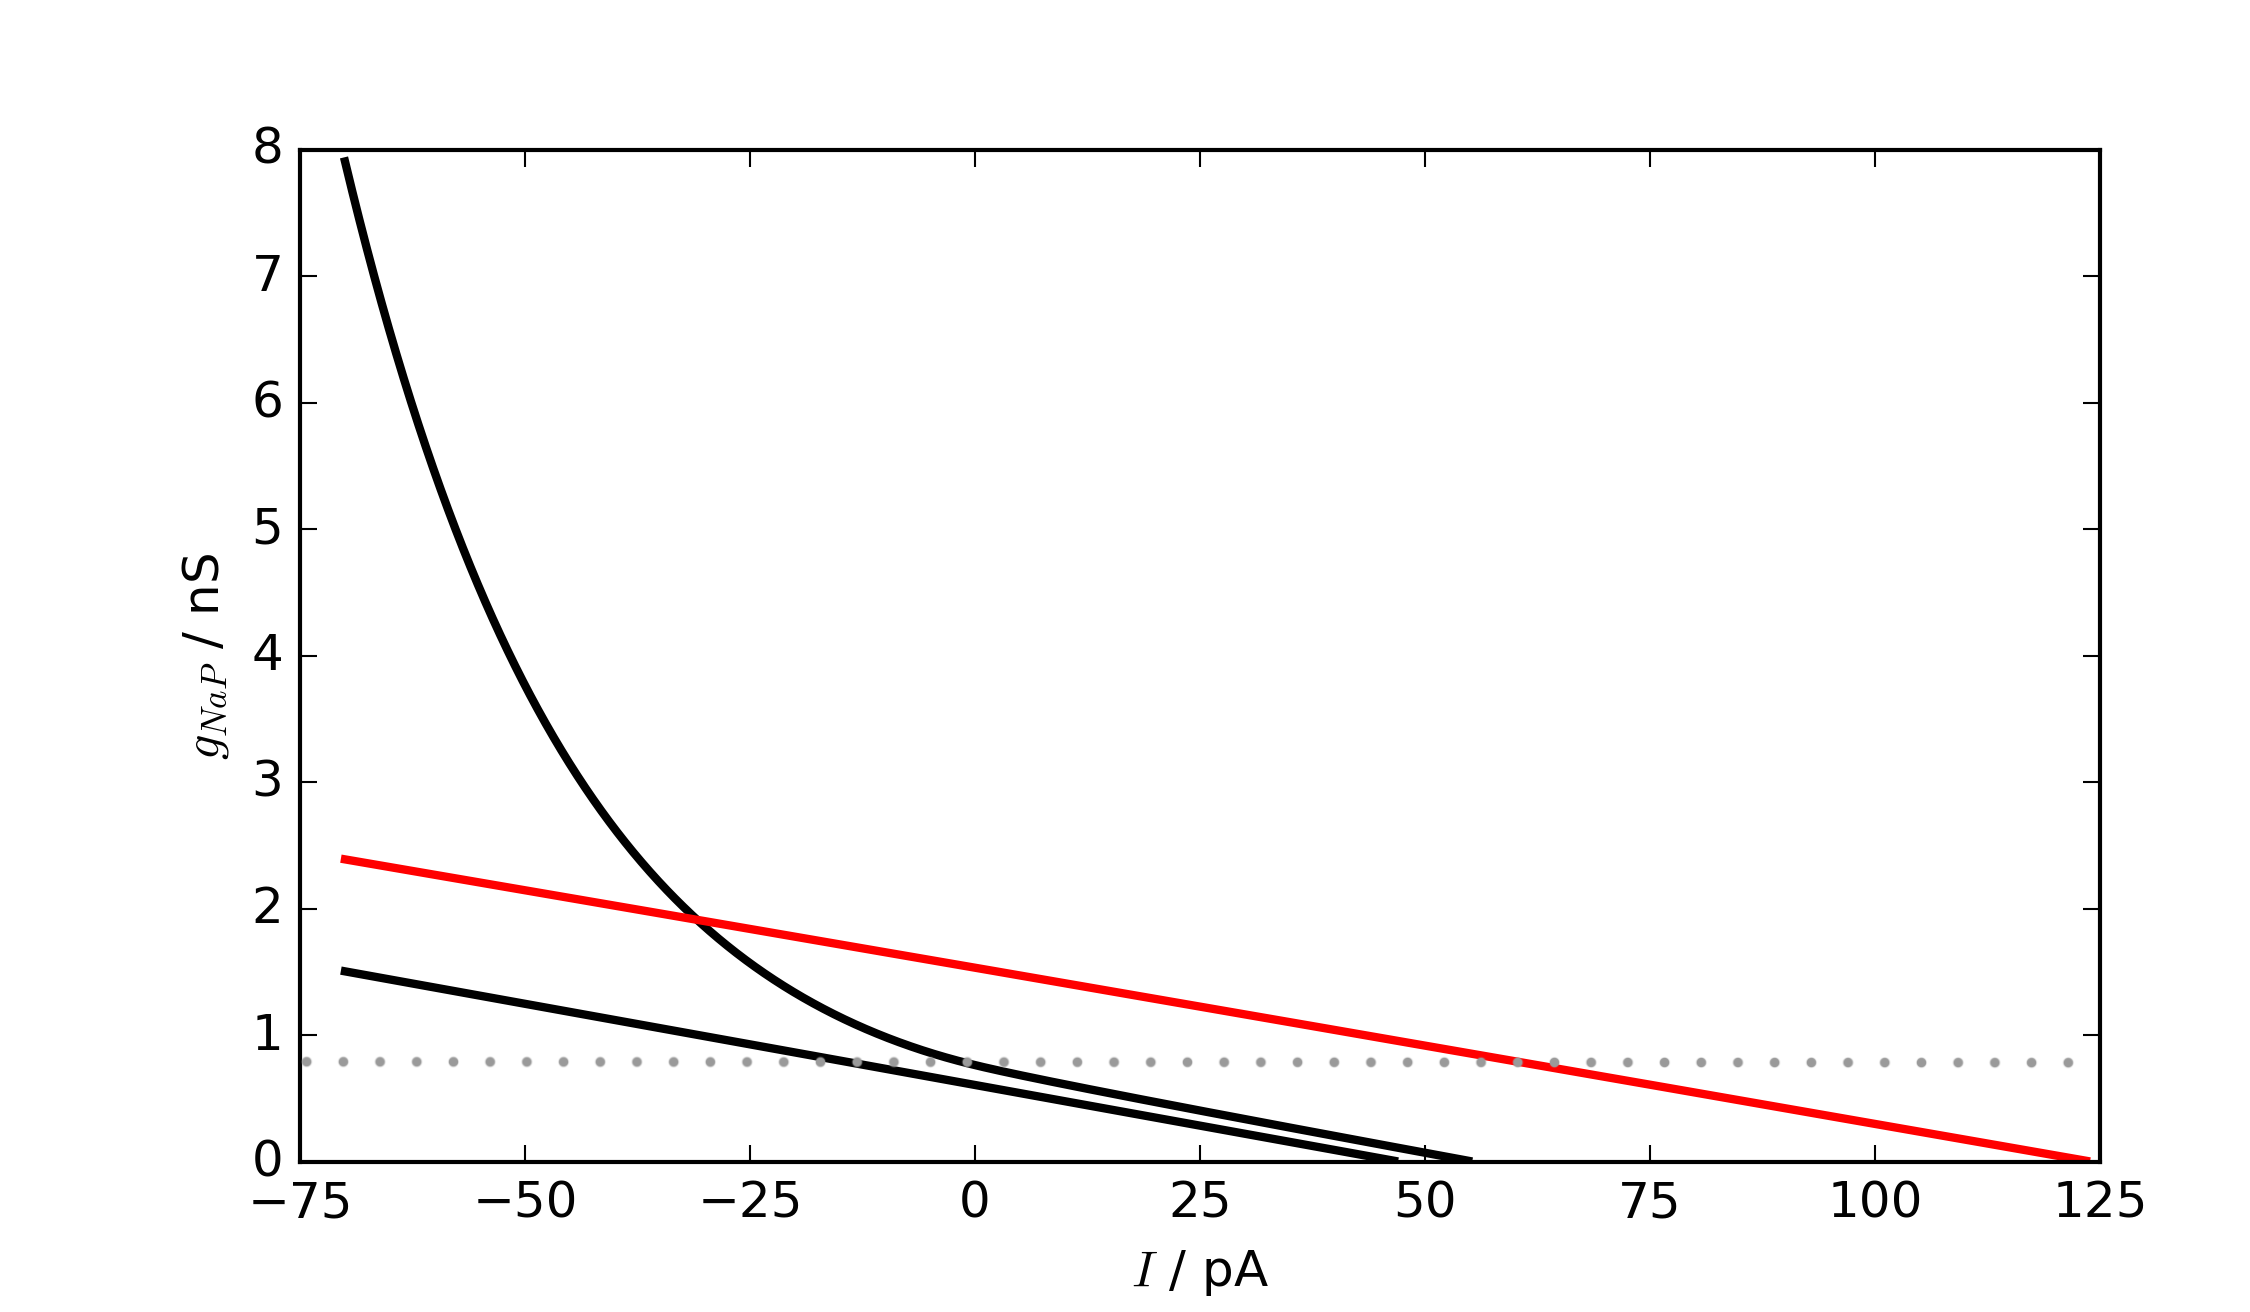
\includegraphics[width=0.500\hsize]{images/2par_gNaP.png}}
\caption[Two-parameter bifurcation diagrams for changing $I$ and one
conductance]{Two-parameter bifurcation diagrams for changing $I$ and one
conductance. Dashed grey line: Default parameter value. Black line:
Saddle-node bifurcation. Red line: Hopf bifurcation. BT: Bogdanov-Takens
bifurcation. C: Cusp bifurcation. B: Bautin
bifurcation.}\label{two-par-cont-plots}
\end{figure}

\subsection{Leak Current}\label{leak-current}

If $g_{leak}$ was decreased from its default value, the codimension-1
bifurcations of the system moved to lower values of $I$. Therefore, the
neuron needed weaker stimuli to start spiking; it became more excitable.
At $g_{leak}$ = 3.14 nS, the saddle-node bifurcation from the onset of
spiking and the Hopf bifurcation from the end of spiking occurred at the
same value of $I$. However, these bifurcations affected different
equilibria (therefore no codimension-2 bifurcation). For very small
values of $g_{leak}$, the saddle-node bifurcation from the onset of
spiking stopped moving to lower values of $I$, and changed direction to
higher values of $I$. Therefore, the S-shape of equilibria from the
(one-parameter) bifurcation diagram in fig.~\ref{bifurcation-diagram}
became more ``stretched''.

If $g_{leak}$ was increased from its default value, the codimension-1
bifurcations moved to higher values of $I$ (i. e. spiking needed
stronger stimuli; less excitable). The two saddle-node points approached
each other. Consequently, the S-shape in the bifurcation diagram
(fig.~\ref{bifurcation-diagram}) became smaller. Eventually, the two
bifurcations merged in a Cusp bifurcation and disappeared. Near this
Cusp bifurcation (for a slightly smaller value of $g_{leak}$), a
Bogdanov-Takens bifurcation was observed. At this point, a subcritical
Hopf bifurcation emanated from the saddle-node bifurcation that controls
the onset of spiking. Additionally, a fold limit cycle bifurcation
appeared (replacing the homoclinic bifurcation), which is consistent
with theory (Izhikevich 2007, p.~195). Consequently, these two
bifurcations dominated the onset of spiking for high values of
$g_{leak}$ (above the Cusp and Bogdanov-Takens bifurcation; see fourth
row in fig.~\ref{bifurcation-combinations}). The end of spiking was
still governed by the supercritical Hopf bifurcation that was observed
for default parameter values (see~\ref{end-of-spiking}).
Fig.~\ref{high-gleak} shows a one-parameter bifurcation diagram for high
$g_{leak}$. It clearly depicts the fold limit cycle bifurcation as well
as the two Hopf bifurcations. At this high value of $g_{leak}$, the
model showed oscillations similar to fig.~\ref{voltage-traces}D in
simulations.

Above the Cusp and Bogdanov-Takens bifurcations, the codimension-1
bifurcations continued to move to higher values of $I$. The distance of
the Hopf bifurcations (in terms of $I$) stayed more or less the same. At
$g_{leak}$ = 13.57 nS, they merged and disappeared. For $g_{leak}$
values above this point, the system lacked a limit cycle. Therefore, it
showed silent behaviour for arbitrary current stimuli.

\begin{figure}
\centering
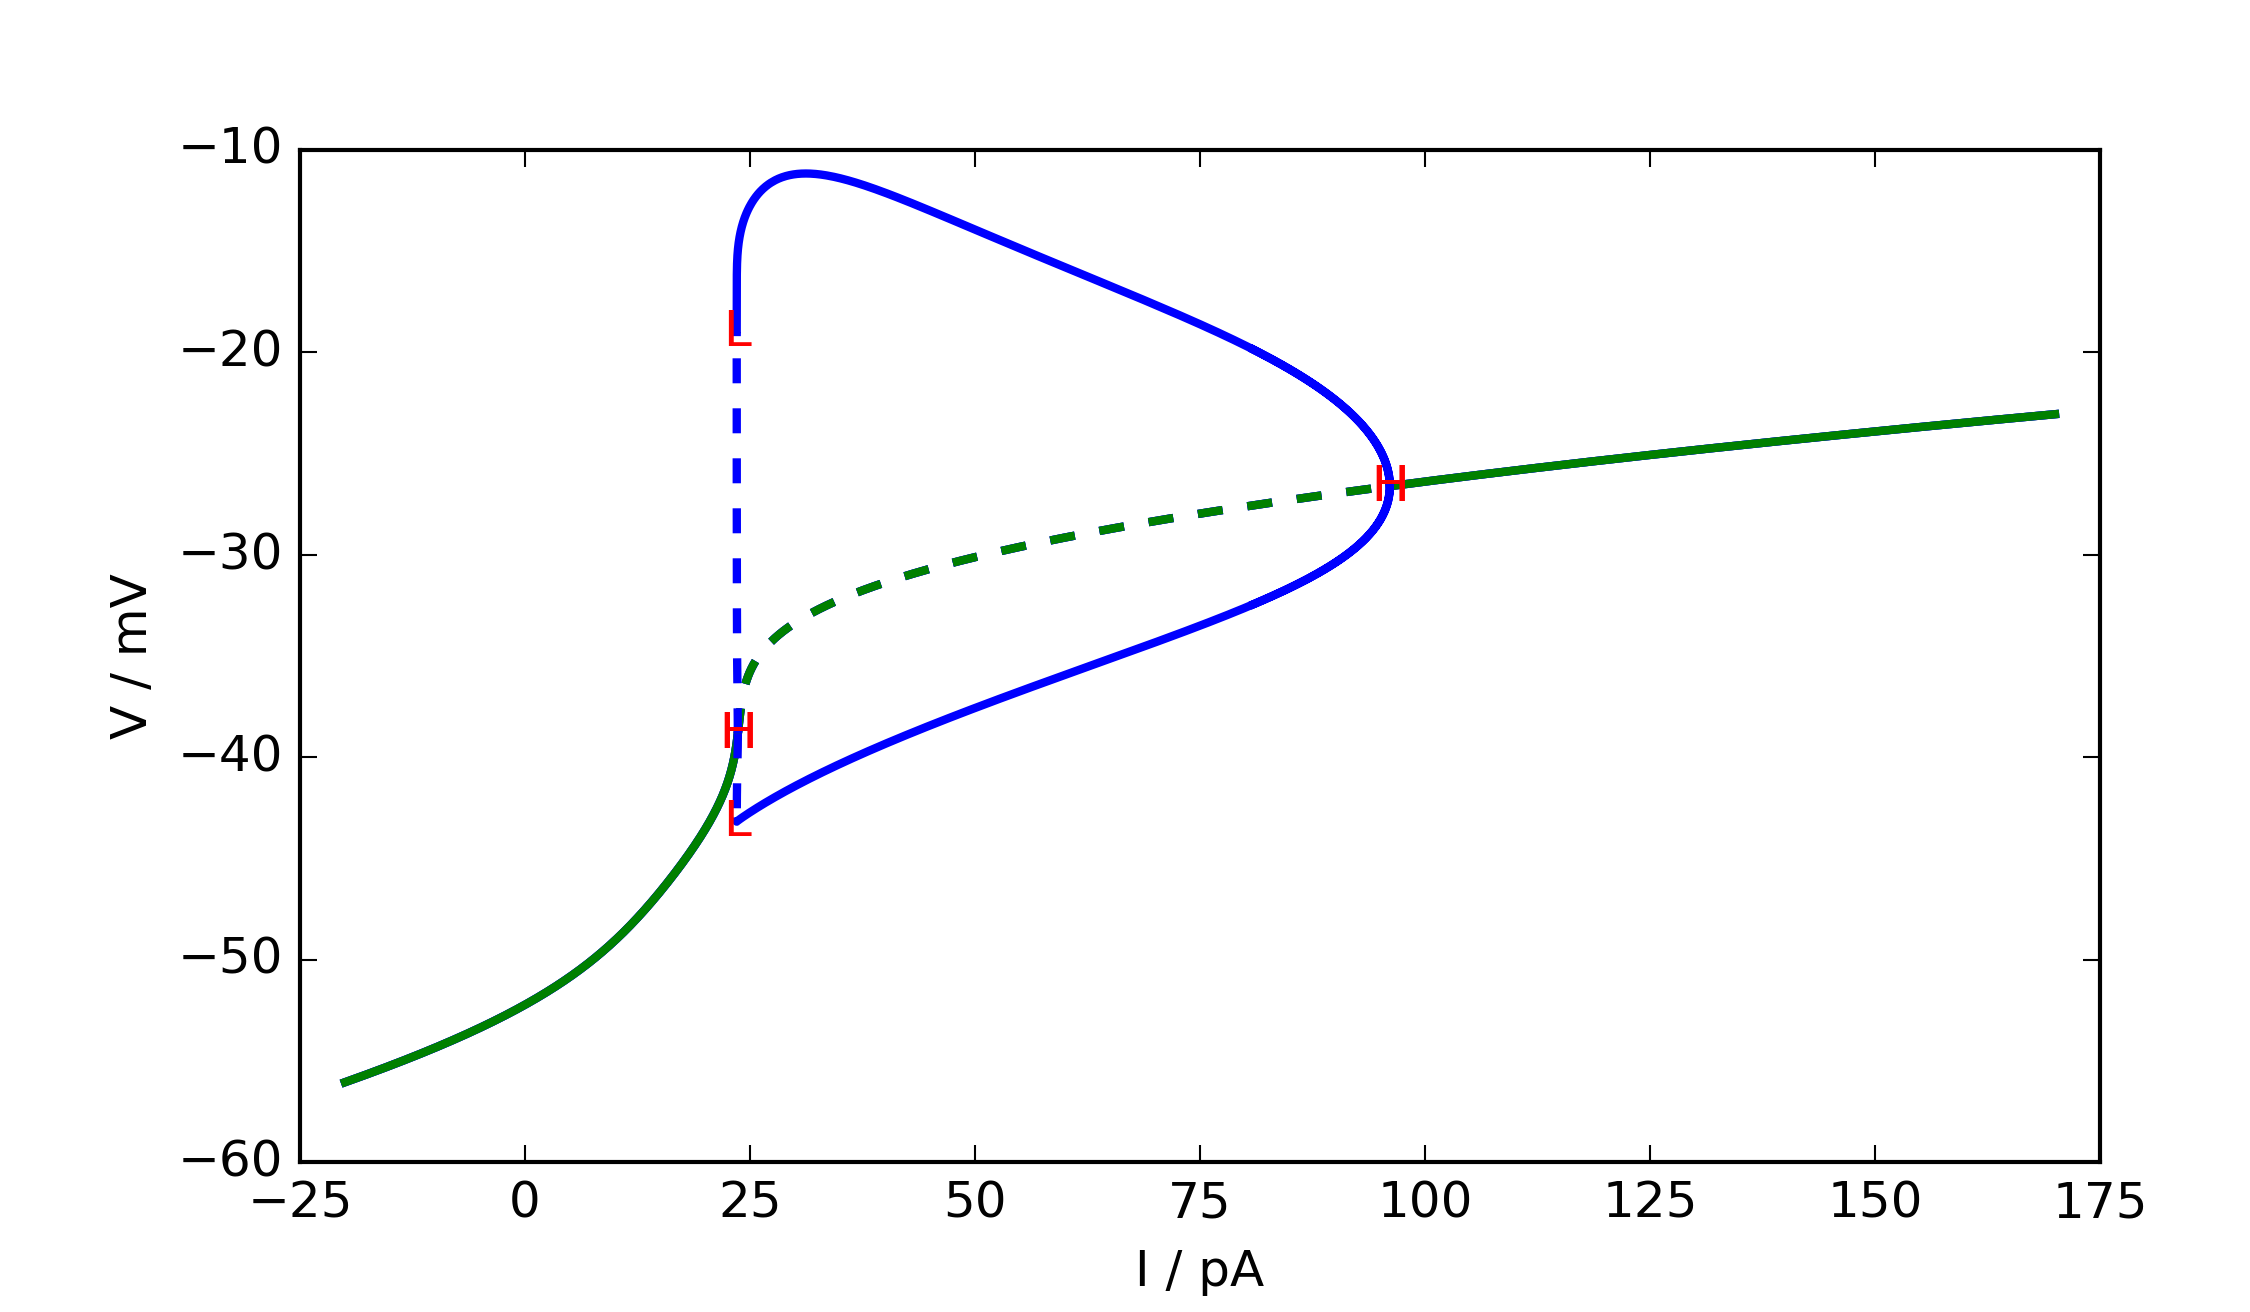
\includegraphics[]{images/bifurcation_gleak=8.84.png}
\caption[Bifurcation diagram for changing $I$ at high $g_{leak}$]{Bifurcation diagram for changing $I$ at high $g_{leak}$
(8.84 nS). Green solid line: Stable equilibrium. Green dashed line:
Unstable equilibrium. Blue line: Minimum/maximum of limit cycle. H: Hopf
bifurcation. L: Fold limit cycle bifurcation.}\label{high-gleak}
\end{figure}

\subsection{Fast Potassium (Kf)
Current}\label{fast-potassium-kf-current}

Changing $g_{Kf}$ hardly affected the codimension-1 bifurcations of the
system, even if it was increased 100-fold, or set to zero. Only the
supercritical Hopf bifurcation at the end of spiking moved slightly in
terms of $I$. Therefore, the behaviour of the neuron stayed more or less
the same for changes of $g_{Kf}$.

\subsection{Slow Potassium (Ks)
Current}\label{slow-potassium-ks-current}

The two-parameter continuation for $g_{Ks}$ showed similarities to
gleak. This is plausible because both currents are inward, and should
therefore have a similar effect on model behaviour. For smaller values
of $g_{Ks}$ than default, all codimension-1 bifurcations moved to lower
values of $I$. Therefore, the neuron needed weaker stimuli to start
spiking and became more excitable. In contrast to $g_{leak}$, the
saddle-node bifurcation from the onset of spiking kept moving to lower
values of $I$ throughout the continuation, and did not change direction
at some point.

For values of $g_{Ks}$ higher than default, all bifurcations moved to
the right, and the neuron became less excitable. The two saddle-node
bifurcations approached each other and merged in a Cusp bifurcation. As
with $g_{leak}$, a Bogdanov-Takens bifurcation occurred just before this
Cusp bifurcation. It created a subcritical Hopf bifurcation and a fold
limit cycle bifurcation. For high $g_{Ks}$, the onset of spiking was
dominated by these two bifurcations. The one-parameter bifurcation
diagram looked similar to the one for high $g_{leak}$
(fig.~\ref{high-gleak}).

For even higher values of $g_{Ks}$, all bifurcations moved to higher
values of $I$. The two Hopf bifurcations moved away from each other (in
terms of $I$). Therefore, the neuron spiked repeatedly for a wider range
of current stimuli. For very high $g_{Ks}$, the Hopf bifurcations
converged and eventually merged and disappeared (compare high
$g_{leak}$). Above $g_{Ks}$ = 1107.57 nS, the system showed a stable
equilibrium and silent behaviour for arbitrary current inputs.

\subsection{Transient Sodium (Na)
current}\label{transient-sodium-na-current}

For lower values of $g_{Na}$ than default, the bifurcations of the
system moved to higher values of $I$, i. e. the neuron became less
excitable. At $g_{Na}$ = 80.23 nS (i. e. if it was decreased by one
fifth), the saddle-node points merged in a Cusp bifurcation. Slightly
before this bifurcation, a Bogdanov-Takens bifurcation occurred and
created a Hopf bifurcation. In contrast to high $g_{leak}$ and high
$g_{Ks}$, this Hopf bifurcation was supercritical at first. Therefore,
at this point the stable limit cycle of the system was created as well
as destroyed by a supercritical Hopf bifurcation. However, the new Hopf
bifurcation became subcritical at a slightly lower value of $g_{Na}$
through a Bautin bifurcation. Additionally, the system now showed a fold
limit cycle bifurcation. Therefore, at low values of $g_{Na}$ the onset
of spiking was governed by the same mechanism as for high $g_{leak}$ and
high $g_{Ks}$ (fig.~\ref{high-gleak}).

For even lower values of $g_{Na}$, the two Hopf bifurcations converged.
Eventually, they merged in a Bautin bifurcation (which is ``needed'' to
connect the loci of the subcritical and supercritical Hopf
bifurcations).

For high $g_{Na}$, all bifurcations of the system moved to smaller
values of $I$, i. e. the neuron became more excitable. The saddle-node
bifurcation from the onset of spiking moved more slowly. At $g_{Na}$ =
223.85 nS, it occurred at the same value of $I$ as the supercritical
Hopf bifurcation from the end of spiking.

\subsection{Persistent Sodium (NaP)
current}\label{persistent-sodium-nap-current}

For lower values of $g_{NaP}$ than default, all bifurcations moved to
higher values of $I$. Thus, the neuron became less excitable. The two
saddle-node bifurcations slightly approached each other, but always
occurred at different values of $I$.

For high values of $g_{NaP}$, all bifurcations moved to lower values of
$I$. The saddle-node bifurcation from the onset of spiking moved only
slowly and almost stayed at the same value of $I$ for very high
$g_{NaP}$. At some point, it occurred at the same value of $I$ as the
Hopf bifurcation from the end of spiking.

\chapter{Discussion}\label{discussion}

In this study, an isopotential model of the MN1-Ib motoneuron in
\emph{Drosophila} was investigated for its dynamics. In simulations, the
model exhibited four different types of behaviour and diverse spiking
properties. These effects were explained by three distinct bifurcations
of codimension 1. Subsequently, it was shown how the bifurcations (and
therefore the behaviour) of the model change if the strengths of its ion
currents are altered.

\section{Comparison to Experiments}\label{comparison-to-experiments}

In the simulations performed for this thesis
(see~\ref{qualitative-behaviour}), the model showed similar qualitative
behaviour as in experiments (current-clamp recordings of abdominal and
thoracic MN1-Ib neurons in Choi 2004, Hartwig 2008, Schaefer 2010):
Silent behaviour for weak stimuli, a clear rheobase current, and regular
tonic spiking above the rheobase (no single spikes, no adaptation). The
bistability of the model in region B is not reported experimentally.
However, this feature only persists for a small range of current stimuli
(\textless{} 1 pA). Therefore, it was possibly overlooked in
experimental setups, which typically stimulate the neuron in 20-pA-steps
(Choi 2004, Schaefer 2010).

For strong stimuli, the behaviour in simulations differs from
experiments. While the isopotential model was silent for currents above
59.70 pA (due to a Hopf bifurcation), the experiments consistently show
that MN1-Ib keeps spiking for strong currents (at least up to 100 pA).
Accordingly, the oscillations of the model in region D (above the Hopf
bifurcation) were not observed in experiments. However, some recordings
from the MN5 neuron in (adult) \emph{Drosophila} (Herrera-Valdez 2013,
Berger 2015) show a similar behaviour to the MN1-Ib model near the Hopf
bifurcation (tonic spiking below, oscillations above the bifurcation).
This makes it at least plausible that a similar behaviour may exist in
MN1-Ib at very high current stimuli.

In addition to qualitative behaviour, simulations and experiments
roughly agree in terms of values for resting potential, rheobase, firing
rates and delays. However, these values exhibit a strong variation in
experiments (Choi 2004, Hartwig 2008, Schaefer 2010, Günay 2015), which
may be attributed to differences in the experimental setups as well as
natural neuron variability. This variability of MN1-Ib is consistent
with other motoneurons in \emph{Drosophila}, for example MN5
(Herrera-Valdez 2013). Therefore, comparing the exact values has a
limited validity.

In detail, the resting potential derived from simulations (-54.56 $\pm$
0.01) mV) lies in the same range as the values from experiments ((-56
$\pm$ 1) mV in Choi 2004, (-46.6 $\pm$ 1.3) mV in Schaefer 2010).
However, the resting potential of the model is obviously determined by
the default bias current of -12 pA. By tweaking this current slightly,
the resting potential can be easily adjusted to any value between -50 mV
and -60 mV (compare stable equilibrium in
fig.~\ref{bifurcation-diagram}).

The rheobase of the model ((10.10 $\pm$ 0.01) pA in relation to the bias
current) is rather low in comparison to experiments ((27 $\pm$ 5) pA in
Choi 2004, (45 $\pm$ 3) pA in Schaefer 2010). However, these
experimental findings could be slightly biased towards higher values:
Usually, the stimulation protocols use current steps of 0 pA, 20 pA, 40
pA, etc. to determine the rheobase. Therefore, neurons with low rheobase
currents (say 5 pA) would still show quite large values in these
experiments (at least 20 pA). Additionally, the rheobase currents of
individual neurons varied significantly in experiments.

Concerning spike properties, the qualitative features from simulations
and experiments are in agreement. In brief, current clamp recordings
showed that firing rate increases with stimulus strength (Schaefer 2010,
Hartwig 2008), while delay to first spike decreases (Schaefer 2010, Choi
2004). The exact curves vary across studies and neurons. A comparison of
firing rate and delay between the isopotential model and recordings is
already given in Günay 2015 (see fig. 2B and C in there). The
simulations for this thesis (fig.~\ref{f-i-curve} and~\ref{plot-delays})
replicate these results and extend the resolution and range in terms of
the stimulus current $I$. As stated in~\ref{mn1-ib-model} and Günay
2015, the isopotential model fails to reproduce the correct spike shape
and amplitude of the MN1-Ib neuron. Considering the phase portrait, this
means that the properties of the limit cycle are wrong.

\section{Computational Properties}\label{computational-properties}

For default parameter values, the model showed typical integrator
properties in simulations (clear threshold and rheobase, no
oscillations). This is in agreement with the properties of MN1-Ib
observed \emph{in vivo} (see~\ref{comparison-to-experiments}).
Bifurcation analysis unveiled that the onset of spiking is governed by
subsequent fold limit cycle and saddle-node bifurcation. This
combination of bifurcations causes the integrator behaviour
(\ref{integrators-and-resonators}). For strong current stimuli, the
system showed a supercritical Hopf bifurcation and oscillations as a
typical resonator property. However, this behaviour is limited to strong
stimuli and does not have a major impact on tonic spiking. Therefore,
its effect on the computational properties of the neuron is likely
small. Also, the Hopf bifurcation and oscillations were not observed
experimentally (see~\ref{comparison-to-experiments}).

The computational properties of a neuron can change for different
parameter values. More specifically, a Bogdanov-Takens bifurcation
switches between integrator and resonator behaviour (Izhikevich 2007,
pp.~195-196 and 251). As shown by two-parameter continuation
(see~\ref{two-par-cont}), the MN1-Ib model undergoes a Bogdanov-Takens
bifurcation for changes in $g_{leak}$, $g_{Ks}$ and $g_{Na}$. In all cases, the
Bogdanov-Takens bifurcation occurred near a Cusp bifurcation. Together,
these two bifurcations change the mechanism behind the onset of spiking
from a saddle-node bifurcation to a Hopf bifurcation, and therefore from
integrator to resonator properties. Hence, the neuron model is a
resonator for high $g_{leak}$, high $g_{Ks}$ and low $g_{Na}$. For changes in $g_{Ks}$ and
$g_{NaP}$, no Bogdanov-Takens or Cusp bifurcations were observed.
Nevertheless, experiments did not show any resonating properties for
MN1-Ib (Choi 2004, Schaefer 2010, Hartwig 2008). Therefore, it is
questionable whether MN1-Ib ever reaches the parameter values necessary
for a Bogdanov-Takens bifurcation \emph{in vivo}. Also, it is unclear
whether it would make sense for a motoneuron to show resonating
behaviour (considering its role as an integrator for signals from the
CPG and other circuits).

\section{Role of Ion Currents}\label{role-of-ion-currents}

The neuron model in this thesis contains a passive leak current, two
outward potassium currents (fast Kf and slow Ks), and two inward sodium
currents (transient Na and persistent NaP). To show how each current
influences the model behaviour, two parameter continuation of the
respective conductances was employed (see~\ref{two-par-cont}).

\subsection{Comparison of Inward and Outward
Currents}\label{comparison-of-inward-and-outward-currents}

Stronger outward currents (Ks, Kf, leak) and weaker inward currents (Na,
NaP) made the neuron less excitable (i. e. the bifurcations moved to
higher values of $I$ and the neuron needed stronger stimuli to
transition to spiking behaviour). Conversely, weaker outward currents
and stronger inward currents made the neuron more excitable. This is
expected from a biophysical point of view: To start spiking, the neuron
needs a strong inward current (usually sodium). Therefore, inward
currents promote spiking, while outward currents prevent it. Using the
two-compartmental version of the MN1-Ib model (see~\ref{mn1-ib-model}),
Lin 2012 showed that strong NaP increases the excitability of the neuron
(and thus promotes seizure behaviour). This is consistent with the
results from the isopotential model presented in this thesis.

The currents Ks, Na and leak had a strong impact on model behaviour.
Especially, varying these currents produced codimension-2 bifurcations,
which switch the computational properties of the neuron
(see~\ref{computational-properties}). In contrast, the impact of NaP was
weak and the impact of Kf almost negligible. As these currents are
already weak in the default model, it is plausible that they do not have
a major influence on the behaviour of MN1-Ib. This view is supported by
Herrera-Valdez 2013, who constructed a minimal model of the MN5 neuron
in (adult) \emph{Drosophila}. It contains a leak current, one potassium
current similar to Ks, and one sodium current (i. e. all currents that
play a major role in the MN1-Ib model). Despite its simplicity, their
model was able to replicate all experimentally observed behaviours of
MN5, including tonic spiking and oscillations. In summary, a slow
potassium current (like Ks) and a transient sodium current (like Na)
seem to be the major (active) driving forces of behaviour in
\emph{Drosophila} motoneurons like MN1-Ib and M5.

\subsection{Role of Potassium Currents for
Spiking}\label{role-of-potassium-currents-for-spiking}

Experimentally, the ion currents in MN1-Ib can be altered through
genetic manipulation of the underlying ion channels. Hartwig 2008
present recordings from \emph{Drosophila} larvae with decreased (EKI
manipulation) and increased (EKO manipulation) potassium currents. For
both manipulations, the MN1-Ib neuron showed a similar resting potential
and firing threshold as in wild-type larvae. This seems to be consistent
with the results from the two-parameter continuation for $g_{Ks}$ and
$g_{Kf}$: In both cases, the saddle-node bifurcation at the onset of
spiking stayed at more or less the same value of $I$ for (moderate)
changes of the conductance (fig.~\ref{two-par-cont-plots}). Therefore,
the stable equilibrium (which determines the resting potential) as well
as the unstable equilibrium (which determines the firing threshold)
should keep their location in phase space.

\subsection{Role of the Kf Current for Spike
Delays}\label{role-of-the-kf-current-for-spike-delays}

In simulations, the MN1-Ib neuron showed a significant delay to first
spike, especially near the onset of spiking (see~\ref{delays}). This
property is also reported in experimental setups for MN1-Ib as well as
other motoneurons in \emph{Drosophila} (Choi 2004, Schaefer 2010).
\emph{In vivo}, the delays seem to play a critical role for muscle
behaviour: They control the recruitment order of motoneurons. For
example, the body wall muscle 1 is innervated by MN1-Ib and MNISN-Is.
The latter motoneuron shows a longer spike delay than MN1-Ib. As both
neurons seem to receive the same synaptic input, the muscle is first
activated by MN1-Ib and then (due to the longer delay) by MNISN-Is
(Schaefer 2010).

Experiments with \emph{Drosophila} motoneurons indicate that a transient
(A-type) potassium current plays a critical role for spike delays (Choi
2004, Schaefer 2010, Srinivasan 2012). This current is encoded by the
\emph{Shal} gene (Tsunoda 1995) and corresponds to Kf in the MN1-Ib
model. From the dynamical systems point of view, the mechanism behind
the spike delay in MN1-Ib is clear: The saddle-node bifurcation at the
onset of spiking creates a region in the phase space, where the
trajectory of the system moves very slowly (see~\ref{delays}). This
implies that the neuron should be able to exhibit spike delays as long
as there is a saddle-node bifurcation - regardless of the underlying
currents, and especially the existence of an A-type potassium current.
The results of this thesis support this view: Firstly, the MN1-Ib model
exhibits long delays even though its Kf current is very weak. Secondly,
changing the strength of the Kf current did not have a significant
effect on the saddle-node bifurcation at the onset of spiking (as shown
by the two-parameter continuation in fig.~\ref{two-par-cont}).

If the A-type current would not play a significant role for spike
delays, how could the results from experiments be explained? Firstly,
some experiments show that spike delays decrease in \emph{Drosophila}'s
motoneurons if the A-type potassium current is blocked (by the drug
4-AP; Choi 2004) or disabled (by RNAi knockdown; Schaefer 2010,
Srinivasan 2012). However, decreasing this current also reduces the
excitability of the neuron, i. e. the bifurcations of the system move to
lower values of $I$ (the two parameter continuation in
fig.~\ref{two-par-cont-plots} indicates this only slightly, as the Kf
current is very weak in this model). Therefore, the spike delays should
also occur at lower current stimuli. If the neuron is stimulated with
the same currents as before (as in the experimental setups), the delays
seem decreased even though they have just moved to different values of
$I$. Secondly, it was found that spike delays decrease in response to
prepulses. These current stimuli are applied before the actual current
step that causes spiking (Choi 2004, Schaefer 2010). Prepulses are known
to inactivate A-type currents (Choi 2004). However, they also bring the
phase space of the neuron close to the saddle-node bifurcation. This is
supported by Choi 2004, who report a membrane potential of (-43 $\pm$ 1) mV
during the prepulse (which should be close to the saddle-node
bifurcation, compare also fig.~\ref{bifurcation-diagram}). Therefore,
during the prepulse the trajectory of the system can already move to the
stable equilibrium near the location of the saddle-node bifurcation. If
the current pulse is applied, it does not have to move through the
(complete) slow region near the saddle-node bifurcation any more, but
can quickly reach the limit cycle.

All in all, an A-type potassium current does certainly play a role for
spike delays in MN1-Ib and other motoneurons in \emph{Drosophila}.
However, the theoretical results from this thesis suggest that this
current is not necessary to produce delays. This view is supported by
the simulations from Herrera-Valdez 2013 with a minimal model of the MN5
motoneuron. Their model does not even contain an A-type potassium
current (only a delayed-rectifier potassium current similar to Ks).
Nevertheless, their model was able to produce delayed spiking. Future
experiments could yield more insight about this issue. Especially, it
would be interesting to see if the delays move to lower current stimuli
if the A-type potassium current is blocked (as suggested above).

\section{Limitations and Future Work}\label{limitations-and-future-work}

The model of the MN1-Ib neuron used in this thesis is a simple
isopotential model with four active ion currents. Nevertheless, it was
able to reproduce most features observed in experiments
(see~\ref{comparison-to-experiments}). In the following, several
limitations of the existing model are discussed and directions for
future research outlined.

\subsection{Morphology and Model
Complexity}\label{morphology-and-model-complexity}

As explained in~\ref{mn1-ib-model}, the isopotential model is the
simplest out of three models of MN1-Ib published in Günay 2015. In this
model, the whole morphology of the neuron
(fig.~\ref{mn1-ib-morphology}A) is ``squashed'' into a point. Each
variable is represented by a single value for the complete neuron. The
advantage of this modelling approach is that the system has few
parameters and state variables. This makes it a lot easier to tune the
model parameters and observe the behaviour. Eventually, the limited
number of state variables also enabled the bifurcation analysis via
numerical continuation presented in this thesis.

Of course, the isopotential model also has some disadvantages:
Primarily, it is not able to replicate the spike shapes observed in
experiments. Also, it is questionable if the isopotential model would
process real synaptic input correctly, as it does not enable dendritic
summation of incoming signals. Nevertheless, the isopotential model
certainly serves as a valid tool to analyse the MN1-Ib neuron in
\emph{Drosophila}. In the light of Occam's razor, it is the simplest
``hypothesis'' about the functioning of the MN1-Ib neuron, which
replicates (almost) all properties of experiments. Any additions to the
model (like complex morphology) should be omitted as long as they are
not necessary for the desired application.

Does the bifurcation analysis of the isopotential model apply to the
more complex models of MN1-Ib? In simulations, these models showed
similar behaviour and properties as the isopotential model (except for
spike shape; Günay 2015). This indicates that the equilibria, the limit
cycle (at least its frequency) and the bifurcations are also similar.
Future investigations could analyse the behaviour of the complex models
in more detail, especially near the onset and end of spiking. As shown
in this thesis, figuring out properties like the excitability class, the
existence of bistability, scaling laws for firing rate and spike
amplitudes, and the shape of the I-V-curve could already yield a lot of
insight about the bifurcations of these models - even if numerical
continuation is not applicable due to the large number of state
variables.

\subsection{Calcium Currents}\label{calcium-currents}

The MN1-Ib model does not contain any Ca- or Ca-gated currents. They
were omitted by Günay 2015 because they did not have an effect on the
ability of the neuron to spike in experiments (see also Lin 2012).
However, MN1-Ib has Ca currents, like most other motoneurons in
\emph{Drosophila} (Baines 1998).

In nerve cells, Ca- and Ca-gated currents serve a range of important
functions, for example triggering the release of neurotransmitters in
the synapses (Koch 2004, pp.~213). Also, they can play a role for
adaptation of repeated spiking (Koch 2004, p.~223) and bursting
(Izhikevich 2007, pp.~330-331). In MN1-Ib, spiking is very regular and
shows no sign of adaptation (see~\ref{firing-rate}). Also, the neuron
does not burst intrinsically (bursts are apparent \emph{in vivo} but are
mediated by synaptic input, see~\ref{bursting} below). Therefore, the
Ca- and Ca-gated currents in MN1-Ib should have no qualitative effect on
behaviour.

Nevertheless, it would be interesting to add Ca- and Ca-gated currents
to the MN1-Ib model and investigate if and how they affect the
behaviour. Especially, the impact of such currents on the bifurcation
diagram could be analysed and compared to the results from this thesis.
Experimental data to fit the properties of Ca channels in MN1-Ib exists
and could be used for this task (unpublished communication with Cengiz
Günay).

\subsection{Bursting, Synaptic Input and Networks}\label{bursting}

A common behaviour of neurons is bursting: They fire bursts of several
spikes, interrupted by intervals of quiescence. Often, bursting is
caused by slowly modulating currents (Izhikevich 2007, pp.~330-331). The
MN1-Ib model in this thesis did not show bursting in simulations. In
fact, spiking was very regular (i. e. the spikes occurred at more or
less constant intervals, see~\ref{firing-rate}). This is in agreement
with recordings of MN1-Ib for constant current steps (Choi 2004, Hartwig
2008, Schaefer 2010).

However, both MN1-Ib and its target muscle show bursts of several action
potentials during intrinsic motor behaviour. This becomes obvious in
recordings from semi-intact preparations of \emph{Drosophila} larvae,
which show regular activity of the CNS, synaptic input to the
motoneurons, and muscle contractions (Schaefer 2008, McKiernan 2015). As
detailed in Schaefer 2008, the bursts in MN1-Ib are driven by the shape
of the synaptic input, and not by ion channel dynamics. Initial
simulations confirmed that a periodic current stimulus in the
isopotential MN1-Ib model can evoke bursts of spikes (results not
shown).

Future network simulations with the model (including synaptic input)
could replicate this bursting behaviour. Also, they could yield more
insight about the interaction of input from the CNS, motoneuron
behaviour, and muscle output. For example, a network simulation would
help to answer questions about the reliability and plasticity of the
neural and muscular circuit, such as the experimental effects observed
in McKiernan 2015 (in brief: a genetic manipulation changing the ion
channel dynamics of MN1-Ib was compensated for by other parts of the
circuit). The converted NeuroML2 version of the model
(see~\ref{conversion}) should simplify the process of building network
simulations.

\section{Conclusion}\label{conclusion}

This thesis investigated an isopotential model of the MN1-Ib motoneuron
in \emph{Drosophila}. The results provide a clear picture of the
neuron's behaviour. To characterize the model dynamics, several
techniques were employed and linked (simulations, I-V-curve, numerical
continuation). Especially, it was shown how the bifurcations of the
system cause the properties observed in simulations. This demonstrates
the power of bifurcation analysis in neuroscience. Subsequently,
two-parameter continuation was employed to investigate how the ion
current influence model behaviour. These results were able to shed light
on some issues observed in experiments.

Several similar studies employ simulation and bifurcation analysis in a
similar fashion. For example, Herrera-Valdez 2013 used these techniques
to investigate a simple two-dimensional model of the M5 motoneuron in
adult \emph{Drosophila}. In contrast to their investigation, this thesis
demonstrated bifurcation analysis on a realistic, high-dimensional
neuron model with four active ion currents and eight state variables.

\listoffigures
\addcontentsline{toc}{chapter}{Figures}

\listoftables
\addcontentsline{toc}{chapter}{Tables}

\chapter*{Literature}\label{literature}
\addcontentsline{toc}{chapter}{Literature}

Baines, R. A., \& Bate, M. (1998). Electrophysiological development of
central neurons in the Drosophila embryo. The Journal of Neuroscience,
18(12), 4673--4683.

Berger, S. D., \& Crook, S. M. (2015). Modeling the Influence of Ion
Channels on Neuron Dynamics in Drosophila. Frontiers in Computational
Neuroscience, 9(139). \url{http://doi.org/10.3389/fncom.2015.00139}

Cannon, R. C., Gewaltig, M.-O., Gleeson, P., Bhalla, U. S., Cornelis,
H., Hines, M. L., \ldots{} De Schutter, E. (2007). Interoperability of
Neuroscience Modeling Software: Current Status and Future Directions.
Neuroinformatics, 5(2), 127--138.
\url{http://doi.org/10.1007/s12021-007-0004-5}

Cannon, R. C., Gleeson, P., Crook, S., Ganapathy, G., Marin, B.,
Piasini, E., \& Silver, R. A. (2014). LEMS: a language for expressing
complex biological models in concise and hierarchical form and its use
in underpinning NeuroML 2. Frontiers in Neuroinformatics, 8(79).
\url{http://doi.org/10.3389/fninf.2014.00079}

Carnevale, N. T., \& Hines, M. L. (2006). The NEURON Book. Cambridge
University Press. \url{http://doi.org/10.1017/CBO9780511541612}

Catterall, W. a., Raman, I. M., Robinson, H. P. C., Sejnowski, T. J., \&
Paulsen, O. (2012). The Hodgkin-Huxley Heritage: From Channels to
Circuits. The Journal of Neuroscience, 32(41), 14064--14073.
\url{http://doi.org/10.1523/JNEUROSCI.3403-12.2012}

Choi, J. C., Park, D., \& Griffith, L. C. (2004). Electrophysiological
and morphological characterization of identified motor neurons in the
Drosophila third instar larva central nervous system. Journal of
Neurophysiology, 91(5), 2353--2365.
\url{http://doi.org/10.1152/jn.01115.2003}

Consoulas, C., Restifo, L. L., \& Levine, R. B. (2002). Dendritic
Remodeling and Growth of Motoneurons during Metamorphosis of Drosophila
melanogaster. The Journal of Neuroscience, 22(12), 4906--4917.

Doedel, E. J., Oldeman, B. E., Bristol, A. R. C., Milano, F. D.,
Toronto, T. F., Utrecht, Y. K., \& Pasadena, R. P. (2012). AUTO-07P:
Continuation and Bifurcation Software for Ordinary Differential
Equations.

Dowd, D. K. O., \& Aldrich, W. (1988). Voltage-Clamp Analysis of Sodium
Channels in Wild-type and Mutant Drosophila Neurons. The Journal of
Neuroscience, 8(10), 3633--3643.

Ermentrout, G. B. (2002). Simulating, Analyzing, and Animating Dynamical
Systems: A Guide to XPPAUT for Researchers and Students. Society for
Industrial and Applied Mathematics.
\url{http://doi.org/10.1115/1.1579454}

Gleeson, P., Crook, S., Cannon, R. C., Hines, M. L., Billings, G. O.,
Farinella, M., \ldots{} Silver, R. A. (2010). NeuroML: a language for
describing data driven models of neurons and networks with a high degree
of biological detail. PLoS Computational Biology, 6(6), e1000815.
\url{http://doi.org/10.1371/journal.pcbi.1000815}

Goodman, C. S., Bastiani, M. J., Doe, C. Q., du Lac, S., Helfand, S. L.,
Kuwada, J. Y., \& Thomas, J. B. (1984). Cell recognition during neuronal
development. Science, 225(4668), 1271--1279.
\url{http://doi.org/10.1126/science.6474176}

Günay, C., Sieling, F. H., Dharmar, L., Lin, W.-H., Wolfram, V., Marley,
R., \ldots{} Prinz, A. a. (2015). Distal Spike Initiation Zone Location
Estimation by Morphological Simulation of Ionic Current Filtering
Demonstrated in a Novel Model of an Identified Drosophila Motoneuron.
PLoS Computational Biology, 11(5), e1004189.
\url{http://doi.org/10.1371/journal.pcbi.1004189}

Hartwell, L., Hood, L., Goldberg, M. L., Reynolds, A., \& Silver, L. M.
(2010). Genetics: From Genes to Genomes (4th ed.). McGraw-Hill.
\url{http://doi.org/10.1038/nature01511}

Hartwig, C. L., Worrell, J., Levine, R. B., Ramaswami, M., \& Sanyal, S.
(2008). Normal dendrite growth in Drosophila motor neurons requires the
AP-1 transcription factor. Developmental Neurobiology, 68(10),
1225--1242. \url{http://doi.org/10.1002/dneu.20655}

Herrera-Valdez, M. a., McKiernan, E. C., Berger, S. D., Ryglewski, S.,
Duch, C., \& Crook, S. (2013). Relating ion channel expression,
bifurcation structure, and diverse firing patterns in a model of an
identified motor neuron. Journal of Computational Neuroscience, 34(2),
211--229. \url{http://doi.org/10.1007/s10827-012-0416-6}

Hoang, B., \& Chiba, A. (2001). Single-cell analysis of Drosophila
larval neuromuscular synapses. Developmental Biology, 229(1), 55--70.
\url{http://doi.org/10.1006/dbio.2000.9983}

Hodgkin, A. L. (1948). The local electric changes associated with
repetitive action in a non-medullated axon. The Journal of Physiology,
107(2), 165--181.

Hodgkin, A. L., \& Huxley, A. F. (1952). A quantitative description of
membrane current and its application to conduction and excitation in
nerve. The Journal of Physiology, 117(4), 500--544.

Horton, H. R., Moran, L. A., Ochs, R. S., Rawn, J. D., \& Scrimgeour, K.
G. (2006). Principles of Biochemistry (4th ed.). Prentice Hall.

Ikeda, K., \& Koenig, J. H. (1988). Morphological identification of the
motor neurons innervating the dorsal longitudinal flight muscle of
Drosophila melanogaster. The Journal of Comparative Neurology, 273(3),
436--444. \url{http://doi.org/10.1002/cne.902730312}

Izhikevich, E. M. (2000). Neural excitability, spiking and bursting.
International Journal of Bifurcation and Chaos, 10(6), 1171--1266.
\url{http://doi.org/10.1142/S0218127400000840}

Izhikivich, E. M. (2007). Dynamical Systems in Neuroscience: The
Geometry of Excitability and Bursting. Computational Neuroscience (Vol.
25). \url{http://doi.org/10.1017/S0143385704000173}

Kim, M. D., Wen, Y., \& Jan, Y.-N. (2009). Patterning and organization
of motor neuron dendrites in the Drosophila larva. Developmental
Biology, 336(2), 213--221.
\url{http://doi.org/10.1016/j.ydbio.2009.09.041}

Koch, C. (2004). Biophysics of Computation: Information Processing in
Single Neurons. Oxford University Press, USA.

Kuznetsov, Y. a. (1998). Elements of Applied Bifurcation Theory.
Springer. \url{http://doi.org/10.1007/b98848}

Lin, W.-H., Gunay, C., Marley, R., Prinz, a. a., \& Baines, R. a.
(2012). Activity-Dependent Alternative Splicing Increases Persistent
Sodium Current and Promotes Seizure. The Journal of Neuroscience,
32(21), 7267--7277. \url{http://doi.org/10.1523/JNEUROSCI.6042-11.2012}

Markram, H., Muller, E., Ramaswamy, S., Reimann, M. W., Abdellah, M.,
Sanchez, C. A., \ldots{} Schürmann, F. (2015). Reconstruction and
Simulation of Neocortical Microcircuitry. Cell, 163(2), 456--492.
\url{http://doi.org/10.1016/j.cell.2015.09.029}

McKiernan, E. C. (2015). A genetic manipulation of motor neuron
excitability does not alter locomotor output in Drosophila larvae. PeerJ
Preprints. \url{http://doi.org/10.7287/peerj.preprints.469v3}

Müller, W. A., \& Hassel, M. (2006). Entwicklungsbiologie (4th ed.).
Berlin, Heidelberg, New York: Springer.

Olsen, S. R., \& Wilson, R. I. (2008). Cracking neural circuits in a
tiny brain: new approaches for understanding the neural circuitry of
Drosophila. Trends in Neurosciences, 31(10), 512--520.
\url{http://doi.org/10.1016/j.tins.2008.07.006}

Pérez, F., \& Granger, B. E. (2007). \{IP\}ython: a System for
Interactive Scientific Computing. Computing in Science and Engineering,
9(3), 21--29. \url{http://doi.org/10.1109/MCSE.2007.53}

Rall, W. (1989). Cable theory for dendritic neurons. In C. Koch \& I.
Segev (Eds.), Methods in neuronal modeling (pp.~9--62). MIT Press.

Reece, J. B., Urry, L. A., Cain, M. L., Wasserman, S. A., Minorsky, P.
V., \& Jackson, R. B. (2010). Campbell Biology. Campbell Biology (9th
ed.). \url{http://doi.org/10.1007/s13398-014-0173-7.2}

Rinzel, J., \& Ermentrout, G. B. (1989). Analysis of neural excitability
and oscillations. In C. Koch \& I. Segev (Eds.), Methods in neuronal
modeling (pp.~135--169). Cambridge, MA, USA: MIT Press.

Schaefer, J. E., Worrell, J. W., \& Levine, R. B. (2010). Role of
intrinsic properties in Drosophila motoneuron recruitment during fictive
crawling. Journal of Neurophysiology, 104(3), 1257--1266.
\url{http://doi.org/10.1152/jn.00298.2010}

Sink, H., \& Whitington, P. M. (1991). Location and connectivity of
abdominal motoneurons in the embryo and larva of Drosophila
melanogaster. Journal of Neurobiology, 22(3), 298--311.
\url{http://doi.org/10.1002/neu.480220309}

Srinivasan, S., Lance, K., \& Levine, R. B. (2012). Segmental
differences in firing properties and potassium currents in Drosophila
larval motoneurons. Journal of Neurophysiology, 107(5), 1356--1365.
\url{http://doi.org/10.1152/jn.00200.2011}

Strogatz, S. H. (1994). Nonlinear Dynamics and Chaos. In Book.
\url{http://doi.org/9780738204536}

Szigeti, B., Gleeson, P., Vella, M., Khayrulin, S., Palyanov, A.,
Hokanson, J., \ldots{} Larson, S. (2014). OpenWorm: an open-science
approach to modeling Caenorhabditis elegans. Frontiers in Computational
Neuroscience, 8(137). \url{http://doi.org/10.3389/fncom.2014.00137}

Tsunoda, S., \& Salkoff, L. (1995). Genetic analysis of Drosophila
neurons: Shal, Shaw, and Shab encode most embryonic potassium currents.
The Journal of Neuroscience, 15(3), 1741--1754.

van Rossum, G. (1995). Python tutorial, Technical Report CS-R9526.
Amsterdam.

Zwart, M. F., Randlett, O., Evers, J. F., \& Landgraf, M. (2013).
Dendritic growth gated by a steroid hormone receptor underlies increases
in activity in the developing Drosophila locomotor system. Proceedings
of the National Academy of Sciences, 110(40), E3878--E3887.
\url{http://doi.org/10.1073/pnas.1311711110}

\chapter*{Acknowledgements}\label{acknowledgements}
\addcontentsline{toc}{chapter}{Acknowledgements}

A big thank you goes to Boris Marin and Padraig Gleeson from the
University College London for the supervision of my research and the
many hours they spent with me during my visit in London. I also want to
thank Angus Silver for inviting me to his lab in London and the fruitful
discussions about my thesis. Many people from his lab kindly showed and
explained me their research - thanks to all of you!

I want to thank Prof.~Klaus Mecke from the University of
Erlangen-Nuremberg for the supervision of my thesis, many helpful
suggestions and his kind support in organisational questions.

Also, I want to thank Cengiz Günay for his interest in my research and
many helpful tips and discussions.

Finally, I want to acknowledge the financial support from the Max Weber
program of the State of Bavaria for my research visit in London.

\chapter*{Statement of Authorship}\label{statement-of-authorship}
\addcontentsline{toc}{chapter}{Statement of Authorship}

I hereby confirm that this thesis has been composed by me and is based
on my own work, unless stated otherwise. No other person's work has been
used without due acknowledgement. All references and verbatim extracts
have been quoted, and all sources of information have been specifically
acknowledged.

\vspace{20mm}

\centering

\begin{center}\rule{0.5\linewidth}{\linethickness}\end{center}

Würzburg, 12.01.2016


\end{document}

